\documentclass{report}

\usepackage[online]{suthesis-2e}
%\pagenumbering{gobble}

\usepackage{hello}
\dept{Computer Science}

\begin{document}
\title{Natural Language Interfaces for Semi-Structured Web Pages}
\author{Panupong Pasupat}
\principaladviser{Percy Liang}
\firstreader{Christopher D. Manning}
\secondreader{Dan Jurafsky}
 
\beforepreface
\prefacesection{Abstract}
%We are interested in %natural language interfaces
Question answering (QA) systems
take natural language questions
and then compute answers based on a knowledge source.
%and perform actions accordingly in some environment.
% Examples of such interfaces are
% natural language interfaces to databases,
% which convert the input utterances into queries
% for retrieving information from a database;
% and virtual assistants, 
% which listen to voice commands and then
% issue API calls to
% interact with other applications.
This dissertation focuses on improving
QA systems along two axes.
First, instead of operating on knowledge sources with a fixed schema
such as a database,
we propose to use web pages,
which contain a large amount of up-to-date open-domain information
(high \Breadth),
as the knowledge source.
Second, we want the QA system to understand more
complex questions and perform different types of multi-step reasoning
to compute the answer
(high \Depth).
Unlike most previous works on retrieval-based QA
(which operate on open-domain unstructured text
but target only factoid questions)
and knowledge-based QA
(which can handle compositional questions
but on knowledge sources with fixed schemata),
we aim to address the two axes simultaneously.

One important aspect of web pages is that they are semi-structured:
they contain structural constructs
such as tables and template-generated product listings,
but the schemata of such structures are not known in advance
by the QA system.
To explore the semi-structured nature of web pages,
we first investigate the task of extracting a list of entities
from the web page
based on the natural language specification
(e.g., from \nl{(What are) hiking trails near Baltimore},
extract the trail names from a table column).
Then, to increase the complexity of the questions,
we next study the task of answering complex questions
on open-domain semi-structured web tables
using question-answer pairs as supervision
(e.g., answering \nl{Where did the last 1st place finish occur?}
in an athlete's statistics table).
To handle compositional questions with
different types of operations,
we frame the task as learning a semantic parser,
which maps questions into
compositional logical forms that can be
executed to get the answer.
% Using the \wtq dataset we collected as a benchmark,
% we propose methods to
% 1) flexibly handle lexical and syntactic
% mismatches between the utterance and logical form,
% 2) filter misleading logical forms that
% sometimes give correct answers, and
% 3) reuse parts of good logical forms to
% make training more efficient.
Our semantic parser can answer complex questions
on unseen web tables
and achieves an accuracy of
43.7\% on the dataset.
Overall, we show that
while the unknown schema of the tables
(increased \Breadth)
and complexity in the questions (increased \Depth)
lead to an exploding search space of logical forms,
our proposed methods control the
search space to a manageable size,
enabling us to train a QA system
that can operate on open-domain web pages.
The resulting QA system can potentially enable virtual assistants,
search engines, and other similar products
to handle a much wider range of user's utterances.

\prefacesection{Acknowledgments}

% Advisor
First of all, I am deeply indebted to my advisor,
Percy Liang,
who has been amazingly supportive throughout my whole Ph.D.\ career.
Percy's academic excellence needs no introduction,
and by being his advisee,
I learned that Percy's work ethics,
time management,
lateral thinking,
expertise in numerous research areas,
and communication skills all contributed to his success.
I was lucky to be among the first students in Percy's group,
meaning that I had an opportunity to received a lot of advice from him,
both in academic and personal matters.
Percy was also one of the most patient and understanding person
I have ever met,
and I do not think I can sanely survive the Ph.D.\ program
without him.
%Percy also instilled in me how to look at research problems
%in different perspectives,
%and to effectively communicate the results to the audience.
I am extremely grateful for the time and effort Percy dedicated
to support me,
and I would like to thank him from the bottom of my heart.

% Thesis committee
I would also like to thank my dissertation committee
for their guidance and suggestions.
First, I am grateful to Chris Manning for
being a great runner of the Stanford NLP community
and an advisor for my first-year rotation project.
I also learned a lot from his information retrieval course
while I was working as a course assistant.
Next, I want to thank Dan Jurafsky for his
support and advice throughout my career.
His textbook also plays an important role
for the content in this dissertation.
I want to thank Chris R\'e for asking critical
questions during the oral defense
and directing me to the work on information extraction.
Finally, I want to thank Chris Potts
for agreeing to be the
oral committee chair
and for his great suggestions during the defense.

% Coauthors
During the past six years,
I had great pleasure of working with
many amazing colleagues and coauthors.
For the work presented in this dissertation,
I would like to especially thank
Kelvin Guu and Evan Liu for being my friends and collaborators
on various projects over the last three years;
Yuchen Zhang for the work on macro rules;
Allan Jiang and Tim Shi for the work on web interaction;
and Reggy Long for for the work on sequential semantic parsing.
I would like to also thank my collaborators on other projects
at Stanford University:
Jonathan Berant,
Kartik Chandra,
Robin Jia,
Ramtin Keramati,
Jason Koenig,
Sumith Kulal,
Mina Lee,
Oded Padon,
Sudarshan Seshadri,
Megha Srivastava, and
Sida Wang.
I also want to extend my gratitude to Alex Aiken and Emma Brunskill
for supervising me on my joint projects outside this dissertation.

% Funding and organization
The research presented in this dissertation
would not exist without the funding by the following organizations:
Amazon,
Defense Advanced Research Projects Agency (DARPA),
Google,
Microsoft,
National Science Foundation (NSF),
and Tencent.

% Work at other places
My research experience was also shaped by the research internships
during my Ph.D.\ years.
I would like to thank Asli Celikyilmaz,
Dilek Hakkani-T\"ur,
and Gokhan T\"ur
for my internship at Microsoft Research;
Arne Mauser and Jakob Uszkoreit
for my internship at Google;
and Arash Einolghozati, Sonal Gupta, 
Mike Lewis, Karishma Mandyam, 
Mrinal Mohit, Rushin Shah, and Luke Zettlemoyer
for my internship at Facebook.

% Friends
I am also thankful for my marvelous friends:
everyone at the Stanford Natural Language Processing Group,
who were extremely friendly and supportive
even during the tightest deadlines;
and all my friends at the Stanford Thai Student Association,
who taught me life skills and gave me a space to socialize.
I want to especially thank
Anak Yodpinyanee for sparking my interest in natural language processing;
Pramook Khungurn for giving me advice on academic matters;
and
Warut Suksompong for hanging out with me
and being a great friend
during the past 10+ years.

% Family
Finally, I would like to express my gratitude to my family
for raising me and giving me emotional supports throughout my life.
Words cannot describe how much my father, my mother, and my sister
mean to me and how much I appreciate them.

\afterpreface

\chapter{Introduction}
\label{chp:intro}
\chapter{Introduction}\label{chp:intro}

\section{Motivation}

\subsection{Academic motivation}
We want to work toward true natural language understanding.

Previous work on question answering
and information extraction tend to focus on one of:

\begin{itemize}
\item \textbf{Breadth.}
The size of the domain or knowledge source.
The ideal case is open-domain (e.g., retrieval + open QA).
\item \textbf{Depth.}
The complexity of the process required to get the output.
The ideal case is when the process is a composition of
multiple steps (e.g., database query).
\end{itemize}

We propose a framework that handle 
\begin{itemize}
\item \textbf{Breadth.}
We choose web pages.
In particular, at test time, we test on unseen contexts.
\item \textbf{Depth.}
We want to handle various operations
(comparison, computation, aggregation, spatial reasoning, etc.).
To allow this to happen, we slightly restrict the breadth
and look at semi-structured data such as
web page layouts, lists, and tables
(i.e., not the paragraph text).
\end{itemize}

\subsection{Practical motivation}

%%%%%%%%%%%%%%%%%%%%%%%%%%%%%%

\section{Thesis outline}

\section{Summary of contributions}

\chapter{Related Work}
\label{chp:related}
Before
we discuss previous works on question answering (QA),
we first look at the settings that QA systems
are designed to operate on.
% Aligning with the motivation in Chapter~\ref{chp:intro},
% we focus on two aspects of such settings.
First, Section~\ref{sec:rw-knowledge-sources}
analyzes the types of \emph{knowledge sources} that QA
systems pull information from.
We describe and contrast the nature of
structured, unstructured, and semi-structured data,
with a special emphasis on the sorts of information they tend to contain
and the challenges they pose to the QA systems.
Then in Section~\ref{sec:rw-questions},
we look at the \emph{types of questions} different QA systems
are designed to handle.
We particularly focus on \emph{fact-based}\footnote{While
questions with factual answers
are sometimes called ``factoid'' questions,
the term ``factoid'' sometimes denotes simple questions
that do not need complex reasoning.
We use the term ``fact-based'' to avoid confusion.}
questions and highlight the various types of complexity
that can be present in the questions.

Afterward, we review the two main lines of work on question answering.
First, Section~\ref{sec:rw-retrieval-based-qa}
explores \emph{retrieval-based QA} systems.
As the name suggests,
these QA systems
first retrieve snippets from the knowledge source
that are relevant to the question,
and then use reading comprehension to extract the answer
from the retrieved snippets.
Second, in Section~\ref{sec:rw-knowledge-based-qa},
we look at \emph{knowledge-based QA} systems,
which perform
reasoning on the structure of the knowledge source
to compute the answer.
We particularly focus on the \emph{semantic parsing} approach,
which we use for the main task of this dissertation.

\begin{figure}[t]
\centering
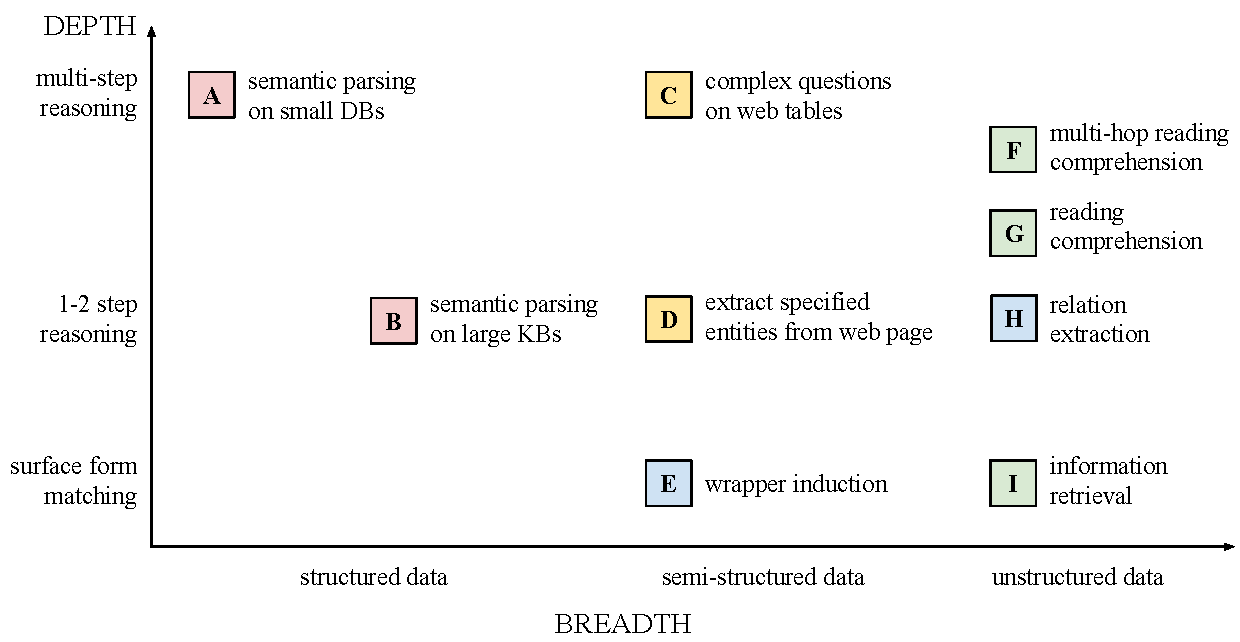
\includegraphics[width=\textwidth]{figures/intro/breadth-depth.pdf}
\caption
[Comparison of related work in terms of \Breadth and \Depth]
{Comparison of retrieval-based QA (green),
knowledge-based QA (red),
and information extraction systems (blue) on
the scope of the knowledge source (\Breadth)
and the question complexity (\Depth).
This dissertation starts
with exploring semi-structured data
(Point~D),
and then progresses to a task that addresses
both \Breadth and \Depth
simultaneously (Point~C).}
\label{fig:depth-breadth-plot}
\end{figure}

These two classes of QA systems
traditionally operate on the opposite ends
of the spectrum.
As illustrated in Figure~\ref{fig:depth-breadth-plot},
retrieval-based QA works on open-domain unstructured data
(high \Breadth)
but traditionally aims to answer questions
that do not require multi-step reasoning
(low \Depth).
In contrast,
the strength of knowledge-based QA is its ability to
perform multi-step reasoning to answer complex questions
(high \Depth),
but the knowledge sources are traditionally constrained
to structured data with predefined schemata,
such as databases or knowledge bases
(low \Breadth).
The goal of this dissertation
(and several other recent works)
is to build QA systems that can
operate in high-\Breadth high-\Depth settings.

Finally in Section~\ref{sec:rw-ie},
we discuss \emph{information extraction} (IE) systems.
An IE system transforms unstructured or semi-structured data
into the structured format that knowledge-based QA systems can process,
which allows them to answer questions that are both complex
and open-domain.
The goal of most IE systems in the literature is to populate
a central structured knowledge source with a predefined schema.
While this allows information from multiple sources to be aggregated
in a systematic manner,
%this pipeline paradigm
%(extract information to get structured data, then apply QA)
the predefined schema,
along with precision and recall issues,
%this paradigm
%has several downsides that
inherently limits the amount of knowledge accessible by
the downstream systems.
As an alternative, the work in this dissertation employs
\emph{on-the-fly information extraction}:
instead of populating a central fixed-schema database,
we only convert parts of the source data
that are relevant to the question
into a temporary structured knowledge source.
Without a predefined schema, we are able to capture
more information from the source data;
however, we lose some benefits of having a unified database
(e.g., we can no longer aggregate data from different sources,
and running extraction for every question can be costly).
% We now also need a better QA system
% that can handle arbitrary data schemata.

%%%%%%%%%%%%%%%%%%%%%%%%%%%%%%%%%%%%%%%%%%%%%%%%%%%%%
\section{Knowledge sources}
\label{sec:rw-knowledge-sources}

We now classify the types of knowledge sources used
in QA systems based on
(1) the amount of structure specified
in the knowledge sources and
(2) whether the data schema is predefined.
The \Breadth axis in
Figure~\ref{fig:depth-breadth-plot}
lays out the different types of knowledge sources
described below.


\subsection{Structured data}

A structured knowledge source
has a well-defined \emph{schema}, which dictates
the types of objects that can exist in the knowledge source,
as well as the types of relations among them.
Database is a canonical example of structured knowledge sources:
the database schema defines the value type in each field,
the fields in each record,
and the relationship between records across database tables.
Other examples of structured knowledge sources
include
%databases (often contain data in some specific domain),
graph-structured
knowledge bases \cite{freebase2013dump,suchanek2007yago,auer2007dbpedia}
%(large and open-domain,
%with the types of graph nodes and edges defined by designers)
and constrained interactive environments
(e.g., a simulated world
with blocks that can be moved around).
Most knowledge-based QA systems,
such as natural language interfaces to databases \cite{androutsopoulos95nlidb}
and semantic parsers
\cite{zelle96geoquery,berant2013freebase,chen11navigate}
operate on structured knowledge sources.

Using a structured knowledge source
provides several benefits.
A structured knowledge source can store
a large amount of statistical data,
and usually provides a convenient interface
(e.g., database query languages)
for performing computation on such statistics.
Furthermore, structured data is a systematic way to consolidate knowledge.
In contrast to unstructured text
which may describe the same object,
relation, or event using a wide variety of paraphrases,
the schema of structured data forces the representation of information
to be unified and canonicalized,
making it easier to process.

On the flip side,
structured data presents a trade off between
knowledge coverage and maintainability.
Closed-domain structured knowledge sources,
such as a database for a specific application,
only support questions that are asked within that domain.
On the other hand,
open-domain structured knowledge sources,
such as large knowledge bases,
support a wider range of questions but
are difficult to populate and maintain.

Finally,
the fixed schema in structured data is both a blessing and a curse.
It is easier to design or learn a mapping between
natural language phrases in the question
and objects in the knowledge source
when the schema is known in advance.
However, the fixed schema limits the types
of knowledge that can be included in the knowledge source.

\subsection{Unstructured data}
\label{sec:rw-unstructured-data}

Unstructured knowledge sources are knowledge sources that
do not contain a schema.
While some QA works operate on \emph{unstructured media}
 such as 
images or videos,
most retrieval-based QA systems 
operate on \emph{unstructured text},
which we will focus on for our comparison.

A large amount of open-domain world knowledge is encoded
as unstructured text due to the flexibility
and expressiveness of natural language.
Apart from describing objects and their properties,
%as commonly seen in structured knowledge sources,
unstructured text is also used to express more complex structures
such as events and processes,
or more vague concepts such as arguments and opinions.
Using unstructured data as the knowledge source
opens the door for a much wider range of questions.

As its downside, unstructured text is more difficult
to process than structured data.
Due to the flexibility of natural language,
a QA system must be ready to handle
different sentence structures and 
linguistic patterns people use to express the same concept.
Additionally, compared to structured data,
plain text is a more clunky way to express a long series
(e.g., list of all national parks in United States)
or statistical data
(e.g., the area of each national park).
This means unstructured data is less suitable for questions
that require computation;
for instance, the data needed for computing the average area
of national parks is less likely to be expressed in plain text
(except when the average is already computed and explicitly stated in text).

\subsection{Semi-structured data}
\label{sec:rw-semi-structured-data}

Semi-structured data contains some semantic structures,
but the schema of such structures is not predefined
\cite{abiteboul1997querying,mchugh1997lore}.
Examples of semi-structured data include markup documents
(e.g., schema-less XML files and HTML pages)
and sections with uniform patterns within a document
(e.g., tables, bullet lists, and template-generated product listings
on web pages).
While a spcific data source might use the same schema
for all of its documents,
that schema would not apply to the similar type of content
from a different data source.

Semi-structured data inherits the advantages and disadvantages
from both structured and unstructured data.
Similar to structured data,
semi-structured data usually contains computable data,
but since the schema is not predefined,
it can express a variety of open-domain knowledge
depending on the author of the data.
On the flip side, the lack of a predefined schema
increases the difficulty of mapping
phrases in the questions to objects in the knowledge source.

%%%%%%%%%%%%%%%%%%%%%%%%%%%%%%%%%%%%%%%%%%%%%%%%%%%%%
\section{Types of questions}
\label{sec:rw-questions}

We now discuss the types of questions targeted by previous work
in question answering.
The family of questions our work focuses on is \emph{fact-based}
questions,
which have objective and mostly unique answers
with respect to the knowledge source
(e.g., \nl{Where was Barack Obama born?}
or \nl{What is the average earning of the company in 1999?}).
% Some previous works refer to these questions as
% \emph{factoid} questions,
% though the term ``factoid'' also carries the connotation of
% trivia-like questions that do not require complex reasoning to answer.
%
Other than fact-based questions,
previous work has also considered questions
whose answers are long explanations or opinions
\cite{burke1997question,soricut2006automatic}.
Most systems for answering such open-ended questions
treat the task as a information retrieval task,
where the potential answer snippets are retrieved and then ranked.

\subsection{Complexity in fact-based questions}

Most retrieval-based and some knowledge-based QA systems
target fact-based questions that only require simple reasoning
(sometimes called ``factoid'' questions).
As an example, consider the question
\nl{Where was Barack Obama born?}
asked under different knowledge sources.
When the knowledge source is a corpus of text documents,
a retrieval-based QA system can fetch a snippet that is likely
to contain the answer
(e.g., \nl{Obama was born on August 4 \dots in \textbf{Honolulu, Hawaii}.} from
the Wikipedia article \emph{Barack Obama}),
and then extract the answer
\nl{Honolulu, Hawaii} directly from a sentence in that snippet.
On the other hand, if the knowledge source is a structured database,
a knowledge-based QA system can identify the relevant entity
(\emph{Barack Hussein Obama})
and relation
(\emph{place of birth})
to find the answer.
In either cases,
given a portion of the knowledge source relevant to the question,
the answer can be computed using few steps of reasoning.

As stated in Chapter~\ref{chp:intro},
we want to build QA systems
that can answer complex questions
(i.e.,
high on the \Depth axis in Figure~\ref{fig:depth-breadth-plot}).
% but this does not necessarily means the questions
% have to be long or unnatural.
We consider the following sources of complexity
that can arise in fact-based questions.

\paragraph{Multi-step reasoning.}
% Many questions cannot be answered just by a single step of reasoning.
Performing multiple steps of reasoning
has been the goal of many knowledge-based QA
and interactive systems.
As an example, consider an early conversational system SHRDLU
\cite{winograd1972language},
which takes natural language commands or questions,
manipulates blocks in a simulated
three-dimensional environment,
and then generates natural language responses.
SHRDLU was designed to understand complex commands such as
\nl{Find a block which is taller than the one you are holding
and put it into the box.}
and
\nl{Is at least one of them narrower than the one which
I told you to pick up?}
(where \emph{them} refers to the answer from the previous question).
Another example is an early semantic parsing system
by \citet{zelle96geoquery},
which aims to answer highly compositional questions
such as
\nl{What states border states that border states that border states that border Texas?}
using a database as the knowledge source.

One common criticism of targeting multi-step reasoning
is the argument that humans rarely ask questions with complex linguistic constructs.
Indeed, since most commercial retrieval and question answering systems
(e.g., search engines and early virtual assistants)
cannot understand complex questions well,
the users have learned to ask simple questions
or even use a fragmented list of words
for such products.
Nevertheless, with the introduction of speech-enabled devices,
users have started to use natural language more often,
which increases the frequency of questions
that require multiple steps of reasoning
(though not as many steps as the examples given above).
% \citex.

\paragraph{Sublexical compositionality.}
Multi-step reasoning does not necessarily come from
questions with high linguistic compositionality.
Rather, depending on the type of information available in
the knowledge source,
even a simple word or phrase and invoke multi-step reasoning.
An example of such \emph{sublexical compositionality}
\cite{wang2015overnight}
is the question
\nl{Who is Barack Obama's \textbf{aunt}?}.
The question only requires one step of reasoning
if the knowledge source explicitly mentions the \emph{aunt} relationship.
However, for a database where only a person's parents,
siblings, and gender can be queried,
multiple steps of reasoning will be needed to answer the question.
Several other examples include
\nl{weekend} (Saturday or Sunday),
\nl{same position as John}
(people with the same position as John, except John himself),
and \nl{win} (might require summing up the scores to be compared).

\paragraph{Diversity of operators.}
Another potential source of complexity in fact-based questions
comes from the types of reasoning needed to compute the answer.
For instance, a QA system dealing with statistics
should be able to perform comparison
(\nl{Which company has the highest revenue?}),
aggregation
(\nl{What is the average revenue of tech companies?}),
and computation
(\nl{How much more does Walmart make than Apple?})
on the numerical data in the knowledge source.

As we will discuss in Section~\ref{sec:rw-knowledge-based-qa},
many knowledge-based QA systems use \emph{logical operators}
to represent types of reasoning.
Within this framework, the system has to choose the correct
logical operators, their arguments, and the order they should be composed
to compute the answer.
This can be challenging as the number of possible combinations
of operators scales with the size of the knowledge source
and grows exponentially with the number of reasoning steps.

%%%%%%%%%%%%%%%%%%%%%%%%%%%%%%%%%%%%%%%%%%%%%%%%%%%%%
\section{Retrieval-based question answering}
\label{sec:rw-retrieval-based-qa}

We now discuss the first family of question answering systems,
retrieval-based QA,
which is often used to handle open-domain questions
on unstructured knowledge sources.
To answer a given fact-based question,
most retrieval-based QA systems
(1) retrieve snippets from the knowledge source
that are relevant to the question,
and then (2) use reading comprehension to extract the answer
from the retrieved snippets.

\paragraph{Snippet retrieval.}
Given the question,
the task of snippet retrieval is to fetch portions of the knowledge source
that are relevant to the question,
and then rank them based on relevancy.

For fetching the candidate snippets to be ranked,
the most basic method is to find documents
with large word overlap with the question.
Weighting schemes such as tf-idf is often used
to emphasize the matching of important content words
\cite{jones1972tfidf,robertson2009probabilistic}.
To increase recall,
previous work has also used query expansion and query rewriting
to generate similar queries for retrieving a larger number
of relevant snippets
\cite{carpineto2012expansion}.

Various factors can be considered when ranking the snippets.
For instance, given user ratings as training data,
previous work considered training a supervised model
to assign scores to the retrieved snippets
\cite{cao2006adapting,yue2007support}.
Other factors such as prominence or credibility of the sources
can also be taken into account
\cite{haveliwala2002topic,gyongyi2004combating}

\paragraph{Reading comprehension.}
Given a snippet for the question,
the next step is to extract the answer from the snippet.
Early work in reading comprehension analyzes the question type
and uses linguistics patterns to extract the answer
\cite{brill2002askmsr,pasca2003open}.
With the availability of larger datasets and neural models,
more recent works cast reading comprehension as
predicting a token span inside the given snippet
\cite{yang2015wikiqa,rajpurkar2016squad,seo2016bidaf}.
This generally involves embedding the snippet and the question,
computing interaction between the two,
and then outputting the start and end positions of the span.
For fact-based questions with few steps of reasoning,
such neural models have matched the human performance
on many benchmarks \cite{chen2016thorough,devlin2018BERT}.

\paragraph{Increasing question complexity.}
Traditionally,
the questions that retrieval-based QA applies on
are usually ``factoid'' questions
that do not involve multi-step reasoning
\cite{voorhees1999overview,brill2002askmsr,pasca2003open}.
However,
more recent work has started to move toward
questions that require more complex reasoning.
% Early question answering systems
% (Point~J in Figure~\ref{fig:depth-breadth-plot})
% focus on retrieving the documents
% related to the question
% and extracting the relevant passage.
% The task of extracting more fine-grained answers
% started off with answer span extraction
% (Point~H)
% usually involving locating the correct context in a paragraph
% or document
% Later reading comprehension tasks
% demand more complex reasoning
% (Point~G):
% determining if a question is answerable
% requires reasoning beyond surface form matching
% \cite{rajpurkar2018squadrun},
% and many datasets contain
% questions with multi-hop reasoning over multiple pieces of evidence
% \cite{yang2018hotpotqa,dua2019drop}.
For instance,
datasets such as SQuAD 2.0 \cite{rajpurkar2018squadrun}
and Natural Questions \cite{kwiatkowski2019natural}
require the system to reason whether the question can be answered
by the given snippet.
The DROP dataset \cite{dua2019drop}
contain questions that require various types of operations
such as cross-referencing, comparison, and calculation
to compute the answer.
And the HotpotQA dataset \cite{yang2018hotpotqa}
requires two-step reasoning
where a second snippet has to be retrieved
based on the information gained from the first snippet.

Nevertheless, the types of questions and their complexity
are still partially limited by the nature of the knowledge source.
As discussed in Section~\ref{sec:rw-unstructured-data},
questions that require aggregating the attributes
of many entities 
(e.g., \nl{What is the average revenue of \dots?}
or \nl{Who is the oldest \dots?}) are usually covered by structured
or semi-structured data rather than unstructured text.

\paragraph{Question answering on images.}
As a side note,
a similar trend of increased question complexity
has also been observed
in the related task of visual question answering.
After the success of object recognition
\cite{krizhevsky2012imagenet,szegedy2015googlenet,he2016resnet}
and image captioning
\cite{farhadi2010every,lin2014microsoft,fang2015captions,mao2015deep},
researchers turned to the task of answering questions about the images.
Most earlier works consider
either simpler questions on diverse images \cite{antol2015vqa}
or complex questions on synthetic images \cite{johnson2017clevr,suhr2017nlvr}.
However, recent work has moved toward considering
higher \Breadth and \Depth simultaneously:
understanding complex questions
in the context of open-domain images
\cite{suhr2018situated,hudson2019gqa}.

%%%%%%%%%%%%%%%%%%%%%%%%%%%%%%%%%%%%%%%%%%%%%%%%%%%%%
\section{Knowledge-based question answering}
\label{sec:rw-knowledge-based-qa}

Knowledge-based QA systems perform reasoning on the facts
in the knowledge source
to compute the answer.
Among different ways to perform reasoning,
we focus on the \emph{semantic parsing} approach,
which we use for our main task.
In semantic parsing,
the steps of computation are represented as a discrete representation
called a \emph{logical form},
and the task is thus to map the given question into a logical form
that represents a correct way to compute the answer.

\subsection{Executable semantic parsing}

Broadly speaking,
\emph{semantic parsing} is the task of mapping
natural language utterance to \emph{some}
meaning representation.
As different subfields of natural language processing
employ different schemes of meaning representations,
the term ``semantic parsing''
has become a heavily overloaded term.
The possible interpretations include
shallow intent-slot tagging in dialog systems
\cite{pieraccini1991stochastic,raymond2007generative,mesnil2014using},
identifying semantic frames \cite{gildea02semantic,hermann2014semantic},
and
generating full semantic representations
such as abstract meaning representation (AMR) \cite{banarescu2013amr,flanigan2014discriminative,wang2015transition,artzi2015broad}
among many others.

For the purpose of question answering,
we will focus on \emph{executable semantic parsing},
which is based on
model-theoretic formal semantics \cite{montague73ptq}.
In this framework,
the semantic representations are interpreted under
the knowledge source (traditionally called a ``model'').
The result of this interpretation is called \emph{denotation},
which denotes some part of the knowledge source.
For instance,
in a database of countries in the world,
the denotation of $\T{CapitalOf}(\T{France})$
is a single entity $\T{Paris}$,
while the denotation of $\T{CapitalOf}$
is the mapping between countries and their capital cities.

In practical terms,
executable semantic parsing
is the task of mapping the input utterance $x$
into a semantic representation $z$
(usually called \emph{logical forms})
that can be executed like a computer program
on the knowledge source $w$
to give some desired denotation $y = \deno{z}{w}$.
For instance, the utterance $x =$ \nl{Tell me what 2 + 2 is.}
can be mapped to $z = \T{add}(2, 2)$, which can be executed
to give the denotation $y = 4$.
The logical form is not required to capture
all semantic details of the utterance
as long as its denotation under the knowledge source is correct
(e.g., in the example above,
the \emph{Tell me} part is not represented
in the logical form).

Semantic parsing has been applied in many tasks
that require compositional reasoning.
Some examples include:
parsing questions into database queries for retrieving the answers
\cite{zelle96geoquery,zettlemoyer07relaxed,berant2013freebase,dong2016logical,zhong2017seq2sql},
parsing the user's queries into API calls
\cite{quirk2015language},
parsing commands for navigating an agent
\cite{chen11navigate,tellex2011understanding,artzi2013weakly,andreas2015alignment},
parsing commands for manipulating objects
\cite{guu2017bridging,fried2018unified},
and parsing specifications into code in a programming language
\cite{kushman2013regex,ling2016latent,yin2017syntactic,rabinovich2017abstract,iyer2018mapping}.

% We now give a brief comparison
% in terms of \Breadth
% and \Depth
% between our work
% and previous semantic parsing work.
In the following subsections,
we will focus on works in semantic parsing for question answering
that have motivated our task settings.
% The discussion of later works and other settings
% will be deferred
% to Chapter~\ref{chp:tables}.
% We will focus on semantic parsing for question answering,
% which is the closest to our main task of
% answering question on web tables,
% and defer the discussion of other settings to
% Section~\ref{sec:wtq-other-datasets}.

\subsection{Highly compositional semantic parsers}

Early semantic parsing systems focus on
understanding very complex utterances in a
predefined domain.
For example, the
SHRDLU system \cite{winograd1972language}
mentioned earlier
can understand very compositional commands
such as
\nl{Find a block which is taller than the one you are holding
and put it into the box.}, but with hand-crafted rules,
it is difficult to generalize to linguistic variations
or larger knowledge sources.
Another example is the work by \citet{zelle96geoquery},
which learns to parse questions about geography
into database queries.
Again, the system targets highly compositional questions,
% (with perhaps the most famous example being
% \nl{What states border states that border states that border states that border Texas?}),
but the database used
is small and fixed.

Following \citet{zelle96geoquery},
the main focus of semantic parsing work
in the next decade
was on incorporating
statistical models into the parser.
By training the parser to predict the annotated logical forms
in the training data
\cite{kate07krisper,zettlemoyer07relaxed,kwiatkowski11lex},
the parser becomes more robust to lexical variations.
However, the knowledge sources these work consider
are still limited to small, fixed, and closed-domain databases.
In fact, one capability these models are expected to learn
is the association between the finite number
of objects in the knowledge source and 
input natural language phrases.

\subsection{Learning from denotations}
Training a statistical model for semantic parsing
requires some form of supervision.
The most straightforward supervision is to annotate
each question $x$ with a logical form $z$,
and then train the model to prefer the annotated $z$
over other logical forms.
However,
while logical form is a very strong signal,
it often requires expertise and time to annotate,
making it difficult to scale up to larger datasets
or larger knowledge sources.

Instead, previous work has considered using
the denotation $y$ (e.g., the correct answer to the
question $x$) as the form of supervision
\cite{clarke10world,liang11dcs}.
The model is now trained to prefer any logical form $z$
that executes to the annotated denotation $y$.
Denotations are easier to annotate by non-experts,
making it cheaper to scale up to larger-scale data.
Moreover, denotations are not tied to any formalism
of semantic representations,
making the dataset easier to use in different training paradigms
with different semantic representations.
The tasks in this dissertation will use denotations as supervision.

\subsection{Scaling up to large knowledge bases}

To expand the scope of the knowledge source,
later semantic parsing works consider using
large knowledge bases as the source of information
\cite{cai2013large,berant2013freebase}.
These knowledge bases such as
Freebase \cite{freebase2013dump} contain
millions of entities and relations
across multiple domains.
In order to handle the increased \Breadth
of the knowledge source,
previous work employs various techniques such as
paraphrase models \cite{berant2014paraphrasing}
and distributional representations \cite{bordes2015simple}
to link natural language to the corresponding
objects in the knowledge base.
Unfortunately,
as the trend shifts toward handling \Breadth,
the questions these work consider are often
much less compositional.
For instance, the commonly studied
\Sc{WebQuestions} dataset \cite{berant2013freebase}
and the subsequent \Sc{SimpleQuestions} dataset
\cite{bordes2015simple}
of factoid questions on Freebase,
most questions can be answered by identifying the correct
entity (e.g., \emph{Barack Obama})
and relation (e.g., \emph{place of birth})
\cite{yao2014freebase}.

Another important point to note is that while knowledge bases
contain information from many domains,
the included information is inherently limited
by the rate in which the data gets populated,
and by the data schema set up by the knowledge base maintainer.
This makes knowledge bases not fully open-domain.
Research on knowledge base population \cite{ji2011knowledge,ellis2015tackbp,stanford2017kbp}
and attribute discovery \cite{cafarella2008webtables,yakout2012infogather}
tries to address these issues,
but it would be more preferable if a semantic parsing system
can process open-domain data from the source directly
instead of waiting for the knowledge base to be populated.

\subsection{Semantic parsing on open-domain tables}

Our work on complex question answering on web tables
aims to increase the scope of the domain
by using web tables as the knowledge source,
while at the same time bring back the compositionality
in the input questions.
Even though the table is much smaller than a knowledge base,
different questions are asked on different tables
with possibly unseen schemata,
making it more open-domain than a fixed knowledge base.
As for task complexity,
while the questions in our dataset are not as compositional
as the extreme examples from earlier works,
they still require non-trivial numbers of steps
and a diverse type of operations (e.g., aggregation,
comparison, calculation) to derive the answers.

After our work, there have been a few other tasks
and datasets related to question answering on open-domain tables.
Notable ones include the \Sc{WikiSQL} dataset
\cite{zhong2017seq2sql},
which focuses on identifying table columns and values
in the \T{SELECT} and \T{WHERE} clauses of SQL queries;
and the \Sc{Spider} dataset
\cite{yu2018syntaxsqlnet,yu2018spider},
which considers very complex SQL queries add incorporates
multiple tables with \T{JOIN} clauses.
We will compare our dataset with these related datasets
in Chapter~\ref{chp:tables}.

\subsection{Reasoning without discrete logical forms}
Discrete representation, such as logical forms,
is not the only way for computing the answer to a complex question.
With the recent development of using neural network
as a universal computation device
\cite{graves2014neural,weston2015memory,reed2016neural},
previous work has considered representing
the intermediate result of multi-step computation
as a continuous state vector
\cite{neelakantan2016neural,yin2016neural,mou2017coupling,iyyer2017search}.
Under this paradigm,
a neural model takes in the question and the knowledge source,
and then updates the state vector for several time steps.
The final state vector is then used to produce the final answer.
Chapter~\ref{chp:conclusion} describes the details of previous works
that utilize continuous representations to tackle the main dataset
of this dissertation.

One benefit of using continuous representations
is the ability to train the model in an end-to-end fashion.
% It avoids the problem of searching over the exponentially many
% combinations of discrete symbols as required by
% the semantic parsing approaches.
However, compared to the semantic parsing approaches
that use discrete logical forms,
the continuous representation is less interpretable,
making it difficult to diagnose mistakes.
Moreover, learning to perform complicated operations
(e.g., subtracting the start date from end date for each event)
requires a large amount of training data and
a model expressive enough
to encode the operations.

% In Chapter~\ref{chp:conclusion},
% we will return to discuss previous works that use
% neural reasoning to answer questions on semi-structured tables,
% and contrast them with our semantic parsing approach.

%%%%%%%%%%%%%%%%%%%%%%%%%%%%%%%%%%%%%%%%%%%%%%%%%%%%%
\section{Information extraction}
\label{sec:rw-ie}

The main goal of this dissertation is to create a system
for understanding complex questions (high \Depth)
that works directly on open-domain data (high \Breadth).
Instead of this challenging paradigm,
one alternative solution to creating a system in
a high-\Breadth high-\Depth regime is a pipeline approach:
apply an \emph{information extraction} (IE) system to
convert the source unstructured or semi-structured data into a
structured knowledge source (e.g., a database),
and then have a knowledge-based QA system
use the populated structured data to answer complex questions.
In this section,
we give an overview of previous work on information extraction,
and then explain the limitations of this pipeline approach.

\subsection{Information extraction on unstructured text}

As most databases and knowledge bases represent relations between objects,
one common information extraction task is \emph{relation extraction}:
extract binary relations between two entities mentioned
in the text
(e.g., from the snippet
\nl{Obama was born on August 4 \dots in Honolulu, Hawaii},
extract the relation \emph{place of birth}
between \emph{Barack Obama} and \emph{Honolulu, Hawaii}).
Early relation extraction works find snippets that express
the desired relations with explicit
linguistic patterns, which can be manually written or bootstrapped
\cite{hearst1992automatic,hearst1998automated,agichtein2000snowball}.
Later works learn classifiers to detect relations between entity mentions.
To train the classifiers, previous works consider using
texts annotated with relation as a direct supervision
\cite{zeng2014relation,miwa2016end}
or known relations between entities as a distant supervision
\cite{mintz2009distant,riedel2010modeling}.

When the exact relations to extract is not given,
\emph{open information extraction} can be used instead
\cite{banko2007open,fader11reverb,etzioni11openie,masaum2012open,mitchell2015nell}.
These systems take unstructured text and extract
binary relations between entities,
where the relation is derived from the text string
instead of a predefined list of relations.

Beyond binary relations between two entities,
previous work has also considered extracting more complex structures
such as events and temporal series of events
\cite{riedel2011robust,li2013joint,chen2015event}.

\subsection{Information extraction on semi-structured data}

The main line of works on information extraction from semi-structured data
is \emph{wrapper induction}
\cite{kushmerick1997wrapper,crescenzi2001roadrunner,dalvi2011automatic}.
We give a brief overview of wrapper induction
and defer the details to Chapter~\ref{chp:semi}
when we discuss our proposed task of entity list extraction.
A \emph{wrapper} is
any machinery (e.g., a pattern or a program)
that extracts the information specified by the user.
For instance, on a web page,
selectors such as regular expressions and 
XPaths have been used as patterns for extracting the desired information.
The process of inducing a wrapper is called wrapper induction,
which is usually done based on a few given examples 
of the extraction targets.
From the examples,
a wrapper generator generates candidate wrappers that correctly extract
the examples,
and then a ranker ranks the wrapper to find the one that is likely
to generalize to new source documents.

\subsection{Advantages and disadvantages of the pipeline approach}

We now examine the pipeline approach of
extracting information from open-domain data and then
applying knowledge-based QA on the populated database.
With the clear separation of the two pipeline steps,
it is easier to develop the information extractor and
semantic parser independently.
The resulting database is highly interpretable
and can be directly used outside the context of semantic parsing.
Moreover, information from multiple data sources
can be \emph{aggregated} to form a unified consensus of the data.
This increases the factual correctness when answering questions
(e.g., for \nl{Where was Barack Obama born?},
some documents give a wrong answer),
and increases the coverage when the answer is an open-ended list
(e.g., \nl{What are some important buildings in New York?}).

However, the pipeline approach also has several limitations.
First, information extraction
can produce errors that are propagated to the database
(``precision'' problem).
This can sometimes be mitigated by leveraging redundancy
and verifying the extracted facts across multiple sources.
% but for niche data with no redundant documents,
% such verification is impossible to do.

Second, data extraction is a lossy process
and could discard a large amount of information from the source documents
(``recall'' problem).
For example, information that has to be inferred from
multiple sentences are generally difficult to detect.
%\todo{give a concrete example}
This limitation can be quite severe even when extracting
information in non-specialized domains.
In knowledge base population challenges \cite{ji2011knowledge,ellis2015tackbp},
in which specified properties about the specified entities
should be extracted from text documents,
the recall of even the best system is usually much lower
than the human's performance.

Finally,
the types of extracted data
is limited by the schema of the database.
Handling questions outside the database schema
requires solutions such as knowledge inference
based on other existing information \cite{nickel2011three,riedel13universal,neelakantan2015compositional}
or rerunning the information extractor to extract the required information.

\subsection{On-the-fly information extraction}

Semi-structured data, such as web pages and web tables,
contains an arbitrary schema depending on the whim of its authors.
As such, in order to retain as much knowledge as possible
from a semi-structured knowledge source,
we should not force the extracted data to conform to a predefined schema.
Instead of populating a central database with a predefined schema,
an alternative approach we take is
\emph{on-the-fly information extraction}:
upon retrieving the relevant snippets from the knowledge source
(e.g., a web table),
we apply IE to create a temporary structured data
just for that snippet.
The schema of the produced structured data depends on
the source data,
which allows it to represent any types of relation present
in the source data.
However, this increased flexibility comes with a trade off:
since the schema is not predefined,
it is more difficult to map the phrase in the question
to the objects and relations in the produced structured data.

On-the-fly information extraction
has been explored by some previous QA systems.
For instance, the START system by \citet{katz2002omnibase}
first translates the user query into a logical form
(e.g., \nl{Who directed gone with the wind?}
is mapped to
\T{(get "imdb-movie" "Gone with the Wind (1939)" "DIRECTOR")}).
The execution of the logical form involves
fetching the web page specified by the logical form
(e.g., IMDB page for the movie \emph{Gone with the Wind}),
and then using a wrapper to extract the answer
(e.g., use an HTML wrapper to read off the director's name
from the information table).
Another example is the Octopus system \cite{cafarella2009data},
which facilitate data integration tasks.
From the given query (e.g., \nl{VLDB program committee}),
Octopus first retrieves and ranks a list of web tables matching the query.
The user can then use
data integration operators to aggregate
the retrieve information and construct a unified structured table.

%Assuming that the relevant portion of the knowledge source
%is already retrieved,
%we focus on
%(1) extracting structured data from the source data
%and (2) performing question answering on the resulting structure.


\chapter{Semi-Structured Data on Web Pages}
\label{chp:semi}
In this chapter,
we investigate the nature of \emph{semi-structured data}
on web pages,
as well as the techniques for handling them in
a question answering system.
As explained in Section~\ref{sec:rw-semi-structured-data},
a semi-structured knowledge source contains some form of structures,
but the schemata of such structures are not defined in advance.
For instance,
Figure~\ref{fig:openweb-running-ex} shows a web page
where hiking trails and their descriptions
are listed using a uniform structure.
However, there is no universal way
for presenting a list of hiking trails.
The webmaster gets to choose the pieces of information
to be presented in each entry
and how they should be laid out on the web page.
As such,
a different website might use a different data schema,
presenting different pieces of information in a different format.

\begin{figure}[t]
\centering
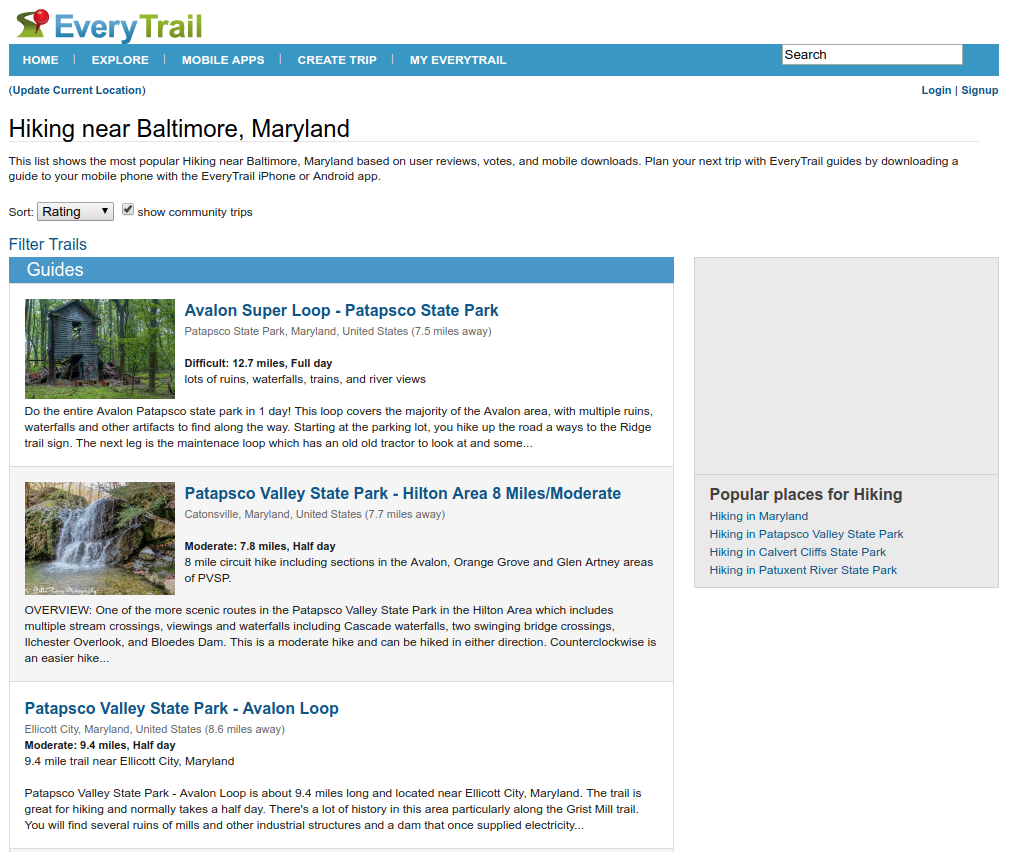
\includegraphics[scale=0.35]{figures/openweb/hiking-trails.png}
\caption[The list of hiking trails are presented in a semi-structured format on a web page.]{
The list of hiking trails are presented in a semi-structured format
on a web page. We consider the task of extracting
the specified list of entities
(e.g., \nl{hiking trails near Baltimore})
from the web page.}
\label{fig:openweb-running-ex}
\end{figure}

% Then in Section~\ref{sec:openweb},
% we consider the task of
% extracting a specified list of entities
% from the semi-structured data on the web page.
% (e.g., \nl{list of president names} $\to$
% \{``George Washington'', ``John Adams'', \dots\}).
% This task increases the focus on the structured part of the
% web page: the entity strings are to be extracted
% from the HTML elements with a coherent structure
% (e.g., cells from the same column of a table,
% or the header of each page section).

% Section~\ref{sec:openweb-compositional}
% gives several examples from
% our tasks that require compositional reasoning,
% which will serve as a motivation for the more complex task
% in later chapters.
% Finally, Section~\ref{sec:webpage-discussion}
% discusses related works on automated web interaction
% and information extraction from web documents.

To aid our investigation,
we consider the task of
extracting a specified list of entities
from the semi-structured data on the web page.
Concretely, given a natural language query
describing an entity category
and a relevant web page,
the task is to extract entities
that belong to the category from the page.
For example,
from the web page in Figure~\ref{fig:openweb-running-ex}
the question \nl{(What are) hiking trails near Baltimore}
should be mapped to the the list
\{\nl{Avalon Super Loop}, \nl{Patapsco Valley State Park}, \dots\}.
% Unlike information extraction from unstructured text
% \cite{hearst1992automatic,mintz2009distant,fader2014open},
% we can leverage the structured information on the web page:
% HTML elements containing entities of the same category
% usually have coherent structural properties.
% For instance, a web page showing a top-10 list
% usually have the ten entities as headers of the same level,
% and a web page with an information table might have
% the entities inside a single column of the table
% (excluding the column header).
We particularly focus on the semi-structured part of the
web page: the entity strings are expected to be extracted
from the HTML elements with a coherent structure
(e.g., cells from the same column of a table,
or the header of each page section).

We first formalize the task and give a few examples
from the \Sc{OpenWeb} dataset we collected for the task.
Afterward, we introduce \emph{extraction path},
an XPath-like latent selector
that selects HTML elements
that share the same structure.
The selected elements are then scores using
features that capture the homogeneity
of structural and linguistic information in the elements.
Finally, we present the experimental results of models
that were trained to generate good extraction paths.

\paragraph{Reference.}
The results described in this section have been published as
\citet{pasupat2014extraction}.

\section{The entity list extraction task}

\paragraph{Task.}
Given a web page $w$ (e.g., Figure~\ref{fig:openweb-running-ex})
and a natural language query $x$
(e.g., \nl{hiking trails near Baltimore}),
the task is to extracts a list $y$ of entities
that satisfy the query $x$
from the web page
(e.g., $y=$
\{\nl{Avalon Super Loop}, \nl{Patapsco Valley State Park}, \dots\}).

\paragraph{Dataset.}
We collected a new dataset, \Sc{OpenWeb},
with a diverse set of queries and web pages.
The data collection process is as follows:

\begin{enumerate}
\item
We used the method from \citet{berant2013freebase}
to generate a diverse set of search queries.
Specifically, we used the Google Suggest API,
which takes a partial query
(e.g., \nl{list of \blank movies})
and outputs complete queries
(e.g., \nl{list of horror movies}).

The queries were generated using breadth-first search
over the query space.
We started with the seed partial queries
\nl{list of $\bullet$\blank}
where $\bullet$ is one or two initial letters
(e.g., \nl{list of pr\blank}).
In each iteration, we called the Google Suggest API
to complete the queries,
and then applied the transformation rules in
Table~\ref{tab:openweb-suggest}
to generate more partial queries.
We ran the procedure until we obtained 100K queries.

\begin{table}[t]
\centering
\begin{tabular}{ll} \toprule
\textbf{Full query} & \textbf{New partial queries} \\
\midrule
list of $X$ IN $Y$
&list of $X$ \blank \\
where IN is a preposition
&list of \blank $X$ \\
(\emph{list of $[\text{hotels}]_X$ in $[\text{Guam}]_Y$})
&list of $X$ IN \blank \\
&list of \blank IN $Y$  \\
\midrule
list of $X$ CC $Y$
&list of $X$ \blank \\
where CC is a conjunction
&list of \blank $X$ \\
(\emph{list of $[\text{food}]_X$ and $[\text{drink}]_Y$})
&list of $Y$ \blank \\
&list of \blank $Y$ \\
\midrule
list of $X$ $w$
&list of $w$ \blank \\
(\emph{list of $[\text{good 2012}]_X$ $[\text{movies}]_w$})
&list of \blank $w$ \\
&list of $X$ \blank  \\
\bottomrule
\end{tabular}
\caption[
Rules for generating new partial queries
from complete queries.
]{Rules for generating new partial queries
from complete queries.
($X$ and $Y$ are sequences of words; $w$ is a single word.)}
\label{tab:openweb-suggest}
\end{table}

\item
For each query,
we downloaded the top 2--3 Google search results,
sanitized the web pages,
and randomly submitted 8000 web pages
along with their associated queries
to Amazon Mechanical Turk.
Each worker must either mark the web page
as irrelevant or identify the first, second,
and last entities (as strings) according to the query.
The dataset only contains examples where at least
two workers agreed on the three entities.
\end{enumerate}

The first, second, and last entities of the list
are used as a surrogate for the full list,
which is tedious to annotate.
We say that a list $y$ is \emph{consistent}
with the annotation if its first, second, and last entries
match the annotation.

\paragraph{Statistics.}
The \Sc{OpenWeb} dataset contains
2,773 examples from 2,269 distinct queries.
The queries span a variety of topics
from the more common ones
(e.g., movies, companies, characters)
to more obscure ones
(e.g., enzymes, proverbs, headgears).
The web pages are also diverse:
they come from 1,438 different web domains,
of which 83\% appears only once in the dataset.

Figure~\ref{fig:openweb-dataset} shows 
several queries and web pages from the dataset.
Besides the wide range of queries,
another main challenge of the dataset comes from
the diverse data representation formats such as 
tables, grids, lists, headings, and paragraphs.

\begin{figure}[t]
\centering
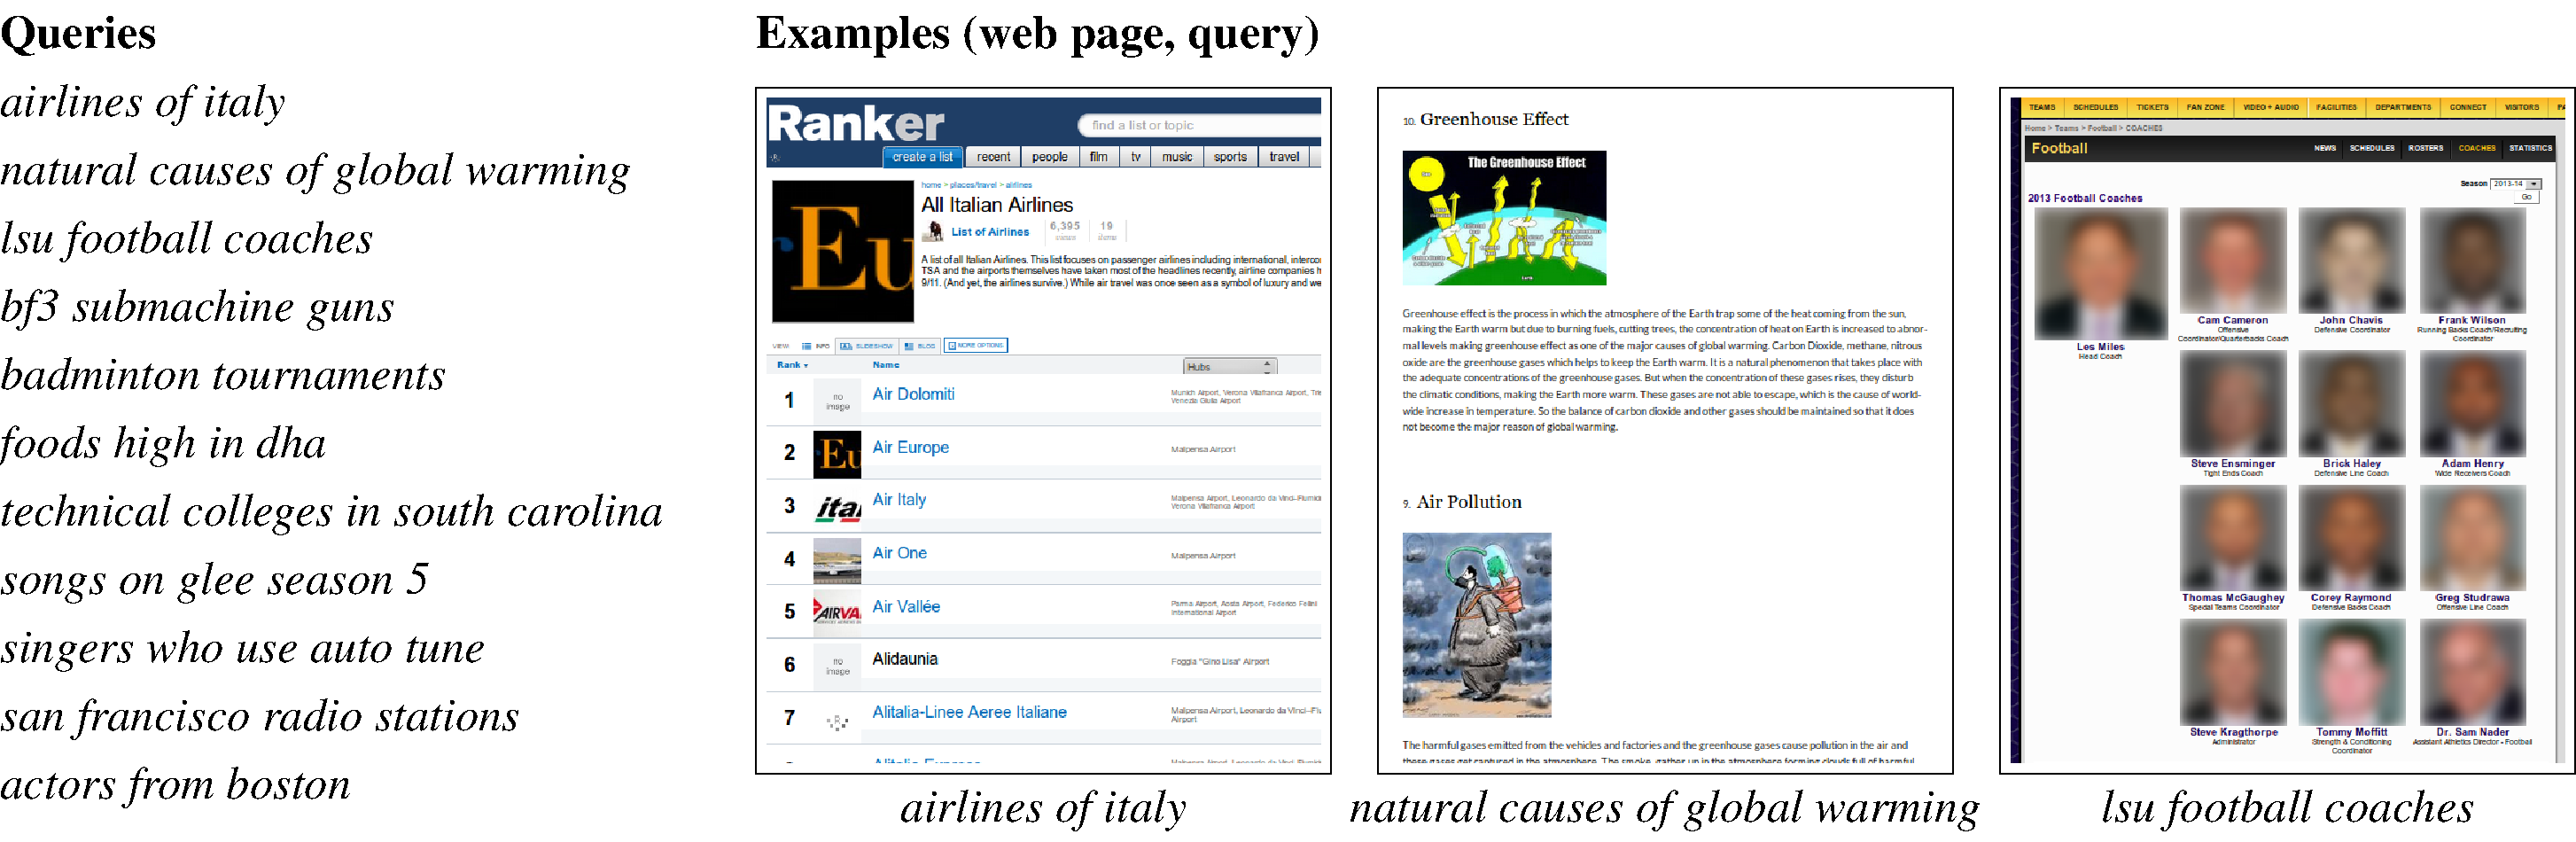
\includegraphics[width=\textwidth]{sfig/openweb.slides/extractionDataset.pdf}
\caption{Some examples illustrating the diversity of queries and web pages from the \Sc{OpenWeb} dataset.}
\label{fig:openweb-dataset}
\end{figure}


\section{Representation of the web page}\label{sec:openweb-representation}
The set of web pages across web domains form
a semi-structured knowledge source:
different web pages encode similar information
with different data schemata.
This schema mismatch sometimes manifests
even within the same web domain.
For example, while Wikipedia has guidelines on how
certain categories of articles should be formatted,
the data schemata still diverge drastically
between articles.

To handle arbitrary data schemata,
we propose to use a generic domain-independent structure
to represent web pages.
In particular,
we use the Document Object Model (DOM)
to represent the given web page $w$
as a tree of objects.
Unlike the full HTML DOM standard which includes multiple types of nodes
(e.g., text nodes and comment nodes),
we use a simplified representation
where all tree node are element nodes,
as shown in Figure~\ref{fig:openweb-extraction-path}.
For each DOM tree node,
we consider its HTML properties
(tag name and HTML attributes)
as well as its text content.
(The text content of non-leaf nodes
is the concatenation of all text content
within the subtree.)


\section{Extraction paths}\label{sec:extraction-paths}

We use latent \emph{extraction paths} $z$
to model the process of extracting entities
from the semi-structured web page $w$.
An extraction path is a simplified XML path (XPath) such as
\begin{equation}
z = \T{/html/body/table[2]/tr/td[1]}
\label{eqn:ex-xpath}
\end{equation}

Formally, an extraction path is a sequence of
\emph{path entries},
where each path entry is either a tag name (e.g., \T{tr})
or a tag name with an index (e.g., \T{td[1]}).
An extraction path $z$ can be executed on
the web page $w$ to get
$\deno{z}{w}$,
a list of matching HTML elements,
as follows:
\begin{itemize}
\item 
The base extraction path $z =$ \T{/html}
executes to a list containing
only the root \T{<html>} element of $w$.
\item
To execute $z\T{/}t$
(where $z$ is an extraction path and $t$ is a tag):
for each element $e \in \deno{z}{w}$,
select all children with tag $t$ of $e$.
Compile the selected elements into a list.
\item
To execute $z\T{/}t[i]$
(where $z$ is an extraction path, $t$ is a tag, and $i$ is an index):
for each element $e \in \deno{z}{w}$,
consider all children with tag $t$ of $e$,
and then select the $i$th one (1-indexed)
if there are at least $i$ such children.
Compile the selected elements into a list.
\end{itemize}

For example, as illustrated in
Figure~\ref{fig:openweb-extraction-path},
the extraction path
$z = \T{/html/body/table[2]/tr/td[1]}$
executes to the
first cell in each row of the second table on the page.
Note that all lists of elements are sorted
by the order they appear in the pre-order traversal
of the DOM tree.

\begin{figure}
\centering
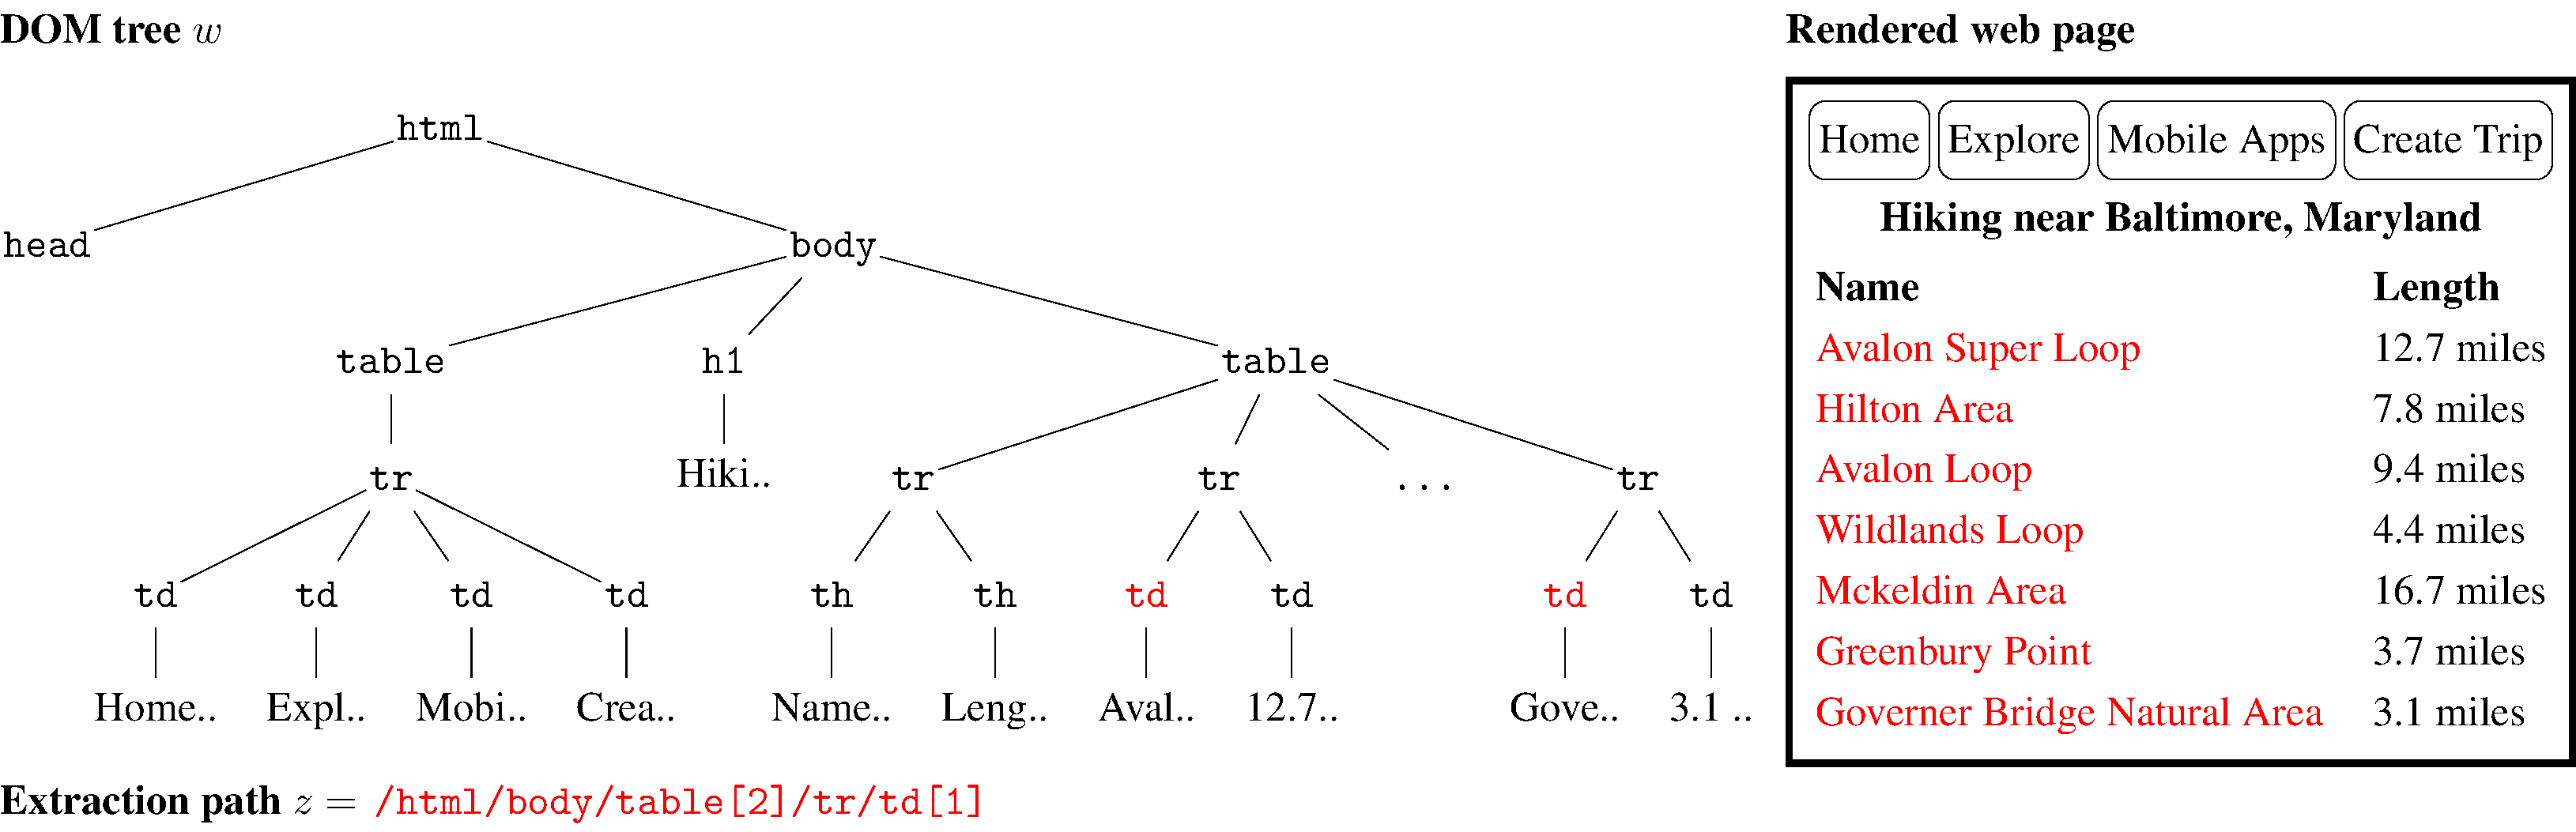
\includegraphics[width=\textwidth]{sfig/openweb.slides/extractionExample.pdf}
\caption[
Example of a DOM tree an extraction path.
]{A simplified example of a DOM tree of the web page $w$
and an extraction path $z$,
which selects a list of entity strings
$y = \deno{z}{w}$ from the web page (highlighted in {\color{red}red}).}
\label{fig:openweb-extraction-path}
\end{figure}

From the list $\deno{z}{w}$ of elements,
we can extract a list $y$ of entity strings
by compiling the text contents
of all elements in $\deno{z}{w}$
that are shorter than 140 characters.
This filtering is employed to control the search space.
This means an extraction path might yield an empty list of entities
(e.g., \T{/html/body/div[1]/p} gives no entities
if all the selected \T{<p>} elements contain
more than 140 characters).

\paragraph{Generating extraction paths.}
From a given web page $w$,
we can generate a set $\Mc{Z}(w)$ of candidate extraction paths
as follows.
For each element in the DOM tree,
we find an extraction path that selects only that element
(using only the indexed path entries),
and then generalizes the path by removing
any subset of indices of the last $k$ path entries.
For instance, when $k = 2$,
an extraction path ending in
\dots\T{/tr[5]/td[2]}
will be generalized to
\dots\T{/tr[5]/td[2]},
\dots\T{/tr/td[2]},
\dots\T{/tr[5]/td}, and
\dots\T{/tr/td}.
This generalization step allows us to select
multiple elements of the same structure
(e.g., table cells from the same column,
or list items from the same section).
We keep any generalized extraction path
where the extracted list of entities contain at least two entities.
Note that several extraction paths
might produce the same list of entities.

We use $k = 8$ in our experiments,
which gives at most $2^8$ generalized extraction paths
for each element.
Among the development examples of the \Sc{OpenWeb} dataset,
we generate on average approximately 8500 extraction paths,
which evaluate to approximately 1200 unique entity lists.

\section{Approach}
Given a query $x$ and a web page $w$,
we generate a set $\Mc{Z}(w)$
of candidate extraction paths $z$ as described
in Section~\ref{sec:extraction-paths}.
We then choose $z \in \Mc{Z}$ with the highest
model probability
$p_\theta(z \mid x, w)$
and extract the list of entities from $z$.

\paragraph{Model.}
From the query $x$ and the web page $w$,
we define a log-linear distribution over
the extraction paths in $\Mc{Z}(w)$ as
\begin{equation}
p_\theta(z \mid x, w) \propto \exp\crab{\theta^\top \phi(x,w,z)},
\end{equation}
where $\theta$ is the parameter vector
and $\phi(x,w,z)$ is the feature vector.

We train the model by maximizing the log-likelihood
of the extraction paths that
produce entity lists consistent with the annotation
(first, second, and last entities).
From training examples $(x\i, w\i, c\i)$,
where the indicator function $c\i(z)$ is 1 if
$z$ is consistent with the annotation and 0 otherwise,
we seek $\theta$ that maximizes
\begin{equation}
J(\theta) := 
\sum_{i} \log p_\theta(c\i = 1 \mid x\i, w\i) - \Omega(\theta)
\end{equation}
where
\begin{equation}
p_\theta(c = 1 \mid x, w)
= \sum_{z \in \Mc{Z}(w)} p_\theta(z \mid x, w)\,c(z)
\end{equation}
and $\Omega(z) = \frac{\lambda}{2}\norm{\theta}_2^2$
(with $\lambda = 0.01$)
is a regularization term.
We optimize $\theta$ with AdaGrad \cite{duchi10adagrad},
running for 5 epochs over the training data.

\section{Feature extraction}\label{sec:openweb-features}

The selected HTML elements from the web page $w$
contains both structured information
(e.g., their locations in the DOM tree)
and unstructured information
(e.g., their text contents).
As such,
we define the feature vector $\phi(x, w, z)$
as a concatenation of two types of features:
\emph{structural features} $\phi_\Mr{s}(w,z)$
which capture structured information of the HTML elements,
and \emph{denotation features} $\phi_\Mr{d}(x, y)$
which capture the linguistic information
of the extracted entity list $y$.

\begin{figure}
\centering
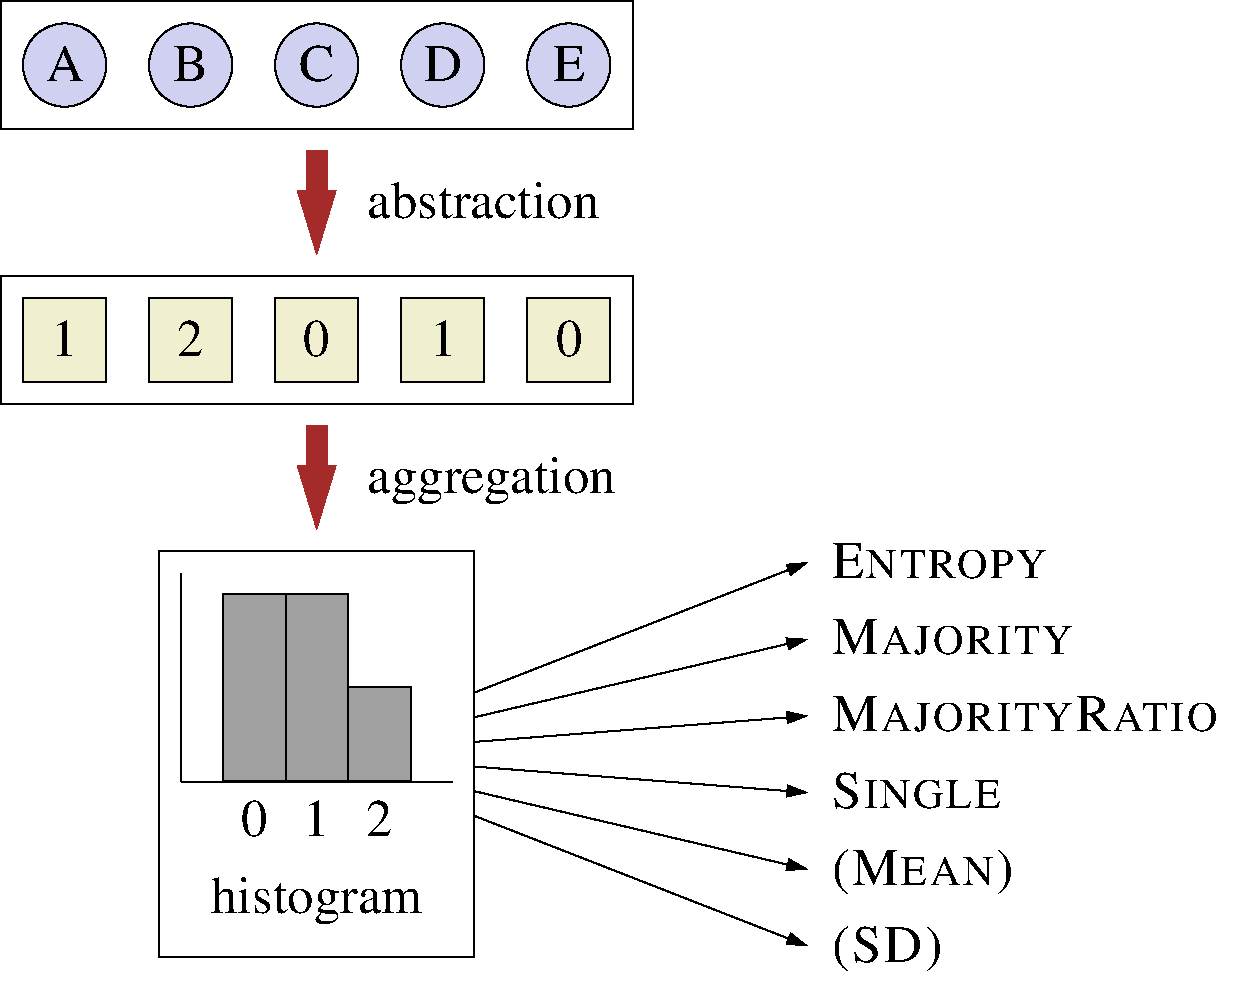
\includegraphics[width=0.5\textwidth]{sfig/openweb.slides/extractionFeatureRecipe.pdf}
\caption[
The recipe for defining features on a list of objects.
]{
The recipe for defining features on a list of objects:
(i) the \emph{abstraction} step converts list elements into abstract values;
(ii) the \emph{aggregation} step defines features using the histogram of the abstract values.}
\label{fig:openweb-recipe}
\end{figure}

\paragraph{Recipe for defining features on lists.}
Many of our features are defined on a list of objects
(e.g., a list of HTML elements or a list of entity strings).
When defining such features,
we want to incorporate the information about
individual list members,
as well as how the list looks like as a whole
(e.g., whether the members are diverse in some property).
As illustrated in Figure~\ref{fig:openweb-recipe},
we propose the following two-step recipe for generating
features from a list:

\begin{enumerate}
\item
\textbf{Abstraction.}
We map each list member to an abstract value
by extracting one of its properties.
For instance, we can map each each HTML element
to its number of children,
or map each entity string to its part-of-speech tag sequence.
\item
\textbf{Aggregation.}
We create a histogram of the abstract values,
and then define features based on the following statistics
of the histogram:
\begin{itemize}
\item \Sc{Entropy}: entropy normalized to the maximum value of 1.
The \Sc{Entropy} is 0 if all abstract values are identical,
and is 1 if all abstract values are distinct.
\item \Sc{Majority}: the most frequent abstract value.
\item \Sc{MajorityRatio}: percentage of abstract values
sharing the \Sc{Majority} value.
\item \Sc{Single}: whether all abstract values are identical.
\end{itemize}
For abstract values with finitely many possible values
(e.g., part-of-speech tags),
we also use the normalized count of each value as a feature.
And for numeric abstract values,
we also use the mean (\Sc{Mean}) and standard deviation (\Sc{SD}).
In our implementation,
real-valued features are converted to indicator features by binning.
\end{enumerate}

We use the recipe above to define structural features
and denotation features.
Figure~\ref{fig:openweb-features}
demonstrates some features we can extract from
the example in Figure~\ref{fig:openweb-extraction-path}.

\begin{figure}[t]
\centering
\begin{tabular}{cc}
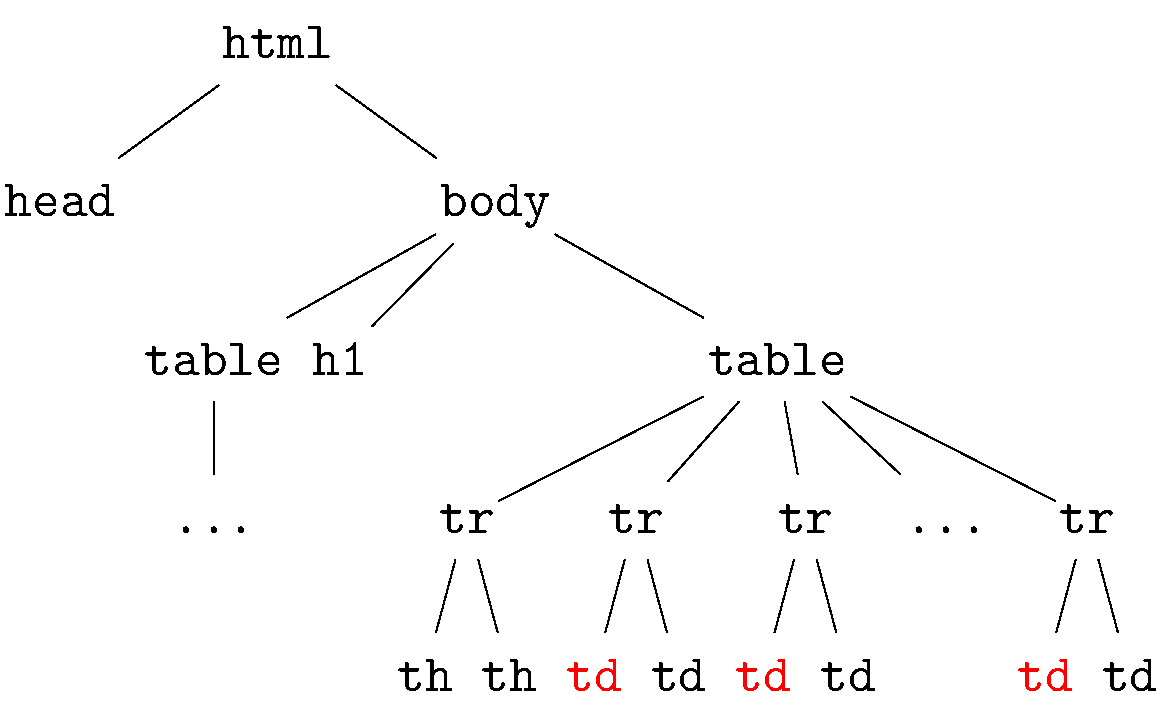
\includegraphics[scale=0.35]{sfig/openweb.slides/extractionFeatureStructural} &
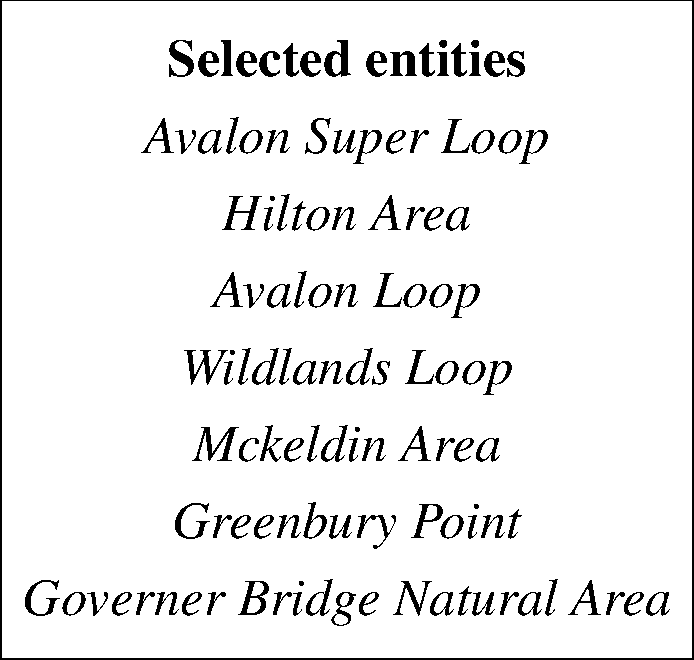
\includegraphics[scale=0.35]{sfig/openweb.slides/extractionFeatureDenotation} \\
\begin{tabular}[t]{ll} \toprule
\textbf{Structural feature} & \textbf{Value} \\ \midrule 
Features on selected nodes: \\
\quad\textsc{Tag-Majority} = \texttt{td} & 1\\
\quad\textsc{Index-Entropy} & 0.0 \\
Features on parent nodes: \\
\quad\textsc{ChildrenCount-Majority} = 2 & 1 \\
\quad\textsc{Parent-Single} & 1\\
\quad\textsc{Index-Entropy} & 1.0 \\
\quad\textsc{HeadHole} {\small (The first node is skipped)} & 1\\
Features on grandparent nodes: \\
\quad\textsc{PageCoverage} & 0.6 \\
\ldots & \ldots \\
\bottomrule
\end{tabular} &
\begin{tabular}[t]{ll} \toprule
\textbf{Denotation feature} & \textbf{Value} \\ \midrule 
\textsc{WordsCount-Mean} & 2.42 \\
\textsc{PhraseShape-Majority} = \texttt{Aa Aa} & 1 \\
\textsc{PhraseShape-MajorityRatio} & 0.71 \\
\textsc{WordShape-Majority} = \texttt{Aa} & 1 \\
\textsc{PhrasePOS-Majority} = NNP NN & 1\\
\textsc{LastWord-Entropy} & 0.74 \\ 
\textsc{WordPOS} = NN {\small (normalized count)} & 0.53 \\
\ldots & \ldots \\
\bottomrule
\end{tabular}
\end{tabular}

\caption[
A small subset of features from the example \emph{hiking trails near Baltimore}.
]{A small subset of features from the example \emph{hiking trails near Baltimore} in Figure~\ref{fig:openweb-extraction-path}.}
\label{fig:openweb-features}
\end{figure}

\paragraph{Structural features.}
Although different web pages represent data in different formats,
they still share some common hierarchical structures in the DOM tree.
We use structural features $\phi_\Mr{s}(w, z)$
to capture the structural information
from the extraction path $z$ and the selected elements $\deno{z}{w}$:

\begin{itemize}
\item \textbf{Features on the list of selected elements.}
We apply our recipe on the list of elements in $\deno{z}{w}$ using
the following abstract values of each element:
\begin{itemize}
\item The HTML \Sc{Tag} and attributes (\Sc{Id}, \Sc{Class}, \Sc{Href}, etc.)
\item \Sc{ChildrenCount}: the number of children of the element in the DOM tree.
\item \Sc{SiblingCount}: the number of siblings in the DOM tree.
\item \Sc{Index}: the position among its siblings.
\item \Sc{Parent}: the parent element
(e.g., the resulting \Sc{Parent-Single} feature indicates
that all elements share the same parent).
\end{itemize}

\item \textbf{Hole features.}
If the extraction path does not select all elements
in the same DOM tree level,
it is likely that the selection is incorrect.
For instance, an extraction path ending in \dots\T{/ul[1]/li/a}
selects links inside an unlabeled list.
However, if some list entries do not have links for some reason,
then the selected list will be incomplete.
In this case, it is preferred to use \dots\T{/ul[1]/li}
to select the list entries themselves instead.

To capture this intuition,
we define a \Sc{NoHole} feature
if all parents of the selected elements
has at least one of the selected elements as a child.
For the example above,
if some list entries \dots\T{/ul[1]/li} do not have links,
then the extraction path \dots\T{/ul[1]/li/a}
will not generate a \Sc{NoHole} feature.
To account for the common case of selecting table cells (\dots\T{/tr/td[$i$]}),
where the first row \T{<tr>} usually contains \T{<th>} instead of \T{<td>},
we define a \Sc{HeadHole} feature
if only the first parent is violating our criterion.

\item \textbf{Coverage feature.}
We define a real-valued feature \Sc{PageCoverage}
as the number of HTML elements that are descendents 
of the selected elements, divided by the total number of elements
on the web page.

\item \textbf{Features on ancestor elements.}
We also define the same feature set on the list of ancestors
of the selected elements.
In our experiments, we traverse up to 5 levels of ancestors
and define separate structural features on each level.

\end{itemize}

\paragraph{Denotation features.}
Structural features are not powerful enough
to distinguish entity lists with the same structure
(e.g., different columns of the table,
or different lists on the same web page).
To resolve this issue,
we define denotation features $\phi_\Mr{d}(x, y)$
on the entity list $y$ extracted from the selected elements:

\begin{itemize}
\item \textbf{Linguistic features.}
We observe that the correct entities often share 
some linguistic features.
For example, people and place names usually contain
2--3 word tokens with part-of-speech tag NNP (proper noun).
In contrast, incorrect lists of elements
(e.g., various \T{<div>} elements across the page)
tend to have texts of diverse lengths and linguistic tags.
With this reasoning, we apply our recipe on the list
of entity strings using the following abstract values
of each string:
\begin{itemize}
\item \Sc{WordCount}: number of tokens.
\item \Sc{PhraseShape}: abstract shape of the string
(e.g., \nl{Stanford University} becomes ``\T{Aa Aa}'').
\item \Sc{WordShape}: abstract shape of each word.
The features are defined on the list of words instead of the
list of entity strings.
\item \Sc{FirstWord} and \Sc{LastWord}
\item \Sc{PhrasePOS}: the part-of-speech sequence
of the whole string.
\item \Sc{WordPOS}: part-of-speech of each word.
Like \Sc{WordShape},
the features are defined on the list of words instead.
\end{itemize}

\item \textbf{Query-denotation features.}
Different query types denote entities
with different linguistic properties.
For instance, queries \nl{mayors of Chicago}
and \nl{universities in Chicago}
will produce entities of different lengths,
path-of-speech sequences, and word distributions.
This suggests incorporating features that depend
on the query $x$.

To this end, we define features of the form
$(f(y), g(x))$, where $f(y)$ is a linguistic feature
as described above, and $g(x)$ is the category of the query $x$.
For our experiments, we manually classify
the queries into 7 categories:
person, media title, location/organization,
abstract entity, word/phrase, object name, and miscellaneous.
In an actual system, the queries
should be classified automatically instead,
but we leave this as future work.
\end{itemize}

As the query-denotation features require
additional manual annotation,
we exclude them from the main experiments.
Instead,
we will investigate the effect of query-denotation features
in our model analysis (Section~\ref{sec:openweb-analysis}).

\section{Experiments}

We evaluate our model on the \Sc{OpenWeb} dataset.
The main evaluation metric is \emph{accuracy}:
the fraction of examples where
the model predicts an entity list consistent with the annotation.
We also report \emph{accuracy at 5},
the fraction of examples where one of the
five highest-scoring extraction path
yields a consistent entity list.
Finally, we report the \emph{oracle} score,
the fraction of examples where the model can
find at least one consistent entity list
among all extraction paths.

To measure how the consistency-based accuracy
tracks the actual correctness,
we sampled 100 web pages which have at least
one valid extraction path and manually annotate
them with the full entity lists.
We found that in 85\% of the examples,
the longest consistent list $y$ is the correct list,
and many lists in the remaining 15\%
miss the correct list by only a few entities.

\newcommand\sufpat[5]{\{\T{#1}, \T{#2}, \T{#3}, \T{#4}, \T{#5}\}}

\begin{table}[t]
\centering
\begin{tabular}{lr} \toprule
\textbf{Path suffix pattern} & \textbf{Count} \\ \midrule
\sufpat{a}{table}{tbody}{td[*]}{tr} & 1792 \\
\sufpat{a}{tbody}{td[*]}{text}{tr} & 1591 \\
\sufpat{a}{table[*]}{tbody}{td[*]}{tr} & 1325 \\
\sufpat{div}{table}{tbody}{td[*]}{tr} & 1259 \\
\sufpat{b}{div}{div}{div}{div[*]} & 1156 \\
\sufpat{div[*]}{table}{tbody}{td[*]}{tr} & 1059 \\
\sufpat{div}{table[*]}{tbody}{td[*]}{tr} & 844 \\
\sufpat{table}{tbody}{td[*]}{text}{tr} & 828 \\
\sufpat{div[*]}{table[*]}{tbody}{td[*]}{tr} & 793 \\
\sufpat{a}{table}{tbody}{td}{tr} & 743 \\ \bottomrule
\end{tabular}
\caption[
Top 10 path suffix patterns found by the baseline.
]{Top 10 path suffix patterns
found by the baseline.
We blank out the index numbers
and disregard the order of path entries,
making them a multiset instead of a sequence.
}\label{tab:openweb-baseline}
\end{table}

\paragraph{Baseline.}
As a baseline,
we list all 5-entry
suffixes of the correct extraction paths
in the training data,
and then sort the suffixes by frequency.
Table~\ref{tab:openweb-baseline}
shows the most frequent suffixes.
To increase generalization,
we blank out the index numbers
and discard the order of path entries.
At test time,
we choose an extraction path with the most
frequent suffix pattern.
The baseline should work reasonably well
if the web pages are relatively homogeneous.

\paragraph{Main results.}
We split the dataset into 70\% training and 30\% test data.
In addition to testing on test data,
we also report the results on 10 random 80-20 splits
of the training data.

\begin{table}[t]
\centering
\begin{tabular}{lcccc} \toprule
& \multicolumn{2}{c}{\bf 10 random splits} & \multicolumn{2}{c}{\bf Test data} \\
& \textbf{Acc} & \textbf{Acc@5} & \textbf{Acc} & \textbf{Acc@5} \\ \midrule
\textbf{Baseline} & 10.8 $\pm$ 1.3 & 25.6 $\pm$ 2.0 & 10.3 & 20.9 \\
\textbf{Our approach} & 41.1 $\pm$ 3.4 & 58.4 $\pm$ 2.7 & 40.5 & 55.8 \\
\textbf{Oracle} & 68.7 $\pm$ 2.4 & 68.7 $\pm$ 2.4 & 66.6 & 66.6 \\ \bottomrule
\end{tabular}
\caption[
Main results on the \Sc{OpenWeb} dataset.
]{Main results on the \Sc{OpenWeb} dataset
using the default set of features.
(Acc = accuracy, Acc@5 = accuracy at 5)}
\label{tab:openweb-main-results}
\end{table}

As reported in
Table~\ref{tab:openweb-main-results},
our approach gets a test accuracy of 40.5\%.
The oracle accuracy of 66.6\% reveals that there are
two categories of errors:
(i) \emph{coverage errors} (33.4\%),
which are when the system cannot find any
consistent entity list,
and (ii) \emph{ranking errors} (26.1\%),
which are when a consistent list of entities
exists but does not have the highest probability.

\begin{table}[p]\centering
\begin{tabular}{rp{5.5cm}p{6.5cm}r} \toprule
& \textbf{Reason} & \textbf{Example} & \textbf{Count} \\ \midrule
C1
& Answers and non-answer elements are selected by the same extraction path. 
& Select entries in the \nl{See Also} section
in addition to the content because they are all \texttt{<li>}.
& 48 \\ \midrule
C2
& HTML tag usage is inconsistent.
& The page uses both \texttt{<b>} and \texttt{<strong>} for headers
interchangeably.
& 16 \\ \midrule
C3
& The query applies to only some sections of the matching entities.
& Need to select only companies in China from the table of all Asian companies.
& 20 \\ \midrule
C4
& Answers are embedded in running text.
& Answers are in a comma-separated list.
& 13 \\ \midrule
C5
& Text normalization issues.
& Selected \nl{Silent Night Lyrics} instead of \nl{Silent Night}.
& 19 \\ \midrule
C6
& Other issues.
& Incorrect annotation / Entities are permuted when the web page is rendered
& 18 \\ \midrule
& \textbf{Total} & & 134 \\ \bottomrule
\end{tabular}

\caption{Breakdown of coverage errors from the development data.}\label{tab:webrep-coverage-errors}
\end{table}

\begin{table}[p]\centering
\begin{tabular}{rp{5.5cm}p{6.5cm}r} \toprule
& \textbf{Reason} & \textbf{Example} & \textbf{Count} \\ \midrule
R1
& Select non-content strings.
& Select navigation links, headers, footers, or sidebars.
& 25 \\ \midrule
R2
& Select entities from a wrong field.
& Select book authors instead of book names.
& 22 \\ \midrule
R3
& Select entities from wrong section(s).
& For the query \nl{schools in Texas},
select all schools on the page, or select the schools in Alabama instead.
& 19 \\ \midrule
R4
& Also select headers or footers.
& Select the table header in addition to the answers.
& 7 \\ \midrule
R5
& Select only entities with a particular formatting.
& From a list of answers, select only entities that are links (\T{<a>}).
& 4 \\ \midrule
R6
& Select headings instead of the contents or vice versa.
& Select the categories of rums in \T{<h2>} instead of the rum names in the tables.
& 2 \\ \midrule
R7
& Other issues.
& Incorrect annotation / Multiple sets of answers appear on the same page / etc.
& 9 \\ \midrule
& \textbf{Total} & & 88 \\ \bottomrule
\end{tabular}
\caption{Breakdown of ranking errors from the development data.}\label{tab:webrep-ranking-errors}
\end{table}

\section{Analysis}\label{sec:openweb-analysis}

Tables~\ref{tab:webrep-coverage-errors}~and~\ref{tab:webrep-ranking-errors}
show the breakdown of the coverage and ranking errors
on one of the development splits.

\paragraph{Analysis of coverage errors.}
From Table~\ref{tab:webrep-coverage-errors},
about 36\% of coverage errors happen when
the extraction path for the correct entities also 
captures irrelevant parts of the web page (Reason~C1).
For example, many Wikipedia articles contain
the \emph{See Also} section that lists
related articles in an unordered list
(\dots\T{/ul/li/a}).
This is problematic when the entities to be selected
are also represented in the same way.

Another main source of errors is the inconsistency
in HTML tag usage (Reason~C2).
For instance, some web pages use \T{<b>}
and \T{<strong>} interchangeably
for bold texts,
or switch between \T{<b><a>}\dots\T{</a></b>}
and \T{<a><b>}\dots\T{</b></a>} across entities.
Normalizing the web page,
using alternative web page representations,
or using a more expressive representation
than extraction paths could help reduce this type of errors.

\paragraph{Analysis of ranking errors.}
From Table~\ref{tab:webrep-ranking-errors},
a large number of errors are attributed to
selecting non-content elements such as
navigation links or content headings (Reason~R1).
It turns out that structural and linguistic
statistics of these elements can sometimes
be more coherent than those of the correct entities.
Since our features try to capture the
homogeneity of the selected elements,
the model can end up selecting these irrelevant elements.
A possible solution is to
detect the saliency of the element
and favor the elements that are in the content part
of the page.

\begin{table}[t]\centering
\begin{tabular}{lcc} \toprule
\textbf{Setting} & \textbf{Acc} & \textbf{Acc@5} \\ \midrule
All features & 41.1 $\pm$ 3.4 & 58.4 $\pm$ 2.7 \\
Oracle & 68.7 $\pm$ 2.4 & 68.7 $\pm$ 2.4 \\
\midrule
Structural features only & 36.2 $\pm$ 1.9 & 54.5 $\pm$ 2.5 \\
Denotation features only & 19.8 $\pm$ 2.5 & 41.7 $\pm$ 2.7 \\
\midrule
Query-denotation features only & 25.0 $\pm$ 2.3 & 48.0 $\pm$ 2.7 \\
Structural + query-denotation & 41.7 $\pm$ 2.5 & 58.1 $\pm$ 2.4 \\  \midrule
Concatenate a random web page + \\ \quad structural + denotation & 19.3 $\pm$ 2.6 & 41.2 $\pm$ 2.3 \\
Concatenate a random web page + \\ \quad structural + query-denotation & 29.2 $\pm$ 1.7 & 49.2 $\pm$ 2.2 \\
\bottomrule
\end{tabular}
\caption[
System accuracy with different feature and input settings on the development data.
]{System accuracy with different feature and input settings on the development data.
(Acc = accuracy, Acc@5 = accuracy at 5)}\label{tab:openweb-ablation}
\end{table}

\paragraph{Feature ablation.}
Table~\ref{tab:openweb-ablation}
shows the ablation results
on 10 development splits.
We observe while the structural features
are responsible for most of the accuracy,
denotation features is also helpful.
By examining the actual predictions,
we found that if there are multiple
parallel lists on the web page
(e.g., different columns of a tables),
denotation features help the system
select the correct list.
In contrast, structural features
act as a prior that
prevents the system from selecting
random entities outside the main part
of the web page.

\paragraph{Query-denotation features.}
The model so far does not include query-denotation features,
meaning that the input query $x$ is ignored entirely.
Despite this, since the web page
was obtained from a search engine,
the most prominent entities on the web pages
are likely to satisfy the query already,
and thus we were able to get some reasonable accuracy.

Table~\ref{tab:openweb-ablation}
shows that using only query-denotation features
(no structural features)
increases the accuracy over using 
normal denotation features
by 5.2\%.
When combined with structural features,
the query-denotation features help the model
select entities that are more appropriate for the query,
as shown in Table~\ref{tab:openweb-deno-example}.
However, it does not increase the
overall accuracy.
This is perhaps because the web page is already
related to the query as argued earlier.

\begin{table}[t]
\centering
\begin{tabular}{lll} \toprule
\textbf{Query} & \textbf{Default features} & \textbf{+ query-denotation} \\
\midrule
euclid’s elements book titles
& \nl{Prematter} & \nl{Book I. The fundamentals \dots} \\
(category = \emph{media title})
& \nl{Book 1} & \nl{Book II. Geometric algebra.} \\
& \nl{Book 2} & \nl{Book III. Theory of circles.} \\
& \dots & \dots \\ \midrule
soft drugs
& \nl{Hard drugs} & \nl{methamphetamine} \\
(category = \emph{object name})
& \nl{Soft drugs} & \nl{psilocybin} \\
& \nl{Some drugs cannot be classi\dots} & \nl{caffeine} \\
& \dots & \dots \\ \midrule
professional athletes
& ``\emph{Pistons-Knicks Game Becomes}
& \nl{Mike Richter} \\
with concussions
& \emph{\quad Site of Incredible Dance Battle}''
& \nl{Stu Grimson} \\
(category = \emph{person})
& \nl{Toronto Mayor Rob Ford \dots} & \nl{Geoff Courtnall} \\
& \dots & \dots \\ \bottomrule
\end{tabular}
\caption{The predictions after changing denotation features
into query-denotation features.}
\label{tab:openweb-deno-example}
\end{table}

To test query-denotation features
in scenarios where the most prominent elements
might not give correct entities,
we conduct experiments on a modified dataset
where in each example,
the original web page and an unrelated web page
are concatenated (in a random order).
We find that query-denotation features
(with structural features) significantly
improve the accuracy over using the normal
denotation features from 19.3\% to 29.2\%.


\section{Related work and discussion}
\label{sec:webpage-discussion}

\paragraph{Web page understanding.}
To understand the overall structure of web pages,
work on web page segmentation aims to segment the page
into semantically meaningful blocks
\cite{bing2014web,kreuzer2015quantitative},
identify salient parts of the web page
\cite{gamon2013identifying,shen2014webpage},
align the structures with the same semantics between web pages
\cite{kumar2011bricolage},
or detect the semantics of web page regions
\cite{spengler2010document,kumar2013webzeitgeist}.

\paragraph{Extracting information from web pages.}
Our presented approach is closely related to the work on
wrapper induction \cite{kushmerick1997wrapper}.
A wrapper is a function that takes the web page as input
and return the extracted information.
% For instance, our extraction path can be viewed as a wrapper.
Previous work on wrapper induction
mostly focuses on a small set of web domains,
and assume that the web pages follow a fixed template
\cite{muslea2001hierarchical,crescenzi2001roadrunner,cohen2002flexible,arasu2003extracting,dalvi2011automatic}.
Later work tries to generalize across web pages,
but relies on restricted data format \cite{wong2009scalable}
or prior knowledge of the web page structure
for the desired data to extract \cite{zhang2013automatic}.

Given a web page generated from a template
(e.g., a product listing page on an online shop),
previous work has also considered using
the regularity of web page elements
to extract structured information.
For instance, \citet{grigalis2014unsupervised}
extracts data records by looking at contiguous elements
that are visually similar,
and \citet{omari2016lossless}
factors the raw data from the web template.

Our setting differs from previous work on wrapper induction
in two major ways.
First, most previous works on wrapper induction
operate on a fixed website.
The induced wrapper only match the data schema of that website,
and is not likely to work on a different websites
or even a different version of the same website.
Similar to some previous work that generalize across pages
mentioned above
\cite{wong2009scalable,zhang2013automatic},
our approach does not make an assumption about the schema of the web page.
Second, in most wrapper induction systems,
the user specifies a few examples of entities to be extracted,
and the system tries to find wrappers that can extract
such entities.
Our setting has natural language as the specification
of what entities to extract,
which requires less effort from the user.
Note that 
while the query-dependent features has minor impact
on the overall extraction accuracy,
the features do help in scenarios where the most
prominent HTML elements on the page do not produce
the specified entities.

\paragraph{Collating information from web pages.}
Instead of extracting only the specified type of information,
one might want to mine and process all possible information
from a collection of web pages.
This can reveal corpus-level statistics that cannot be captured
by processing individual web pages.
For instance, WebTables \cite{cafarella2008webtables}
compiles a large corpus of web tables,
resulting in a corpus that can be used for many downstream tasks
such as deriving the correlation between data schemata (column headers).
Other works consider methods for processing
the mined data,
such as recovering the missing column headers \cite{venetis2011recovering}
or converting raw data to canonical formats
\cite{sarawagi2014open,embley2016converting}.

One way to view these families of information extraction methods
is to compare them with relation extraction from unstructured text (Section~\ref{sec:rw-ie}).
Wrapper induction and other query-based extraction methods
is parallel to relation extraction with
a predefined set of relations \cite{hearst1992automatic,mintz2009distant,miwa2016end}.
In contrast, WebTables and other works that collate information
from the structured parts of web pages
is parallel to open information extraction
\cite{banko2007open,fader11reverb,etzioni11openie,masaum2012open}.

\paragraph{Interacting with web pages.}
Previous work has considered a variety of interfaces
for humans to interact with web pages.
Some examples include
keystrokes \cite{spalteholz2008keysurf},
speech \cite{ashok2014wizard},
haptics \cite{yu2005haptics},
and eye gaze \cite{kumar2007eyepoint}.

In contrast to the methods above,
automated web scripts can be used for web page interaction
with minimal human intervention.
Most script frameworks refer to elements with logical selectors
such as CSS matchers and XPaths.
Due to the brittle nature of these selectors,
the script can break when the web page changes its layout,
or when the attributes of HTML elements are automatically generated
(either due to the web framework used or for obfuscation purposes)
\cite{hammoudi2016why}.

Previous work has proposed alternative methods
for referencing web elements in automated web scripts.
A few examples include Sikuli \cite{yeh2009sikuli},
which uses images of the elements,
and TagUI \cite{soh2017tagui},
which uses natural language.
These tools were designed for productivity,
but also have robustness as a side benefit.
For instance, even when an element changes its attributes
or location, a visual-based selector
will still be able to select it.

Instead of manually authoring the scripts,
previous work has also considered learning an agent
to perform actions on web page based on the given goal.
The agent can be learned
from demonstrations \cite{allen2007plow},
reinforcement learning
\cite{branavan08annotation,branavan09reinforcement}
or both \cite{shi2017wob,liu2018workflow}.

\paragraph{The need for compositionality.}

While doing error analysis,
we observe multiple examples that require
compositional understanding of the input query $x$
to obtain the correct answers.
A few of such examples are elaborated below:

%%%%%%%%%%

\begin{figure}[tp]
\centering
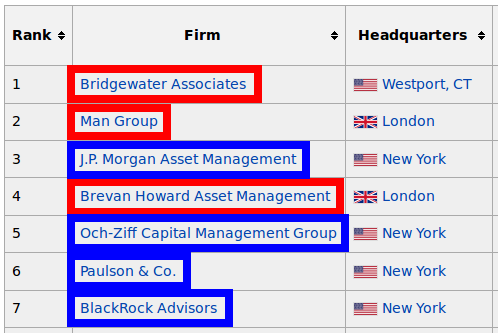
\includegraphics[scale=0.45]{figures/openweb/incorrect2-hedgefund.png}
\caption[
The query \nl{list of hedge funds in New York}
requires compositional understanding.
]{The query \nl{list of hedge funds in New York}
requires filtering the list of entities
by the value in the Headquarters column.}
\label{fig:openweb-hedgefund}
\end{figure}

\begin{figure}[tp]
\centering
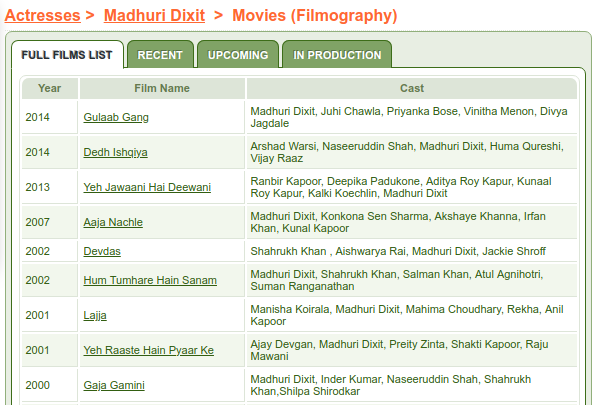
\includegraphics[scale=0.45]{figures/openweb/openweb-indian.png}
\caption[
The query \nl{list of Salman Khan and Madhuri Dixit movies}
requires compositional understanding.
]{The query \nl{list of Salman Khan and Madhuri Dixit movies}
requires filtering the list of entities
by the value in the Cast column.}
\label{fig:openweb-indian}
\end{figure}

\begin{figure}[tp]
\centering
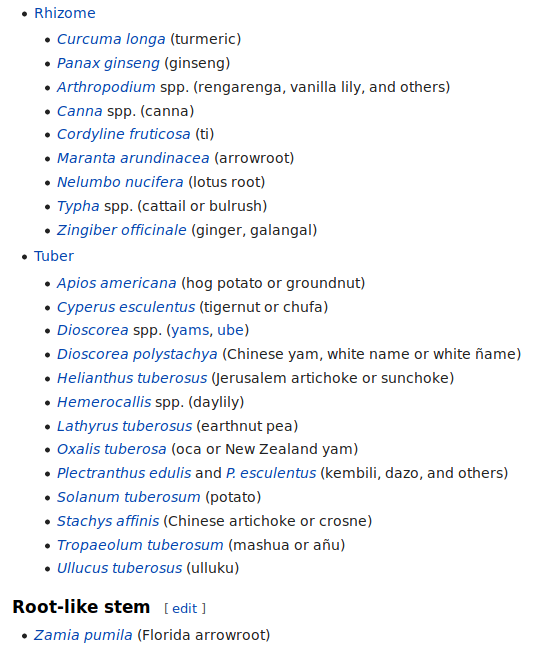
\includegraphics[scale=0.45]{figures/openweb/openweb-tubers.png}
\caption[
The query \nl{list of plants that are tubers}
requires compositional understanding.
]{The query \nl{list of plants that are tubers}
requires locating the correct portion of the list
based on the list indentation.}
\label{fig:openweb-tubers}
\end{figure}

%%%%%%%%%%

\begin{itemize}
\item In Figure~\ref{fig:openweb-hedgefund},
the query \nl{list of hedge funds in New York}
requires filtering the list of entities from
the Firm column by the values in the Headquarters column.
No extraction paths we defined can perform such filtering.

% \item In Figure~\ref{fig:openweb-ps3},
% the query \nl{list of PS3 games in 2012}
% similarly requires filtering for games
% where the Platforms column includes PS3 as one of the values.
% The results also have to be aggregated across four tables,
% one for each quarter.

\item In Figure~\ref{fig:openweb-indian},
the query \nl{list of Salman Khan and Madhuri Dixit movies}
requires finding movies that
have \emph{both} people in the Cast column.

\item In Figure~\ref{fig:openweb-tubers},
the query \nl{list of plants that are tubers}
requires identifying the correct subsection to extract
the entities from.
This requires understanding that list indentation
signifies membership to the category \emph{Tuber}.

\end{itemize}

We also observed that
data \emph{tables} on web pages provide a rich structure
suitable for compositional reasoning,
as illustrated in some of the examples above.
This observation serves as the inspiration
for the task of answering complex questions on web tables,
which we will cover in the subsequent chapters.

\section{Conclusion}

In this chapter,
we have explored the nature of semi-structured data
on web pages.
Instead of assuming a fixed data schema,
we use the DOM tree as a generic representation of the structures
on web pages.
The process of extracting HTML elements in the tree
is represented as an extraction path,
which is discrete and domain-independent.
To rank the extraction paths,
we use
structural and denotation features to
access the schematic information of the selected elements.
For instance, \Sc{Tag} structural features
help distinguish entities from non-entities
(e.g., \T{<a>} and \T{<td>} elements are more likely
to represent entities),
while \Sc{PhraseShape} denotation features
capture the types of the selected entities
(e.g., a phrase with the shape ``\T{Aa Aa}''
is likely to be a named entity).

Moving forward,
we are going to apply similar techniques
when we consider more complex questions
in the subsequent chapters.
The semi-structured knowledge source will be represented
using a generic graph representation
that can encode artibrary data schemata,
similar to the DOM tree representation used in this chapter.
The process of computing the answer
will be represented as \emph{logical forms},
which are discrete and domain-independent constructs 
like extraction paths,
but can also encode multi-step reasoning.
Features similar to structural and denotation features
presented here
will be used to rank the produced logical forms.
However, unlike the finite number of extraction paths,
it is rarely possible to enumerate all logical forms,
and thus we will extensively study
the methods to search over the space
of logical forms.


\chapter{Compositional Question Answering on Web Tables}
\label{chp:tables}
The previous chapter considers a task on open-domain semi-structured
web pages (high \Breadth) that only requires a shallow
understanding of the input natural language query (low \Depth).
As the examples at the end of the previous chapter
show, compositional understanding of the query
and multi-step reasoning
are important for handling 
even seemingly simple questions.
%more interesting questions.

To simultaneously increase the scope of the knowledge source
(high \Breadth) and the complexity of the questions (high \Depth),
we consider a new task of answering complex questions
based on a given semi-structured web table.
As an illustration,
Figure~\ref{fig:wtq-setting} shows several
question-answer pairs and the associated table
from the \emph{Summer Olympic Games} article on Wikipedia.\footnote{The table was retrieved in 2015
and was heavily simplified for illustrative purposes.}
The questions have a wide range of complexity
and require various types of reasoning such as
comparison ($x_2$), superlatives ($x_3$), 
aggregation ($x_4$), and arithmetic ($x_5$).
Meanwhile, the table contains an arbitrary schema
depending on the whim of the article's editors,
so a system for solving the task needs to generalize
to potentially unseen data schema.

This chapter discusses the nature of the task
and compares it with related tasks and datasets.
Section~\ref{sec:wtq-task} formalizes the task,
while Section~\ref{sec:wtq-dataset} explains how we
collect a dataset, \wtq, with open-domain web tables
and complex questions.
Finally, in Section~\ref{sec:wtq-analysis},
we analyze the \Breadth and \Depth of the dataset
with respect to other related datasets.

\section{Task description}\label{sec:wtq-task}

In our task,
the system is given a context table $w$ (``world'')
and a question $x$ about the table.
The system should
output a list $y$ of values
that answers the question according to the table.
The task does not assume that the table follows
any particular format,
and the output values can be arbitrary strings.
Figure~\ref{fig:wtq-setting} shows an example
of a table $w$, a few question $x_i$, and their answers $y_i$.

At training time, the system has access to training data
$\{(x\i, w\i, y\i)\}_{i=1}^N$ of questions, tables, and answers.
In particular, the training data does not contain
\emph{how} the answers were derived from the questions.
To test that the system generalizes to unseen table schemata,
we ensure that the tables in training and test sets
do not overlap.

\begin{figure}[t]
\centering
\textsf{
\begin{tabular}{|l|l|l|l|} \hline
\textbf{Year} & \textbf{City} & \textbf{Country} & \textbf{Nations} \\ \hline
1896 & Athens & Greece & 14 \\
1900 & Paris & France & 24 \\
1904 & St.\ Louis & USA & 12 \\
\dots & \dots & \dots & \dots \\
2004 & Athens & Greece & 201 \\
2008 & Beijing & China & 204 \\
2012 & London & UK & 204 \\ \hline
\end{tabular}
}
\\[1em]
\newcommand{\myspace}{\rule{0pt}{1.2em}}
\begin{tabular}{@{\;}r@{: }l}
\myspace
$x_1$ & \emph{``Greece held its last Summer Olympics in which year?''} \\
$y_1$ & \{2004\} \\
\myspace
$x_2$ & \emph{``In which city's the first time with at least 20 nations?''} \\
$y_2$ & \{Paris\} \\
\myspace
$x_3$ & \emph{``Which years have the most participating countries?''} \\
$y_3$ & \{2008, 2012\} \\
\myspace
$x_4$ & \emph{``How many events were in Athens, Greece?''} \\
$y_4$ & \{2\} \\
\myspace
$x_5$ & \emph{``How many more participants were there in 1900 than in the first year?''} \\
$y_5$ & \{10\} \\
\end{tabular}
\caption{Our task is to answer a highly compositional question from an HTML table.
Each example in the training data contains a question $x$,
a table $w$,
and an answer $y$.}
\label{fig:wtq-setting}
\end{figure}

%\todo{Talk more about how the questions are complex}

\section{The \wtq dataset}\label{sec:wtq-dataset}

As a benchmark for the task,
we created a new dataset, \wtq, of question-answer pairs
on tables from Wikipedia.

The data collection process is as follows.
From the Wikipedia dump,
we randomly selected data tables with at least
8 rows and 5 columns.
We gave preference to tables with a high fraction of
numerical data, as more interesting questions
with comparison and calculation can be asked about the table.

\begin{table}[t]
\centering
\begin{tabular}{ll} \toprule
\textbf{Category} & \textbf{Prompts} \\ \midrule
Counting &
{How many \dots} \quad
{\dots number of \dots} \quad
must require counting \\
Superlatives &
{\dots the most \dots} \quad
{\dots the least \dots} \quad
{\dots top \dots} \\
& {\dots\,\blanko est (e.g., largest, tallest) \dots} \\
Comparison &
{\dots at least \dots} \quad
{\dots at most \dots} \quad
{\dots more/less than \dots} \\
& {\dots above/below \dots} \quad
{\dots same \dots as \dots} \quad
must require comparison \\
& {\dots\,\blanko er (e.g., larger, taller) \dots} \\
Arithmetic &
{How long \dots} \quad
{\dots difference \dots} \quad
{\dots average \dots} \\
& {\dots total \dots} \quad
must require calculation \\
Quantification &
{\dots no \dots} \quad
{\dots not \dots} \quad
{\dots each \dots} \quad
{\dots only \dots} \\
Conjunction &
{\dots and \dots} \quad
{\dots but \dots} \quad
{\dots or \dots} \quad
{\dots other \dots} \\
Anaphora &
{\dots his/her \dots} \quad
{\dots its/their \dots} \\
Ordering &
{\dots before \dots} \quad
{\dots after \dots} \quad
{\dots first \dots} \quad
{\dots last \dots} \\
& {\dots previous \dots} \quad
{\dots next \dots} \quad
{\dots consecutive \dots} \\ \bottomrule
\end{tabular}
\caption{Prompts for soliciting
questions with a diverse set of operations.}
\label{tab:turk-prompts}
\end{table}

After selecting the tables,
we created two tasks on Amazon Mechanical Turk,
a crowdsourcing service.
In the first task, we asked the workers to write four
trivia questions about the displayed table.
For each question,
we randomly gave the worker one of the 36 generic prompts
in Table~\ref{tab:turk-prompts}
to encourage more complex questions.
The worker can elect to change the prompt
if it is impossible or impractical to follow.

In the second task, we asked workers to answer
the questions from the first task on the given table.
To aid the workers, we provided shortcuts
for copying answers from the table,
counting the number of selected cells,
and computing statistics of the numbers in selected cells.
We only kept the answers that were agreed upon
by at least two workers.

The final dataset contains 22,033 examples
on 2,108 tables of various topics.
We set aside 20\% of the tables and their associated questions
as test set and only develop on the remaining examples.
We performed simple preprocessing on the tables:
we remove all non-textual contents
(e.g., images and hyperlink targets),
and if there is a merged cell spanning many rows or columns,
we unmerge it and copy the content into each unmerged cell.
In the later releases of the dataset,
we also cleaned up encoding issues and
enforced formatting consistencies among the answers.

\section{Dataset analysis}\label{sec:wtq-analysis}

With respect to contemporary datasets,
the \wtq dataset was designed to cover
a larger scope of the knowledge source (\Breadth)
and more complex questions (\Depth).
We will analyze the dataset along the following four aspects:
% as outlined in Section~\ref{sec:intro-motivation}:

\begin{itemize}
\item \emph{Diversity of data schema} (a \Breadth aspect).
The schema of an knowledge source defines the types of entities
and relations that can exist between entities.
For instance, in a single database table,
we can treat the field names
(e.g., $\{\emph{Id}, \emph{Name}, \dots\}$)
and field types (e.g., \T{VARCHAR})
as the schema for that table.
To increase \Breadth, we want the dataset to
contain knowledge sources with a large variety or an open set
of data schemata.

\item \emph{Knowledge coverage} (a \Breadth aspect).
Large knowledge bases
such as Freebase \cite{freebase2013dump}
contain much more knowledge than a
domain-specific database.
However, the amount of knowledge is bounded by
the fixed data schema
and the rate in which the knowledge base is populated.
An open-domain knowledge source,
such as the web,
covers a larger amount of up-to-date knowledge.

\item \emph{Compositionality} (a \Depth aspect).
One measure of task complexity
is the number of compositions or reasoning steps needed
to complete the task.
Note that due to sublexical compositionality
\cite{wang2015overnight},
the task can be compositional
even when the question itself is not.
For instance, finding someone's \emph{aunt} is compositional
if the knowledge source only allows querying
the parent, sibling, and gender of a person.

\item \emph{Types of operations} (a \Depth aspect).
Finally, we consider the diversity of operations
that are needed to compute the answers.
Other than the number of unique operations,
we also look at the properties of those operations
(e.g., what the operations take as inputs).

\end{itemize}

\subsection{Analysis of the \wtq dataset}

We now quantitatively analyze the \wtq dataset
along the different aspects of \Breadth and \Depth,
and compare the dataset with related datasets
when applicable.

\paragraph{Diversity of data schema (\Breadth).}

We consider the number of different fields
(indicated by the column header strings)
as a rough measure of data schema diversity.
The \wtq dataset contains 2,108 tables.
Among them, there are 13,396 columns
and 3,929 unique column headers.
The diversity of column headers
is much higher than traditional semantic parsing datasets,
such as \Sc{Geoquery} \cite{zelle96geoquery}
and \Sc{ATIS} \cite{dahl1994expanding},
which use small and fixed databases.

It is more tricky to compare our dataset
with the semantic parsing datasets on knowledge bases
such as \Sc{Free917} \cite{cai2013large}
and \Sc{WebQuestions} \cite{berant2013freebase}.
While large knowledge bases
can cover a large number of relations
among entities,
they usually have a predefined schema.
In contrast, tables from the web can have
any arbitrary schema depending on the authors
of the tables.

\paragraph{Knowledge coverage (\Breadth).}

We first compare the scope of knowledge
in our dataset with the information in knowledge bases.
% Knowledge bases are difficult to build
% and are usually incomplete.
To do so, we sample 50 examples from the \wtq dataset
and tried to answer them manually by
querying Freebase.
Even though Freebase contains some information
extracted from Wikipedia,
we can answer only 20\% of the questions,
indicating that the dataset covers
a broader range of knowledge than Freebase.

On the other hand,
it is also true that a large amount of knowledge
is not encoded as tables.
Nevertheless, we argue that parallel structures on the web page,
such as the product listing or the news feed,
can also be interpreted as a table
where each parallel structure becomes a table column.
For instance, in a product listing,
the product names can be detected based on the shared HTML properties,
and the identified elements form a ``column'' in our virtual table.
The same idea can be applied across different web pages
that were generated from the same template
(e.g., Amazon product pages).

Nevertheless,
regarding the distribution of questions,
one downside of our data collection mechanism
is that the crowd workers write the questions
\emph{after} seeing the tables.
This is the reverse of how an actual QA system would operate:
the user first asks the question,
and then relevant tables are retrieved
based on the question.
As such,
unlike the \Sc{OpenWeb} dataset in Chapter~\ref{chp:semi},
the distribution of questions is skewed away from
the natural distribution of questions.
Moreover,
questions that cannot be answered by the given table
are not present (except for annotation errors),
even though detecting unanswerable questions
is crucial for a real QA system.
We found these sacrifices to be necessary for our task setting:
most naturally occurring questions are either
not factual (\nl{How can I lose weight?}),
not complex (\nl{Where is Toronto?}),
or not readily suitable to be answered by a table,
and thus a considerable amount of data filtering effort
would be needed to construct a dataset with
a natural distribution of questions.

\paragraph{Compositionality (\Depth).}

One selling point of traditional semantic parsing datasets
is the complexity of the questions.
One extreme example from the \Sc{Geoquery} dataset
is the question
\nl{What states border states that border states that border states that border Texas?},
which requires four levels of reasoning.

While an average example in the \wtq dataset
is not as compositional,
a non-trivial fraction of examples
do involve at least three or four levels of reasoning.
We sample 200 examples from the training data
and note several questions that require compositional
reasoning in Table~\ref{tab:wtq-compositional-examples}.

\newcommand{\viewerLink}[1]{{\color{blue!50!black}\href{https://ppasupat.github.io/WikiTableQuestions/viewer/\##1}{#1}}}
\begin{table}[t]
\centering
\begin{tabular}{lp{5.3cm}p{7cm}} \toprule
\textbf{Link} & \textbf{Question} & \textbf{Comments} \\
\midrule
\viewerLink{203-705}
& how many people stayed at least 3 years in office?
& Requires computing the duration between
\emph{Took Office} and \emph{Leave Office} dates. \\
\viewerLink{203-116}
& which players played the same position as ardo kreek?
& Requires finding people with that \emph{Position},
but excluding Ardo Kreek himself. \\ 
\viewerLink{203-104}
& which athlete was from south korea after the year 2010?
& Requires filtering on two criteria,
one of which is a comparison. \\
\viewerLink{204-475}
& in how many games did the winning team score more than 4 points?
& Requires finding the winning team in each row
by comparing the two scores. \\
\viewerLink{204-920}
& how many consecutive friendly competitions did chalupny score in?
& Requires interpreting ``consecutive'',
which could be complex depending on the available operations
in the system \\
\viewerLink{204-725}
& who earned more medals--vietnam or indonesia?
& Requires comparing the \emph{Total} column
but only for the two countries in question. \\
\viewerLink{204-255}
& which district has the greatest total number of electorates?
& Requires summing up the \emph{Number of electorates}
in each district before comparing. \\
\viewerLink{204-157}
& how many games were only won by 20 points or less?
& Requires finding only the games with \emph{W} (win)
status, and with the difference between the scores
not exceeding 20, before counting them. \\
\viewerLink{203-109}
& what year did monaco ratify more international human rights treaties than they did in 1979?
& Requires counting the number of treaties ratified in each year,
and then find the year with more ratifications than 1979. \\
\viewerLink{203-146}
& jones won best actress in a play in 2005. which other award did she win that year?
& Requires finding the award name
(in the \emph{Category} column)
in 2005 but excluding
the ``Best Actress in a Play'' award. \\
\bottomrule
\end{tabular}
\caption[
Examples of compositional questions in the \wtq dataset.]{
Examples of compositional questions in the \wtq dataset.
The code in the \emph{Link} column is the table code
in the dataset.
}
\label{tab:wtq-compositional-examples}
\end{table}

In Section~\ref{sec:wtq-analysis-again},
we will return to quantitatively analyze
compositionality
by looking at the complexity of logical forms.

\paragraph{Types of operations (\Depth).}

The questions in the \wtq dataset require
a diverse set of operations to answer the questions.
We manually classified the 200 examples above
based on the types of operations
for answering the questions.
The statistics in Table~\ref{tab:wtq-operations}
shows that while a few questions only require
a simple operation such as table look-up or counting,
the majority of the questions
demands more complex operations.

\begin{table}[t]
\centering
\begin{tabular}{lr} \toprule
\textbf{Operation} & \textbf{Amount} \\ \midrule
look up cells in the specified column & 13.5\% \\
+ look at the next or previous rows & + 5.5\% \\
+ aggregation (e.g., counting, summing) & + 15.0\% \\
+ comparison (e.g., largest, highest) & + 24.5\% \\
+ arithmetic, union, intersection & + 20.5\% \\
+ other phenomena & + 21.0\% \\ \bottomrule
\end{tabular}
\caption[Operations required to answer questions in the \wtq dataset]{
The operations required to answer the questions
in 200 random examples from the \wtq dataset.}
\label{tab:wtq-operations}
\end{table}

One important aspect of our data collection procedure
is that we \emph{softly} specify the types of questions
via question prompts.
As Table~\ref{tab:wtq-operations} shows,
this results in a sizable number of questions
requiring the types of reasoning that we did not anticipate.
Some examples of such ``other phenomena''
include identifying the second-highest value
(\nl{what is the next highest hard drive available after the 30gb model?}),
summing up time periods
(\nl{how many people stayed at least 3 years in office?}),
or using world knowledge
(\nl{how far did they make it in the fa cup after 2009?}
requires knowing that \nl{Quarter-final} is better than \nl{Round of 16}).
This is in contrast to data collection methods
that restrict the types of questions more strongly.
As an extreme example,
the ``overnight'' data collection method
\cite{wang2015overnight}
generates a set of queries
(e.g., logical forms or database queries)
that the dataset wants to target,
translates them into natural language questions using templates,
and then asks humans to write natural paraphrases to the questions.
By design,
the resulting questions are guaranteed
to have corresponding queries,
but the diversity of questions is inherently limited
by the templates used to generate the queries.
Admittedly, we also observe a similar effect
in the \wtq dataset,
where the prompt words \nl{next} and \nl{previous}
cause the operation
``look at the next or previous rows'' to be slightly over-represented.

%%%%%%%%%%%%%%%%%%%%%%%%%%%%%%%%%%%%%

\subsection{Comparison with other semantic parsing for
question answering datasets}
\label{sec:wtq-other-datasets}

we provide an overview of semantic parsing datasets
in the literature for comparison.
For each dataset, we focus on its motivation
(i.e., what challenges it is trying to address) as well as 
the scope of the knowledge source (\Breadth)
and the complexity of the questions (\Depth).

\paragraph{Semantic parsing on databases.}
As explained in Section~\ref{sec:rw-knowledge-based-qa},
early semantic parsing datasets focus on answering
highly compositional questions (high \Depth)
on a small well-defined domain (low \Breadth).
Some of the representative datasets are described below:

\begin{itemize}
\item \Sc{Geoquery} \cite{zelle96geoquery} contains
880 geography questions that can be answered with a database
of 8 tables.
Each question is annotated with a Prolog program.
While the questions can be very compositional,
the database contains few relations (35 fields total)
and entities (737 unique non-numeric values).
A similar dataset, \Sc{Jobs} \cite{tang01ilp},
contains 640 questions about job postings.

\item \Sc{ATIS} \cite{dahl1994expanding}
is a popular dataset for 
natural language interfaces to database (NLIDB).
Previous work such as \citet{he2006spoken}
and \citet{zettlemoyer07relaxed}
uses 4,978 training and 448 test examples,
all of which were annotated with SQL queries.
The dataset also contains a database of 25 tables
with a total of 131 fields. % 24 links --> 107 unique fields.

\item \Sc{Overnight} \cite{wang2015overnight} datasets
was created using the ``overnight'' data collection framework:
generate logical forms,
translate them into questions using templates,
and then crowdsource natural paraphrases
of those questions to be used as the actual questions.
This results in 8 datasets from 8 different domains
that were collected within a day.
The datasets have recently been used as a
cross-domain semantic parsing dataset
\cite{su2017cross,herzig2018zeroshot}.

\end{itemize}

As mentioned previously, while the \wtq dataset does not include
extremely compositional (and arguably less natural) questions
like in \Sc{Geoquery} or related datasets,
it does contain examples with complex reasoning 
in the action space as demonstrated in Table~\ref{tab:wtq-compositional-examples}.

\paragraph{Semantic parsing on knowledge bases.}
To extend the scope of the knowledge source,
previous work has considered replacing small databases
with large knowledge bases,
which contain entities and relations
from a variety of domains.
The main focus of these dataset are mostly to scale
up to the new larger knowledge source (higher \Breadth),
and thus the question complexity is toned down
(lower \Depth).

\begin{itemize}
\item \Sc{Free917} \cite{cai2013large}
and
\Sc{WebQuestions} \cite{berant2013freebase}
contain factoid questions on Freebase,
a large knowledge base with more than 2 billion facts,
each describing a relation between two entities
(e.g., $(\T{BarackObama},\T{PlaceOfBirth},\T{Honolulu})$).
Some questions involve multi-step reasoning
(e.g., \nl{what is the name of justin bieber brother?}
requires filtering the answer by gender)
and operations such as counting
(e.g., \nl{how many australian states and territories?}).
However,
most questions are not compositional and
usually involve finding the correct anchor entity
(e.g., \T{BarackObama})
and a short sequence of relations to reach the answer
(e.g., \T{Spouse}--\T{PlaceOfBirth})
\cite{yao2014ie}.
The two datasets contain
917 and 5,810 questions, respectively.

While \Sc{Free917} is annotated with logical forms,
\Sc{WebQuestions} was designed to have only
a distant supervision
of question-answer pairs.
\citet{yih2016value} later cleans up
and annotates the questions with SPARQL queries,
resulting in the \Sc{WebQuestionsSP} dataset
of 4,737 answerable questions.

\item \Sc{SimpleQuestions} \cite{bordes2015simple}
is a large-scale dataset of more than 108,442 questions
on a subset of Freebase. The dataset was created to study
question answering at scale. As such, it exclusively contains
questions that only involve
identifying the correct anchor entity
and a single relation.

\item \Sc{SPADES} \cite{bisk2016evaluating}
contains 93,319 clozed-style questions
derived by blanking out an entity from
each declarative sentence.
The sentences themselves come from
a subset of \Sc{ClueWeb09}
that were annotated with Freebase entities \cite{gabrilovich2013facc1}.
While some sentences contain multiple entities,
the dataset as a whole is not very compositional.

\end{itemize}

To address the reduced \Depth of the datasets above,
more recent datasets on knowledge bases aim to increase
the complexity of the questions:

\begin{itemize}

\item \Sc{QALD} \cite{lopez2013evaluating}
is a series of shared tasks on question answering
over knowledge bases. Some of the most frequent challenges include
multilingual question answering, where the question can be from
any of the given list of languages;
and hybrid question answering, where both knowledge bases
and \emph{unstructured text} are needed to answer the questions.
While the scope of the knowledge source is large and
many questions are compositional,
especially in the hybrid task,
the training dataset is small (less than 500 examples),
and most participating systems resort to non-learning-based approaches.

\item \Sc{GraphQuestions} \cite{su2016graphquestions}
contains 5,166 questions
that can be answered by graph queries on Freebase.
In contrast to the other datasets above,
\Sc{GraphQuestions} contains
more compositional questions
with multiple relations, counting (e.g., \nl{how many \dots}),
comparison (e.g., \nl{\dots older than \dots}),
and superlatives (e.g., \nl{\dots most recent \dots}).

\item \Sc{ComplexWebQuestions} \cite{talmor2018web}
creates complex questions by modifying the SPARQL queries
from the \Sc{WebQuestionsSP} dataset.
The resulting dataset contains 34,689 questions
with complex operations such as conjunctions,
superlatives, comparatives, and compositions.

\end{itemize}

\paragraph{Semantic parsing on tables.}
After the release of the \wtq dataset,
several datasets of question answering on tables
have been released,
each of which targets a different aspect
of answering complex questions on tables.
Similar to the setup of \wtq,
the datasets below ensure that the tables in the training
and test sets do not overlap.

\begin{itemize}
\item \Sc{WikiSQL} \cite{zhong2017seq2sql}
has a similar setting to \wtq but focuses on generating SQL queries.
The dataset is large: it contains 80,654 SQL queries with
human-annotated descriptions on 24,241 Wikipedia tables.
All queries follow a similar pattern of selecting a column
(with an optional aggregation such as \T{COUNT})
and up to 4 \T{WHERE} clauses.
While this means the query pattern is not diverse,
multi-step reasoning is present in the form of multiple \T{WHERE} clauses.
Moreover, the dataset contains a large number of tables,
making it a suitable dataset
for learning to identify the correct table elements
based on the question in an open-domain setting.

\item \Sc{Spider} \cite{yu2018spider}
is a recent text-to-SQL dataset with a focus on high compositionality.
It contains 10,181 question-query pairs
on 200 databases, each with multiple tables.
In addition to the sheer number of SQL operations
and nested queries,
many examples also require using \T{JOIN} to connect the information
across tables.
Therefore, in addition to identifying the right SQL operators,
the system also needs to choose the table fields from a large set
of inter-related fields in the database.

\end{itemize}

\paragraph{Sequential semantic parsing.}
To extend beyond answering a single independent question,
previous work has proposed tasks of answering a series of
follow-up questions or performing actions sequentially.
The task complexity mainly manifests in the sequential nature
of the task.
To perform well in these tasks,
one needs to interpret the utterance under
the context of previous utterances
as well as the intermediate computation state.

\begin{itemize}
\item The original \Sc{ATIS} dataset \cite{dahl1994expanding}
contains long session data (7 turns on average)
where the user asks a sequence of follow-up questions
to the agent
(e.g., asking \nl{On American Airlines}
as a follow-up question to \nl{Show me flights
from Seattle to Boston next Monday}).
To perform well,
the system needs to keep track of the dialog context
and interprets the questions with respect to the query results
from the previous input utterances.
However, the majority of context-dependent utterances
only involve ellipsis:
the utterance adds, changes, or queries
some pieces of information
from the utterances preceding it
(e.g., the \nl{On American Airlines} example above
adds the airline to the query in the previous utterance).

\item \Sc{SQA} \cite{iyyer2017search}
contains sequential questions on Wikipedia tables.
The questions were written based on the compositional questions
in our \wtq dataset.
Concretely, each step of computation is converted into a question
annotated with the intermediate result (e.g., a set of selected cells).
Like most sequential semantic parsing datasets,
the questions feature context-dependent structures
such as anaphora (e.g., \nl{Which of \textbf{them} won a Tony after 1960?})
and ellipsis (e.g., \nl{Who had the biggest gap between their two award wins?} where the list of people considered is the filtered list
from the previous steps).

\item There are several datasets that involve
manipulating objects in a space
based on a sequence of utterances.
These datasets feature context-dependent spatial reasoning
as well as anaphora and ellipsis
(e.g., \nl{Then move to the left of it}).
Examples include
\Sc{SAIL} \cite{macmahon2006walk,chen11navigate},
where an agent navigates around a 2D grid map;
\Sc{SCONE} \cite{long2016projections},
where objects in a 1D space move, change properties,
or interact with other objects;
and \Sc{BLOCKS} \cite{bisk2016natural},
where blocks in 2D or 3D spaces are moved
based on either low-level or high-level commands.

\end{itemize}

It is arguable that using multiple context-dependent utterances
to describe a task is more natural than
forming a single complex question
\cite{iyyer2017search}.
However, this requires factoring the task into steps,
which might be difficult when the space of possible actions
and intermediate computation states
are not known by the user.
For instance,
during the creation of the \Sc{SQA} dataset above,
some questions in \wtq does not have clear intermediate computation results,
and the question writers were asked to write up a new question
in such cases.
Furthermore, some types of compositional computations can
be easily phrased as a single question
(e.g., \nl{which players played \textbf{the same} position
as ardo kreek?}).

\paragraph{Visual question answering.}
Images provide a nice playground for complex reasoning:
each object has various properties
(e.g., object type, color, size, amount)
and relations with other objects
(e.g., position, relative properties),
while the whole scene could describe actions
involving the objects.
Following the success of object recognition
\cite{krizhevsky2012imagenet,szegedy2015googlenet,he2016resnet}
and image captioning
\cite{farhadi2010every,lin2014microsoft,fang2015captions,mao2015deep},
researchers turn to the task of answering questions on images,
which requires more complex reasoning.

\begin{itemize}

\item Early visual QA datasets
focus on factoid questions.
For instance, \Sc{VQA} \cite{antol2015vqa}
contains free-form and open-ended questions on images.
Most images come from the MS COCO image captioning dataset
\cite{lin2014microsoft},
which contains a diverse set of photographs.
Answering the questions demands various skills
such as recognizing objects, recognizing activities,
and factual reasoning.
However, most questions require only one or two steps of reasoning,
and many could be guessed without looking at the image at all
\cite{agrawal2016analyzing,goyal2017making}.
A later dataset, \Sc{GQA} \cite{hudson2019gqa},
has a similar setting to \Sc{VQA}
but with more compositional questions.

\item \Sc{SHAPES} \cite{andreas2016neural}
and \Sc{CLEVR} \cite{johnson2017clevr}
address task complexity (\Depth) with highly compositional questions
on synthetic scenes.
The tasks are reminiscent of the questions in the SHRDLU system
\cite{winograd1972language} and feature a diverse types of reasoning
such as spatial reasoning, object property identification
(shape, size, color, and texture),
aggregation (e.g., \nl{How many \dots}),
and comparison (e.g., \nl{\dots same size as \dots}).
A follow-up dataset \Sc{CLRVR-Humans} \cite{johnson2017inferring}
provides human-authored sentences for the scenes in the \Sc{CLEVR} dataset.

\item In \Sc{NLVR} \cite{suhr2017nlvr} and \Sc{NLVR2} \cite{suhr2018nlvr2},
the task is to identify whether the statement describes the
image or not.
Similar to \Sc{CLEVR},
the questions are compositional,
and require both spatial and logical reasoning.
\Sc{NLVR} contains synthetic images,
while \Sc{NLVR2} contains real photographs.
 
\end{itemize}

\paragraph{Parsing into domain-specific languages.}

When the knowledge source does not expose its internal content,
a QA system needs to interact with it using an interface
specific to that knowledge source.
For instance, a web service might expose a set of APIs
that can be called,
and a QA system needs to predict the correct API function
and arguments.
% Most question answering and object manipulation tasks
% above can be approached using any logical form formalism
% or query language
% suitable for the task.
% On the other hand, we sometimes want to parse utterances
% into task-specific languages,
% which usually feature unique challenges.
We now give some examples of datasets whose outputs
are in specific programming languages
for interacting with such knowledge sources.
Note that some of these datasets are not QA datasets,
and their evaluation is based on whether the predicted program
matches the annotated program, either at the surface level
or at the behavioral level.

\begin{itemize}

\item \Sc{RegExp824} \cite{kushman2013regex}
and \Sc{NL-RX} \cite{locascio2016regex}
contain regular expressions and 
their natural language descriptions.
The system's output is evaluated on its equivalence with
the annotated regular expression.

One challenge highlighted by \citet{kushman2013regex}
is that while multiple
regular expressions are equivalent to each other,
some of them align better with the
natural language description.
A similar sentiment is shared by our dataset:
there are multiple ways to derive the answer.
However, while regular expression has a deterministic
mechanism for checking equivalence,
it is more difficult to distinguish correct ways
of deriving the answer from the ones that get
the right answer for wrong reasons.
We will study this phenomenon in detail in
Chapter~\ref{chp:dpd}.

\item \Sc{IFTTT} \cite{quirk2015language}
is a dataset of if-this-then-that recipes
annotated with short descriptions
(e.g., \nl{Archive your missed calls from Android to Google Drive}).
Each recipe contains a trigger and an action,
both of which are API functions
(e.g., \T{Google\_Drive}.\T{Add\_row\_to\_spreadsheet})
with several parameters.
While the number of distinct functions is limited,
the main challenge comes from the
noisy natural language descriptions,
which often under-specify the output.

\item \Sc{NL2Bash} \cite{lin2018nl2bash}
is a recent dataset of Bash one-liners.
While the number of Bash utilities is limited to 135,
each utility has a distinct parameter convention (i.e., distinct schema)
and should be considered as a separate domain.
Furthermore,
the commands contain a fair amount of compositionality
with logical connectives (\T{\&\&}, \T{||})
and nested commands (achieved via \T{|}, \T{\$(}\dots\T{)}, and \T{<(}\dots\T{)}).

% \end{itemize}

% \paragraph{Generating longer programs.}

% Recent works have considered generating functions or classes
% in general-purpose programming languages based on
% natural language descriptions
% and some additional contexts.
% The resulting programs contain
% multi-step computation
% with complex constructs such as branching and loops (high \Depth).

% \begin{itemize}

\item \Sc{Django} \cite{oda2015learning}
was originally a code-to-pseudocode dataset,
but has been reversed into a semantic parsing dataset \cite{ling2016latent}.
The output is a single line of Python from the Django project,
a real code base with a wide variety of constructs.

\item In the \Sc{MTG} and \Sc{Hearthstone} datasets \cite{ling2016latent},
the system is given the text and metadata of a card in a
collectible card game, and should output a class implementing the behavior
of the card.
While the task is in a closed domain,
the main challenge is to infer complex card behaviors
from a short high-level description.

\item In the \Sc{CONCODE} dataset \cite{iyer2018mapping},
the system is given a description of a Java method
along with the signatures of fields
and other methods in the surrounding class.
The system should then generate the method body.
Unlike \Sc{MTG} and \Sc{Hearthstone},
the \Sc{CONCODE} dataset operates in an open-domain setting:
the code and descriptions come from Github repositories,
and the output code has to be generated
based on what other methods are available in the class.

\item 
In the datasets above, the output is evaluated
on surface form metrics
(e.g., exact match and BLEU score)
instead of functional correctness.
Recent datasets such as
\Sc{AlgoLisp} \cite{polosukhin2018neural}
and \Sc{NAPS} \cite{zavershynskyi2018naps}
address this by providing test cases to verify the correctness of
the generated programs.
Similar to test-driven program synthesis tasks
\cite{gulwani2011automating,devlin2017robustfill,shi2019frangel},
a few test cases are also available to the system,
allowing it to search over the possible programs
to find one that pass the test cases.
The generated programs are then tested against hidden test cases.

\end{itemize}

In contrast to these datasets,
the \wtq dataset does not include logical forms or programs
for computing the answers.
Apart from saving the annotation cost,
the lack of logical forms creates an opportunity for
different types of approaches to solving the task,
including ones that do not use discrete symbols
to represent steps of reasoning.
And even among semantic parsing approaches,
the system is free to choose a logical form language
that suits the task or the model.
Nevertheless, as we will explore in the subsequent chapters,
having only the distant supervision from the annotated answers
makes it more difficult to learn a semantic parsing model.

\section{Conclusion}

We have presented a new question answering task
that features semi-structured tables from the web
as the knowledge source (high \Breadth)
and more complex questions that require
various types of reasoning and compositional understanding
(high \Depth).
The \wtq dataset we collected contains question-answer pairs
and not the steps for computing the answers,
making it a flexible dataset for different types of approaches.

In the next chapter,
we explore a semantic parsing approach for tackling the task.
To handle the unseen data schema,
the table will be converted to a generic graph representation.
The task is then to parse the question
into a domain-generic logical form
that can be executed on the graph to get an answer.
Using this framework,
we will highlight the challenges caused by the unseen schema
and question complexity,
and then address the challenges in subsequent chapters.


\chapter{Semantic Parsing with Flexible Composition}
\label{chp:parsing}
\begin{figure}[b]
\centering
\textsf{
\begin{tabular}{|c|c|c|c|c|} \hline
\textbf{Year} & \textbf{Venue} & \textbf{Position} & \textbf{Event} & \textbf{Time} \\ \hline
2001 & Hungary & 2nd & 400m & 47.12 \\
2003 & Finland & 1st & 400m & 46.69 \\
2005 & Germany & 11th & 400m & 46.62 \\
2007 & Thailand & 1st & relay & 182.05 \\
2008 & China & 7th & relay & 180.32 \\ \hline
\end{tabular}
}
\\[0.5em]
\begin{tabular}{r@{ }l}
$x=$ & \runningEx \\
$z=$ & \runningLF \\
$y=$ & \{\T{Thailand}\}
\end{tabular}
\caption[
Our running example.
]{
Our running example
based on a training example from the \wtq dataset.
}\label{fig:sempre-running-ex}
\end{figure}

In the next three chapters,
we cast the task of answering a question $x$ on a web table $w$
as a \emph{semantic parsing} task.
The core idea is to model the steps for computing the answer $y$
as a compositional \emph{logical form} $z$
generated based on the input question $x$.

As a running example, consider the question
$x =$ \runningEx
on the table $w$ in Figure~\ref{fig:sempre-running-ex}.
To derive the answer \nl{Thailand},
one could identify the rows where the column \emph{Position}
contains the text \emph{1st} (2nd and 4th rows),
select the last one (4th row),
and then look for the answer in the \emph{Venue} column.
This process for computing the answer can be expressed as
the logical form
$z = \runningLF$.
(We will explain the semantics of such logical forms
in Section~\ref{sec:sempre-lf}.)
The result of executing this logical form $z$
on the table
is a \emph{denotation} $y = \set{\T{Thailand}}$,
which we use as the answer.
Using the training data,
we train our system to generate and rank logical forms $z$
so that the highest-scoring logical form
executes to the correct denotation.

Using logical forms as the intermediate representation
provides several benefits.
As logical forms are compositional and executable,
they are suitable for representing the steps needed
for answering complex questions.
Logical forms are also highly interpretable:
%unlike continuous computation states,
they explicitly show how the answer is computed.
%This is in contrast to continuous representations
%which are less interpretable
%(though continuous representations can be useful
%as the intermediate computation for generating logical forms).
Finally, the syntax and semantics of logical forms,
as well as how larger logical forms are constructed
from parts, can be customized to suit the task at hand.
In fact, we will be adapting
\emph{lambda dependency-based compositional semantics}
(lambda DCS), a formal language designed for
querying knowledge graphs \cite{liang2013lambdadcs,berant2013freebase},
to fit our task of answering questions on tables.

In this chapter, we describe our framework
for learning a semantic parser with \emph{distant supervision}:
the training dataset contains only the correct answers
and not how the answers can be derived.
We first formalize our semantic parsing framework.
We then describe the syntax and semantics of logical forms,
detailing how they can be executed on a given table.
Afterward, we explain our model that learns to parse
questions into logical forms via flexible bottom-up generation.
Finally, we report the results of our experiments
and provide analysis of our model.

\paragraph{Reference.}
The results described in this chapter have been published as
\cite{pasupat2015compositional}.
Reproducible experiments are hosted on the
CodaLab platform at
\begin{center}
\small
\url{https://worksheets.codalab.org/worksheets/0xf26cd79d4d734287868923ad1067cf4c}.
\end{center}

%%%%%%%%%%%%%%%%%%%%%%%%%%%%%%%%%%%%%%%%%%%%%%%%%%%%

\section{Framework overview}

\paragraph{Task.}
Given a table $w$ and a question $x$ about the table,
the system should produce a list $y$ of values
that answers the question.
For training, the system is given a training dataset
$\{(x\i, w\i, y\i)\}_{i=1}^N$,
where each example contains a question $x\i$,
a table $w\i$, and the correct answer $y\i$.

\begin{figure}[tp]
\centering
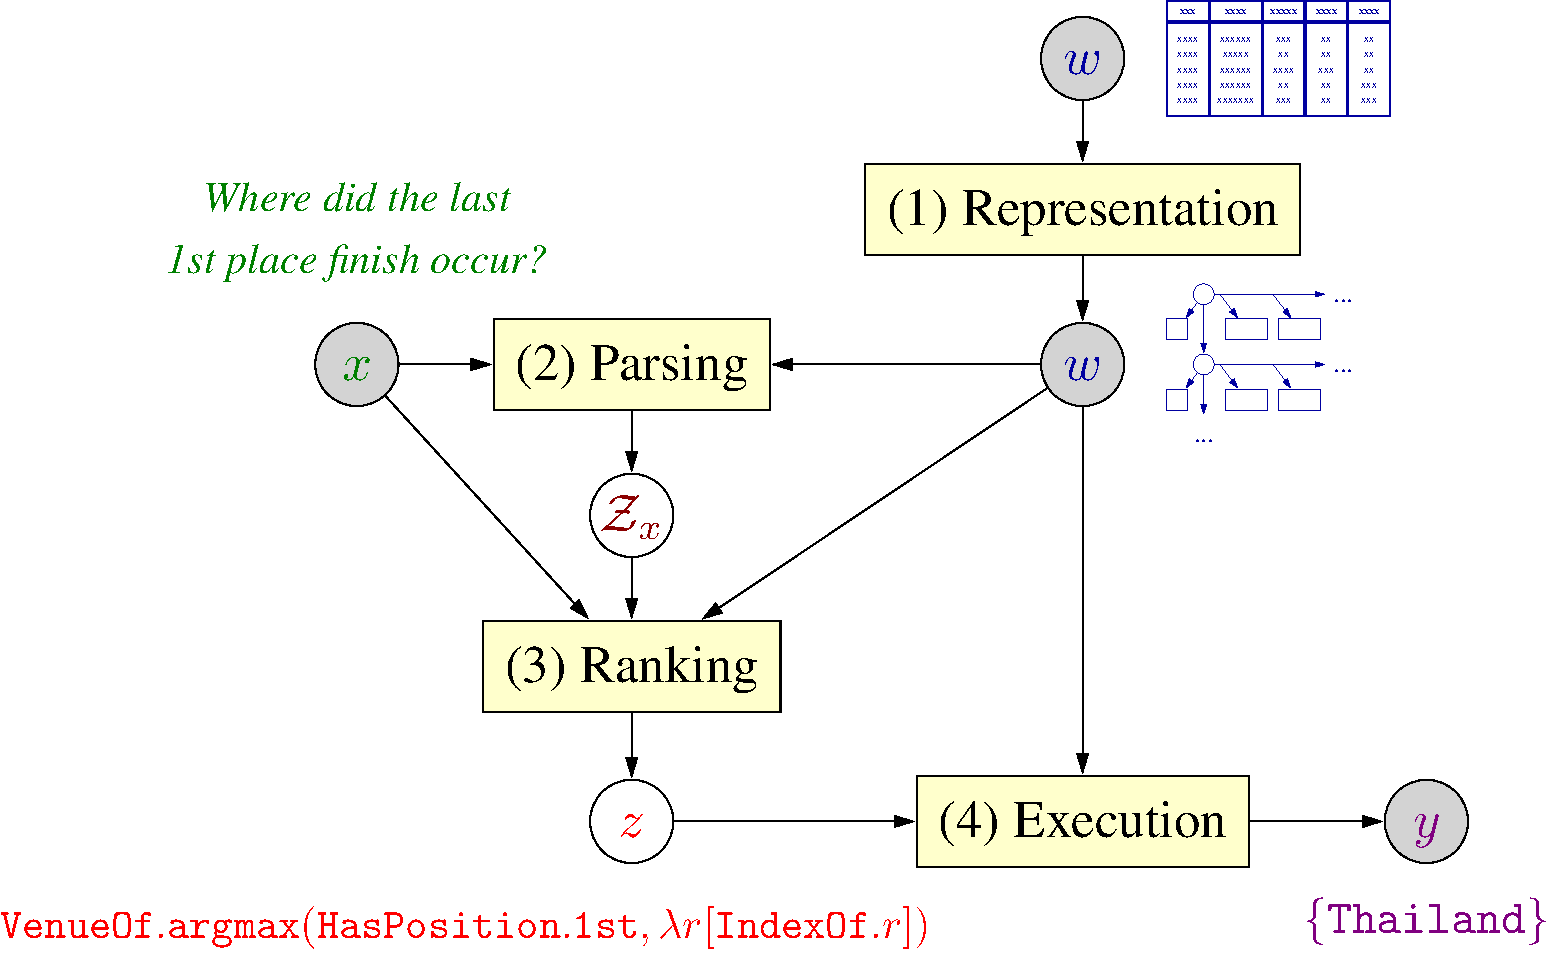
\includegraphics[scale=0.4]{sfig/sempre.slides/framework.pdf}
\caption[
The semantic parsing framework for answering questions
on web tables.
]{The semantic parsing framework for answering questions $x$
on web tables $w$.
At test time:
(1) the table $w$ is represented as a knowledge graph
as shown in Figure~\ref{fig:knowledge-graph};
(2) with information from $w$,
the question $x$ is parsed into candidate logical forms in $\zx$;
(3) the highest-scoring candidate $z\in\zx$ is chosen; and
(4) $z$ is executed on $w$, yielding the denotation $y$.
The model is trained to maximize the probability
of predicting the correct denotation.}
\label{fig:sempre-framework}
\end{figure}

\paragraph{Modeling.}
Given the question $x$ and a table $w$,
we use a logical form $z$
to represent the process for computing the answer $y$.
Formally,
we define a generative model
that generates $y$ from inputs $x$ and $w$
via a latent variable $z$.
Given a space $\Mc{Z}$ of \emph{all} possible logical forms,
we define a probability distribution
$p(z\mid x, w)$ over all $z \in \Mc{Z}$.
The probability of producing a denotation $y$ can be computed
by maginalizing over $z$:
\begin{equation}
p(y \mid x, w) =
\sum_{z \in \Mc{Z}}
\II(\deno{z}{w} = y)\,p(z \mid x, w)
\label{eqn:sempre-model}
\end{equation}
where $\deno{z}{w}$ is the denotation from executing
$z$ on $w$.

\paragraph{Prediction.}
Given a question $x$ on a table $w$,
we predict a logical form $z$ and an answer $y$
using an approximation of the generative model above.
Our prediction framework is illustrated in 
Figure~\ref{fig:sempre-framework}.
Since it is impossible to enumerate the set $\Mc{Z}$
of all possible logical forms,
we first generate a finite set of candidate logical forms
$\zx$ by parsing the question $x$ using the information
from the table $w$ (Section~\ref{sec:sempre-parsing}).
Each generated logical form $z \in \zx$
is associated with its denotation $y = \deno{x}{w}$
and a score $s_\theta(z, x, w)$,
where $s_\theta$ is a scoring function
(Section~\ref{sec:sempre-scoring})
with trainable parameters $\theta$.
We define a distribution over the candidate logical forms as
\begin{equation}
p_\theta(z \mid x, w) \propto \exp\crab{s_\theta(z, x, w)}.
\end{equation}
To predict $y$, we skip the marginalization over $z$
as written in Equation~\ref{eqn:sempre-model},
and instead just return the denotation of $z$
with the highest model probability $p_\theta(z\mid x, w)$
(or equivalently, the highest score $s_\theta(z, x, w)$).

\paragraph{Training.}
Given training data $\{(x\i, w\i, y\i)\}_{i=1}^N$,
we use a gradient ascent method to optimize $\theta$ to maximize
one of the following objective functions:

\begin{enumerate}
\item \emph{Log-likelihood of the correct denotations.}
To compute the log-likelihood of a denotation $y$,
we marginalize
over the logical forms $z \in Z_{x}$
that executes to $y$:
\begin{equation}
p_\theta(y \mid x, w) =
\sum_{z\in \zx} \II(\deno{z}{w} = y)\,p_\theta(z \mid x, w).
\end{equation}
The objective function is
\begin{equation}
J_\Mr{LL}(\theta) = 
\frac{1}{N} \sum_{i=1}^N \log p_\theta(y\i\mid x\i, w\i)
- \Omega(\theta)
\label{eqn:sempre-log-likelihood}
\end{equation}
where $\Omega$ is a regularization function.
Intuitively, a gradient update
will push up the scores of \emph{all}
consistent logical forms in $\zx$
(i.e., the ones with the correct denotation),
and push down the scores of \emph{all}
inconsistent logical forms in $\zx$.

A few previous studies have used
the log-likelihood object to train a semantic parser
\cite{kwiatkowski11lex,liang11dcs,berant2013freebase}.
While this objective function correctly maximizes
the marginalized probability of $y\i$,
it does not match the prediction process,
which does not marginalize over $z$.

\item \emph{Contrastive loss.}
From $\zx$,
we pick a logical form $z_+$
with the highest model probability among consistent
logical forms (i.e., logical forms giving the correct denotation),
and another logical form $z_-$ with the highest
probability among inconsistent logical forms.
The objective function is defined as
\begin{equation}
J_\Mr{cnt}(\theta) =
\frac{1}{N} \sum_{i=1}^N \log
\frac{p_\theta(z\i_+\mid x\i, w\i)}{p_\theta(z\i_-\mid x\i, w\i)}
- \Omega(\theta)
\end{equation}
Intuitively, a gradient update
will push up the scores of \emph{one}
consistent logical forms
and push down the scores of \emph{one}
inconsistent logical forms.
Unlike the usual contrastive loss
used in previous semantic parsing work
\cite{zettlemoyer07relaxed,zettlemoyer09context},
we always update the parameter
even when the probability of $z_+$
already exceeds that of $z_-$.
\end{enumerate}

The next four sections give more details about
each component of our framework.
Section~\ref{sec:sempre-graph} describes
how we represent the table as a \emph{knowledge graph},
which aids logical form execution and
helps us maintain uncertainty
over possible interpretations of the table.
Section~\ref{sec:sempre-lf} describes the syntax and semantics
of \emph{lambda DCS}, our logical form language.
Afterward in Section~\ref{sec:sempre-parsing},
we look at how the
set $\zx$ of candidate logical forms is generated from the input.
Finally, Section~\ref{sec:sempre-scoring}
defines the scoring function $s_\theta(z, x, w)$.

%%%%%%%%%%%%%%%%%%%%%%%%%%%%%%%%%%%%%%%%%%%%

\section{Graph representation of the table}
\label{sec:sempre-graph}

\begin{figure}[tp]
\centering
\textsf{
\begin{tabular}{|c|c|c|c|c|} \hline
\textbf{Year} & \textbf{Venue} & \textbf{Position} & \textbf{Event} & \textbf{Time} \\ \hline
2001 & Hungary & 2nd & 400m & 47.12 \\
2003 & Finland & 1st & 400m & 46.69 \\
2005 & Germany & 11th & 400m & 46.62 \\
2007 & Thailand & 1st & relay & 182.05 \\
2008 & China & 7th & relay & 180.32 \\ \hline
\end{tabular}
}
\\[1em]
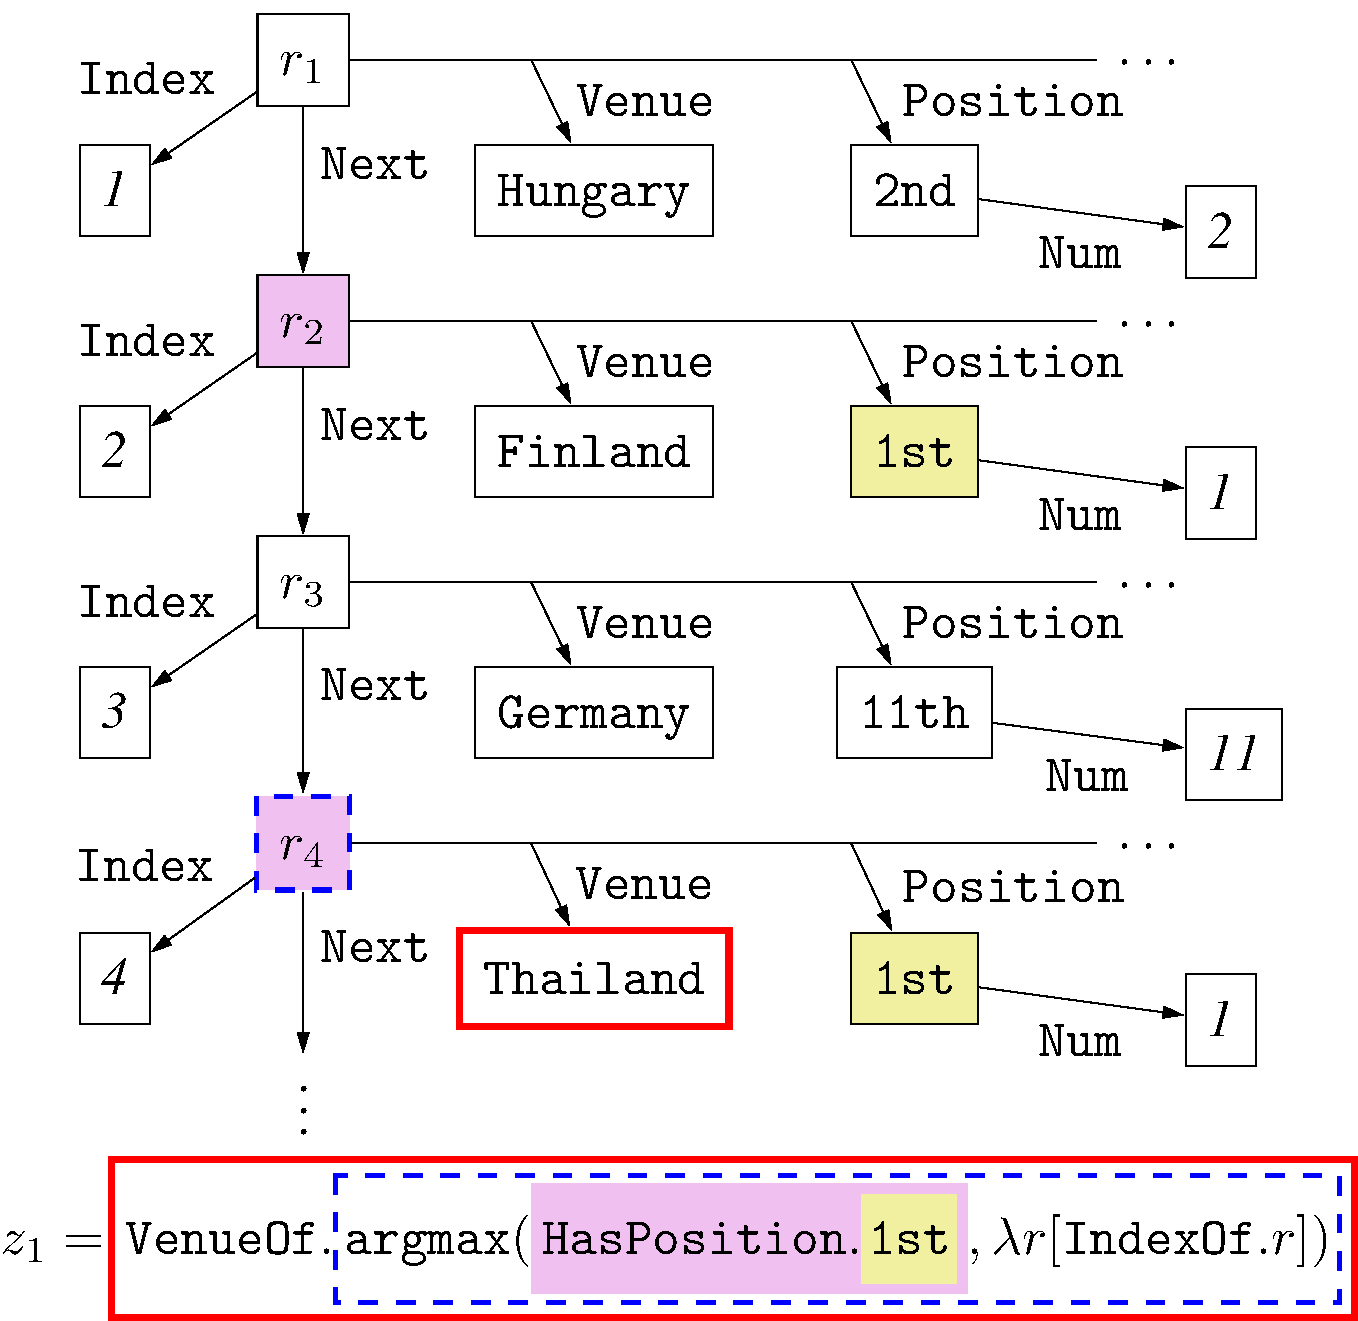
\includegraphics[scale=0.4]{sfig/dpd.slides/knowledgeGraph.pdf}
\caption[
Knowledge graph and execution of logical forms.
]{
The table $w$ is represented as a \emph{knowledge graph}.
The recursive execution of logical form $z$ is shown
via the different colors and styles.}
\label{fig:knowledge-graph}
\end{figure}

Inspired by the graph representation of knowledge bases,
we represent the table as a \emph{knowledge graph}
as illustrated in Figure~\ref{fig:knowledge-graph}.
The extensible graph structure
allows us to easily encode any additional information
by adding custom edges and nodes.
In particular, we will augment the graph with structures
for answering different types of questions
and maintaining uncertainty over different interpretations of the cell contents.

\paragraph{Basic construction.}
To construct a knowledge graph,
we first convert each row into a \emph{row node}
(e.g., the first row becomes $r_1$),
and convert cells into \emph{cell nodes}
(e.g., the cell with text \nl{Hungary}
becomes a node \T{Hungary}).
Then, we convert each column into directed \emph{column edges}
from the row nodes to the corresponding entity nodes
of that column,
and label the edges with the column header
(e.g., we construct an edge with label \T{Venue}
from $r_1$ to \T{Hungary}).
Note that columns are automatically renamed
to have unique texts if necessary.

\paragraph{Graph augmentation.}
One benefit of the graph representation
is that we can freely augment the graph with 
additional information that helps us answer the questions.

The first type of augmentation we employ is
\emph{normalization nodes}.
Some cell strings (e.g., \nl{2001})
can be interpreted as a number, a date, or a proper name
depending on the context,
while some other strings (e.g., \nl{200 km} and \nl{21-14})
have multiple parts.
Instead of committing to one normalization scheme,
we introduce normalization nodes for the possible ways
to interpret the cell strings,
and use special edges to link cell nodes to normalization nodes.
In this chapter, we consider two types of normalization:
\T{Num} (value of the first number in the cell)
and \T{Date} (year, month, and/or date that can be parsed from the cell).
For instance, a cell node \T{2001}
will have a \T{Num} edge pointing to the atomic value \C{2001.0},
and a \T{Date} edge pointing to the atomic value \C{2001-XX-XX}.

The second type of augmentation are row-specific edges.
Questions about tables usually involve reasoning about the
order of the rows. For instance,
\nl{What is the next \dots?} or \nl{Who came before \dots?}
require looking at adjacent rows,
while \nl{Who is the last \dots?} requires looking
at the last row among a group of rows.
To help answer these types of questions,
we augment each row node with an edge labeled \T{Next}
pointing to the next row node,
and an edge labeled \T{Index} pointing to the row index number
(starting from 1).

%%%%%%%%%%%%%%%%%%%%%%%%%%%%%%%%%%%%%%%%%%%%%%%

\section{Logical forms syntax and semantics}
\label{sec:sempre-lf}

\begin{table}[!p]
\centering
\begin{tabular}{lll@{}} \toprule
\textbf{Name} & \textbf{Logical form $z$} & \textbf{Denotation $\deno{z}{w}$} \\ \midrule
%
\textbf{Reverse}
& $\Mb{R}[b]$
& $\{(p, q) \mid (q, p) \in \deno{b}{w}\}$ \\
\example
& $\Mb{R}[\T{Venue}]$
& $\{(p, q) \mid q \too{Venue} p\}$ \\ \midrule
%
\textbf{Join}
& $b.u$
& $\{p \mid \exists q, q \in \deno{u}{w} \wedge (p, q) \in \deno{b}{w}\}$ \\
\addlinespace
\explainA{
\emph{Note:} To avoid confusion regarding the direction of Join,
we use the following notations when the binary $b$ is a graph edge:
$b.u$ is written as $\yHas{b}.u$, and $\Mb{R}[b].u$ is written as $\yOf{b}.u$.
} \\ \addlinespace
\example
& $\xHas{Year}.\T{2001}$
& $\{p \mid p \too{Year} \T{2001}\} = \{r_1\}$ \\
& $\xOf{Date}.\T{2001}$
& $\{p \mid \T{2001} \too{Date} p \} = \{\C{2001-XX-XX}\}$ \\
& $\xOf{Index}.\xHas{Position}.\T{1st}$
& $\{p \mid \exists q, q \too{Index} p \wedge q \too{Position} \T{1st}\}
= \{2, 4\}$ \\
& $\T{>=}.\C{4}$
& $\{p \mid p \geq 4\}$ \\ \midrule
%
\textbf{Union}
& $u_1 \sqcup u_2$
& $\{p \mid p \in \deno{u_1}{w} \vee p \in \deno{u_2}{w}\}$ \\
\example
& $\T{Finland} \sqcup \T{Hungary}$
& $\{\T{Finland}, \T{Hungary}\}$ \\ 
%
\textbf{Intersection}
& $u_1 \sqcap u_2$
& $\{p \mid p \in \deno{u_1}{w} \wedge p \in \deno{u_2}{w}\}$ \\
\example
& $\T{>=}.\C{1980} \sqcap \T{<}.\C{1990}$
& $\{p \mid 1980 \leq p < 1990\}$ \\ \midrule
%
\textbf{Aggregation}
& $A(u)$
& $\{p \mid p = A(\deno{u}{w})\}$ \\ \addlinespace
\explainA{Choices of the aggregation function $A$ include:} \\
\explainA{$\bullet$ \T{count}: number of elements in the set} \\
\explainA{$\bullet$ \T{min} and \T{max}: minimum and maximum value
(can only be used on a set of numbers or dates)} \\
\explainA{$\bullet$ \T{sum} and \T{avg}: sum and average value
(can only be used on a set of numbers)} \\ \addlinespace
\example
& $\T{count}(\xHas{Event}.\T{400m})$
& $\{p \mid p = \T{count}(\{q \mid q \too{Event} \T{400m}\})\} = \{3\}$ \\
\midrule
%
\textbf{Arithmetic}
& $\T{sub}(u_1, u_2)$
& $\{p\mid \exists q\exists q', q \in \deno{u_1}{w} \wedge q' \in \deno{u_2}{w} \wedge p = q - q'\}$ \\ \addlinespace
\explainA{For simplicity,
we only consider subtraction since other arithmetic operations are rare in our dataset.}
\\ \addlinespace
\example
& \multicolumn{2}{l}{$\T{sub}(\xOf{Index}.\xHas{Venue}.\T{China},
\xOf{Index}.\xHas{Venue}.\T{Hungary})$ \qquad $\{5 - 1\} = \{4\}$}
\\ \midrule
\textbf{Superlative}
& $\T{argmax}(u, b)$
& $\{p \mid p \in \deno{u}{w} \text{ such that for any other }
p' \in \deno{u}{w},$ \\
& \small{(\T{argmin} is defined similarly)}
& \quad$[\exists q \forall q', (q,p) \in \deno{b}{w} \wedge
(q',p') \in \deno{b}{w}
\Rightarrow q \geq q']\}$ \\ \addlinespace
\explainA{Intuitively,
the binary $b$ can be thought of as a function
mapping $p \in \deno{u}{w}$ to a set of values.
The \T{argmax} operator chooses the values $p$ that
give the maximum mapped value.}
\\ \addlinespace
\example
& $\T{allRows}$
& $\{r_1, r_2, r_3, r_4, r_5\}$ \\
& $\lambda r[\xOf{Index}.r]$
& $\{(1,r_1), (2,r_2), (3,r_3), (4,r_4), (5,r_5)\}$ \\
& $\T{argmin}(\T{allRows},
\lambda r[\xOf{Index}.r])$
& $\{r_1\}$ (giving the minimum value $1$)\\
& $\xHas{Position}.\T{1st}$ & $\{r_2, r_4\}$ \\
& \multicolumn{2}{l}{$\T{argmax}(\xHas{Position}.\T{1st}, \lambda r[\xOf{Index}.r])$ \qquad $\{r_4\}$} \\
\bottomrule
\end{tabular}

\caption[The syntax and semantics of lambda DCS logical operators.]
{The syntax and semantics of lambda DCS logical operators.
(Variables $u$ and $b$ denote a unary and a binary, respectively.
Variables $p$ and $q$ denote arbitrary values.)}
\label{tab:lambda-dcs-operators}
\end{table}

We use \emph{lambda dependency-based
compositional semantics} \cite{liang2013lambdadcs},
or \emph{lambda DCS},
as the language of our logical forms.
The language was originally designed for semantic parsing
on large knowledge graphs
\cite{berant2013freebase}.
As the context table can be converted into a knowledge graph
(Section~\ref{sec:sempre-graph}),
the lambda DCS formalism naturally transfers to our setting.

We now describe the syntax and semantics of lambda DCS constructs.
The knowledge graph in Figure~\ref{fig:knowledge-graph}
will be used as a running example.

\paragraph{Types of logical forms.}
A lambda DCS logical form is either a \emph{unary} or a \emph{binary}.
A unary represents a set of objects
(e.g., $\set{\T{Finland}, \T{Thailand}}$).
A binary represents a mapping from objects to objects,
which we will write as a set of pairs of objects
(e.g., $\set{(r_2, \T{Finland}), (r_4, \T{Thailand})}$).
We use $\deno{z}{w}$ to denote the denotation of $z$
with respect to the knowledge graph $w$
(i.e., the result of executing $z$ on $w$).

\paragraph{Primitives.}
Primitives are the smallest building blocks of lambda DCS logical forms.
Under the context of a knowledge graph $w$ from Section~\ref{sec:sempre-graph},
the primitive unaries are cell nodes
(e.g., $z = \T{Finland}$ with denotation $\deno{z}{w} = \set{\T{Finland}}$),
atomic values such as numbers and dates
(e.g., $z = \C{2001-XX-XX}$; $\deno{z}{w} = \set{\C{2001-XX-XX}}$),
and the special \T{allRows} symbol that executes
to the set of all row nodes (e.g.,
in our running example, $\deno{\T{allRows}}{w} = \{r_1, r_2, r_3, r_4, r_5\}$).

The primitive binaries are the graph edges
(e.g., $z = \T{Venue}; \deno{z}{w} = \set{(r_1, \T{Hungary}), (r_2, \T{Finland}), \dots}$)
and special binaries \T{=}, \T{!=}, \T{<}, \T{<=}, \T{>}, and \T{>=}
(e.g., $z = \T{<}$; $\deno{z}{w} = \set{(p, q) \mid p < q}$).

\paragraph{Operators.}
Larger logical forms can be constructed from smaller ones
using \emph{logical operators}.
Table~\ref{tab:lambda-dcs-operators}
lists the operators we use in our work.
Note that the direction of the binary
in our superlative operator (\T{argmax} and \T{argmin})
is the reverse of that in \citet{liang2013lambdadcs}.
This is to make the syntax more consistent
with the key-based comparison functions in many programming languages
(e.g., the logical form
$\T{argmax}(u, \lambda p[f(p)])$ is equivalent to
``\verb|max(u, key=lambda p: f(p))|'' in Python and
``\verb+u.max_by {|p| f(p)}+'' in Ruby).

\paragraph{Lambda abstraction.}
As seen in the examples of superlatives in
Table~\ref{tab:lambda-dcs-operators},
one way to construct more complex logical forms
is to use \emph{lambda abstraction}
to construct a binary.
For a logical form $f(p)$ containing a free variable $p$,
the construct $\lambda p[f(p)]$
is a binary with denotation
$\{(q, p) \mid q \in \deno{f(p)}{w} \}$.
For example, the binary
$\lambda p[\T{count}(\xHas{Event}.p)]$
counts the number of rows for each value in the \emph{Event}
column, and thus executes to
$\{(3, \T{400m}), (2, \T{Relay})\}$.\footnote{
Technically, the denotation also contains
$(0, p)$ for any other values $p$.}

\paragraph{Terminologies.}
Each token in a logical form is called a \emph{predicate}.
A logical form $z$ is \emph{consistent} with a value $y$
if its denotation $\deno{z}{w}$ matches $y$;
otherwise, it is \emph{inconsistent}.
Note that the matching can be done loosely to
get around text normalization issues
in the annotated answers
(e.g., a logical form whose denotation is $\{32\}$
is still treated as consistent with
the correct answer \nl{32 km}).

%%%%%%%%%%%%%%%%%%%%%%%%%%%%%%%%%%%%%%%%%%%%%%%

\section{Parsing the utterance into logical forms}
\label{sec:sempre-parsing}

Given a knowledge graph $w$,\footnote{
We overload the variable $w$ for both the table and
its knowledge graph representation.
Clarification will be made when necessary.}
we want to parse the input question $x$
and generate a set $\zx$ of candidate logical forms.
This section describes a bottom-up semantic parser
that produce the logical forms and their scores.

\subsection{Deduction rules}
The space of possible logical forms given the knowledge graph $w$
and the question $x$ is defined recursively
by a set of \emph{deduction rules},
which dictate how logical forms
can be constructed either from the inputs
or from smaller logical forms
\cite{zettlemoyer07relaxed,berant2013freebase}.
Informally,
our parser
maintains a set of logical forms,
and then repeatedly applies deduction rules
to construct larger logical forms
from smaller ones in the set.
Logical forms that are ``well-formed''
are finally compiled into
the set $\zx$ of candidate logical forms.
The parsing algorithm will be described more formally
in Section~\ref{sec:floating-parser}.

Deduction rules are divided into two types: terminal rules
and compositional rules.

\paragraph{Terminal rules.}
A terminal rule creates logical forms based on the input
question $x$ and knowledge graph $w$.
Each terminal rule follows one of the following templates:
\begin{align}
\C{TokenSpan}[s] &\to c[f(s)] \label{eqn:rule-b1} \\
\varnothing &\to c[f()] \label{eqn:rule-b2}
\end{align}

A rule of Template~\ref{eqn:rule-b1} takes
a token span from the question $x$
and applies the \emph{semantic function} $f$,
which generates a set of logical forms.
The resulting logical forms will be associated with
a \emph{category} $c$, which is used to enforce type consistency.
For instance, let $\mathrm{match}$ be a function
that takes a string $s$
and returns cell nodes whose cell content strings
match $s$.
Then the deduction rule
\begin{equation}
\C{TokenSpan}[s] \to \C{Entity}[\mathrm{match}(s)]
\end{equation}
can construct logical forms of category \C{Entity}
by applying the function $\mathrm{match}$
on some token span $s$ of $x$.

A rule of Template~\ref{eqn:rule-b2} works similarly,
but does not require any string from the question $x$.
Apart from generating input-independent logical forms
(e.g., \T{>=}\, and \T{allRows}),
this template is also useful when the logical form
is difficult to infer deterministically from the question.
For example, in most questions,
the relevant column names are indirectly mentioned
or implicitly implied
(e.g., the question \runningEx
in Figure~\ref{fig:sempre-running-ex}
indirectly mentions the columns \T{Venue} and \T{Position}).
We can use the following deduction rule
to generate such columns from the table:
\begin{equation}
\varnothing \to \C{Relation}[\mathrm{columns}()],
\end{equation}
where the function $\mathrm{columns}$ returns all unique column edges
from the knowledge graph $w$.

\paragraph{Compositional rules.}
A compositional rule constructs larger logical forms
from smaller ones.
Each compositional rule follows one of the following templates:
\begin{align}
c_1[z_1] &\to c[g(z_1)] \label{eqn:rule-c1} \\
c_1[z_1] + c_2[z_2] &\to c[g(z_1, z_2)] \label{eqn:rule-c2}
\end{align}

A rule of Template~\ref{eqn:rule-c1}
takes a child logical form $z_1$ of category $c$,
and then constructs a new logical form $g(z_1)$ of category $c$.
For instance, if $g(z_1) = \T{count}(z_1)$,
we can construct
$\T{count}(\xHas{Position}.\T{1st})$
from an existing logical form $\xHas{Position}.\T{1st}$.
A rule of Template~\ref{eqn:rule-c2}
operates similarly but takes two children logical forms.

\begin{table}[tb]\centering
\begin{tabular}{@{\;}r@{ $\to$ }lll@{}} \toprule
\multicolumn{2}{c}{\textbf{Rule}} & \textbf{Semantics}
& \textbf{Example} \\ \midrule

$\C{TokenSpan}$ & $\C{Entity}$
& $\mathrm{match}(s)$
& $\T{Finland}$ \\
\explainB{cell node with string $s$}
&from \emph{``Finland''} \\

$\C{TokenSpan}$ & $\C{Atomic}$
& $\mathrm{value}(s)$
& $\C{2012-07-XX}$ \\
\explainB{interpretation of $s$ at an atomic value} 
&from \emph{``July 2012''} \\

\midrule

\multicolumn{2}{l}{\quad$\varnothing$ $\to$ $\C{Relation}$}
& $\mathrm{columns}()$
& $\T{Venue}$ \\
\explainB{all column edges} \\

\multicolumn{2}{l}{\quad$\varnothing$ $\to$ $\C{Relation}$}
& $\mathrm{normalizedColumns}()$
& $\lambda x[\xHas{Year}.\xHas{Date}.x]$ \\
\explainBLong{binaries formed by joining a column edge with
a normalization edge} \\

\multicolumn{2}{l}{\quad$\varnothing$ $\to$ $\C{Records}$}
& $\T{allRows}$ \\

\multicolumn{2}{l}{\quad$\varnothing$ $\to$ $\C{RecordFn}$}
& $\lambda r.[\xOf{Index}.r]$ \\

\bottomrule

\end{tabular}
\caption[Terminal deduction rules.]{
Terminal deduction rules.
Entities and atomic values (numbers and dates) are constructed from
token spans while other predicates are not.
}\label{tab:sempre-terminal-rules}
\end{table}

%%%%%%%%%%%%%%%%%%%%%%%%%%%%%%%%%%%%%%%%%%%%%%%

\begin{table}[tb]\centering\small
\begin{tabular}{@{\;}r@{ $\to$ }lll@{\;}} \toprule
\multicolumn{2}{c}{\textbf{Rule}} & \textbf{Semantics}
& \textbf{Example} \\ \midrule

\multicolumn{4}{c}{\textbf{\emph{Join + Aggregate}}} \\ 

$\C{Entity}$ or $\C{Atomic}$ & $\C{Values}$
& $z_1$
& $\T{Finland}$ \\

$\C{Atomic}$ & $\C{Values}$
& $c.z_1$
& $\T{>=}.\C{30}$ \\
\explainB{$c \in \{\T{<}, \T{>}, \T{<=}, \T{>=}\}$} \\

$\C{Relation} + \C{Values}$ & $\C{Records}$
& $z_1.z_2$
& $\xHas{Venue}.\T{Finland}$ \\

$\C{Relation} + \C{Records}$ & $\C{Values}$
& $\Mb{R}[z_1].z_2$
& $\xOf{Year}.(\xHas{Venue}.\T{Finland})$ \\

$\C{Records}$ & $\C{Records}$
& $\xHas{Next}.z_1$
& $\xHas{Next}.(\xHas{Venue}.\T{Finland})$ \\

$\C{Records}$ & $\C{Records}$
& $\xOf{Next}.z_1$
& $\xOf{Next}.(\xHas{Venue}.\T{Finland})$ \\

$\C{Values}$ & $\C{Atomic}$
& $A(z_1)$
& $\T{count}(\xHas{Venue}.\T{Finland})$ \\
\explainB{$A \in \{\T{count}, \T{max}, \T{min}, \T{sum}, \T{avg}\}$} \\

$\C{Values}$ & $\C{ROOT}$
& $z_1$ \\

\midrule

\multicolumn{4}{c}{\textbf{\emph{Union + Intersection}}} \\

$\C{Entity} + \C{Entity}$ & $\C{Values}$
& $z_1 \sqcup z_2$
& $\T{Finland} \sqcup \T{Germany}$ \\

$\C{Records} + \C{Records}$ & $\C{Records}$
& $z_1 \sqcap z_2$
& $\xHas{Position}.\T{1st} \sqcap \xHas{Event}.\T{Relay}$ \\

\midrule

\multicolumn{4}{c}{\textbf{\emph{Superlative over rows}}} \\ 

\explainBLong{A \C{RecordFn} $\lambda r[f(r)]$
is a function that maps row nodes $r$ into comparable values} \\

$\C{Relation}$ & $\C{RecordFn}$
& $\lambda r[\Mb{R}[z_1].r]$
& $\lambda r[\xOf{Num}.\xOf{Time}.r]$ \\

$\C{Records} + \C{RecordFn}$ & $\C{Records}$
& $S(z_1, z_2)$
& $\T{argmax}(\T{allRows}, \lambda r[\xOf{Num}.\xOf{Time}.r])$ \\

\explainB{$S \in \{\T{argmax}, \T{argmin}\}$} 
& $\T{argmin}(\xHas{Position}.\T{1st}, \lambda r[\xOf{Index}.r])$ \\

\midrule

\multicolumn{4}{c}{\textbf{\emph{Arithmetic}}} \\

\explainBLong{A \C{ValueFn} $\lambda v[f(v)]$
is a function that maps values $v$ (cells or atomic values)
into comparable values} \\

$\C{Relation}$ & $\C{ValueFn}$
& $\lambda v[A(z_1.v)]$
& $\lambda v[\T{count}(\xHas{Event}.v)]$  \\

$\C{Relation} + \C{Relation}$ & $\C{ValueFn}$
& $\lambda v[\Mb{R}[z_1].z_2.v]$
& $\lambda v[\xOf{Num}.\xOf{Time}.\xHas{Event}.v]$ \\

{\scriptsize$\C{ValueFn} + \C{Values} + \C{Values}$}
& $\C{Values}$
& \hspace*{-1em}{$\T{sub}(z_1.z_2, z_1.z_3)$}
& $\T{sub}(\T{count}(\xHas{Event}.\T{400m}), \T{count}(\xHas{Event}.\T{Relay}))$ \\

\bottomrule

\end{tabular}
\caption[Compositional deduction rules.]{
Compositional deduction rules.
Each rule $c_1, \dots, c_k \to c$ takes logical forms $z_1, \dots, z_k$
constructed over categories $c_1, \dots, c_k$, respectively,
and produces a logical form based on the semantics.
}\label{tab:sempre-compositional-rules}
\end{table}

\paragraph{List of deduction rules.}
Tables~\ref{tab:sempre-terminal-rules}~and~\ref{tab:sempre-compositional-rules}
detail the deduction rules used in our parser.
The deduction rules are designed to be closely mimic
the compositional syntax of lambda DCS.
However, as some lambda DCS constructs are very generic
and can generate many nonsensical logical forms
(e.g., the subtraction operator can subtract
any two arbitrary numbers),
some operators are restricted to be applied
only in certain contexts
(e.g., only allow subtracting numbers from two cells
from the same column).
This trade-off prevents us from
answering some small number of sophisticated questions,
but we found it necessary for making the space
of generated logical forms manageable.

From the table,
we can see that many deduction rules
construct logical forms
without referencing the question.
These include the terminal rules of the form
$\varnothing \to c[f()]$
and various compositional rules
that generate operators
(e.g., \T{argmax} can be generated even when
the question does not have any word that expresses superlative).
This is intentional for two reasons:
\begin{itemize}
\item Many logical form predicates do not explicitly align
to any token from the question.
\item Even when the alignment exist, we want to learn
such an alignment from the data.
This will be achieved by the features in the scoring module
that relate logical form predicates to the tokens in the question.
\end{itemize}

\subsection{Floating parser}\label{sec:floating-parser}
To parse the question $x$ based on the deduction rules,
we propose a new parser named \emph{floating parser}
that can construct logical forms in a flexible order.

\paragraph{Chart parser.}
To understand the motivation behind the floating parser,
let us first consider a more common bottom-up parsing algorithm:
the CKY algorithm for chart parsing.

Given an input sentence $x$ with tokens $x_1, \dots, x_n$,
the algorithm constructs and stores partial parses
with category $c$
of the token span $x_{i:j} := (x_i, \dots, x_{j-1})$
in a \emph{cell} labeled $(c, i, j)$.
Being a dynamic programming algorithm,
the CKY algorithm populates the cells in the increasing order
of their span lengths $j - i$.
To construct a parse for the cell $(c, i, j)$,
we have the following choices:
\begin{itemize}
\item Apply a terminal rule of the form
\begin{equation*}
\C{TokenSpan}[s] \to c[f(s)]
\end{equation*}
on the token span $s = x_{i:j}$ to get logical forms $z \in f(s)$.
\item Apply a compositional rule of the form
\begin{equation*}
c_1[z_1] + c_2[z_2] \to c[g(z_1, z_2)]
\label{eqn:rule-c2-again}
\end{equation*}
on $z_1$ from cell $(c_1, i, k)$ and
$z_2$ from cell $(c_2, k, j)$ (for some $k \in \set{i,\dots,j-1}$)
to get a logical form $z = g(z_1, z_2)$
\item Apply a compositional rule of the form
\begin{equation*}
c_1[z_1] \to c[g(z_1)]
\end{equation*}
on another logical form $z_1$ from the same cell $(c, i, j)$
to get $z = g(z_1)$.
To avoid an infinite loop,
one can either design the deduction rules
to not have loops,
or use heuristics to detect and stop loops.
\end{itemize}

In any case, the parse is an abstract object containing
the constructed logical form $z$, plus any other metadata necessary
to score the logical form (e.g., when applying
Rule~\ref{eqn:rule-c2-again}, we can store the child parses
where $z_1$ and $z_2$ come from).
To restrict the search space to a reasonable size,
\emph{beam search} is usually employed:
the populated cells are pruned down to some
fixed number of parses that have the highest scores.
The parses in cell $(\C{ROOT}, 0, n)$
form the set $\zx$ of final logical forms.

\paragraph{Challenges.}
Chart parsing found success in syntactic parsing,
where all words end up participating in the parse,
and the parse forms a proper tree with no reordering.
In contrast, for our semantic parsing task,
the chart parser is restrictive for several reasons:
\begin{itemize}
\item
While each parse in chart parsing belongs
to some token span $x_{i:j}$,
some semantic predicates do not naturally align
to a token.
Consider the following question on a table about
Olympic games:
\begin{center}
\nl{Greece held its last Summer Olympics in which year?} \\
$\xOf{Date}.\xOf{Year}.\T{argmax}(\xHas{Country}.\T{Greece}, \lambda r[\xOf{Index}.r])$
\end{center}
While the cell node \T{Greece} can be generated from
the word \nl{Greece}, some logical form predicates
such as \T{Country} cannot be aligned to a token span.
We could potentially learn to generate the whole
$\xHas{Country}.\T{Greece}$ from \nl{Greece},
but this requires writing more custom deduction rules.
\item
Conversely, some token does not align with
a semantic predicate.
In the example above, \nl{Summer} and \nl{Olympics}
do not manifest in the logical form.
\item
Finally, the order of question tokens
and the logical form predicates
may not align well.
In the example above,
the word \nl{year} comes last,
but the predicate \T{Year} comes first.
\end{itemize}

Previous semantic parsing work
addresses the challenges above by
using a \emph{lexicon}
that maps utterance phrases
to corresponding logical form fragments
\cite{zettlemoyer07relaxed,kwiatkowski10ccg,kwiatkowski11lex,berant2013freebase}.
The lexicon can either be manually specified
or jointly learned with the parser.
However, with an open-domain knowledge source with unknown data schema,
such as a random web table,
the lexicon is unlikely to have coverage over
the unseen relations.

We instead opt for a more general solution:
we allow some predicates to be constructed from other sources
than the utterance.
The relation between the utterance and the predicate
is instead softly captured by the scoring function.
As a result, our \emph{floating parser}
can achieve a high coverage over logical forms
even for tables with unseen data schema.

\paragraph{Floating parser.}
As motivated above,
the floating parser does not require logical form predicate to
be constructed from utterance tokens.
We replace the cells $(c, i, j)$,
with \emph{floating cells} $(c, s)$,
which will store logical forms
of category $c$ that have size $s$.
The size is measured as the number of compositional rules applied
during the construction of the logical form,
and not the number of logical form predicates.

The deduction rules now operate as follows:
\begin{itemize}
\item A terminal rule of the form
\begin{equation*}
\C{TokenSpan}[s] \to c[f(s)]
\end{equation*}
constructs $z \in f(s)$ in cell $(c, 0)$.
\item A terminal rule of the form
\begin{equation*}
\varnothing \to c[f()]
\end{equation*}
constructs $z \in f()$ in cell $(c,0)$.
This allows logical form predicates to be generated
out of thin air.
\item A compositional rule of the form
\begin{equation*}
c_1[z_1] + c_2[z_2] \to c[g(z_1, z_2)]
\end{equation*}
takes $z_1$ from cell $(c_1, s_1)$ and
$z_2$ from cell $(c_2, s_2)$
to construct $z = g(z_1, z_2)$
in cell $(c, s_1 + s_2 + 1)$.
\item A compositional rule of the form
\begin{equation*}
c_1[z_1] \to c[g(z_1)]
\end{equation*}
takes $z_1$ from cell $(c_1, s_1)$ 
to construct $z = g(z_1)$ in cell $(c, s_1 + 1)$.
\end{itemize}

\begin{figure}[t]
\centering
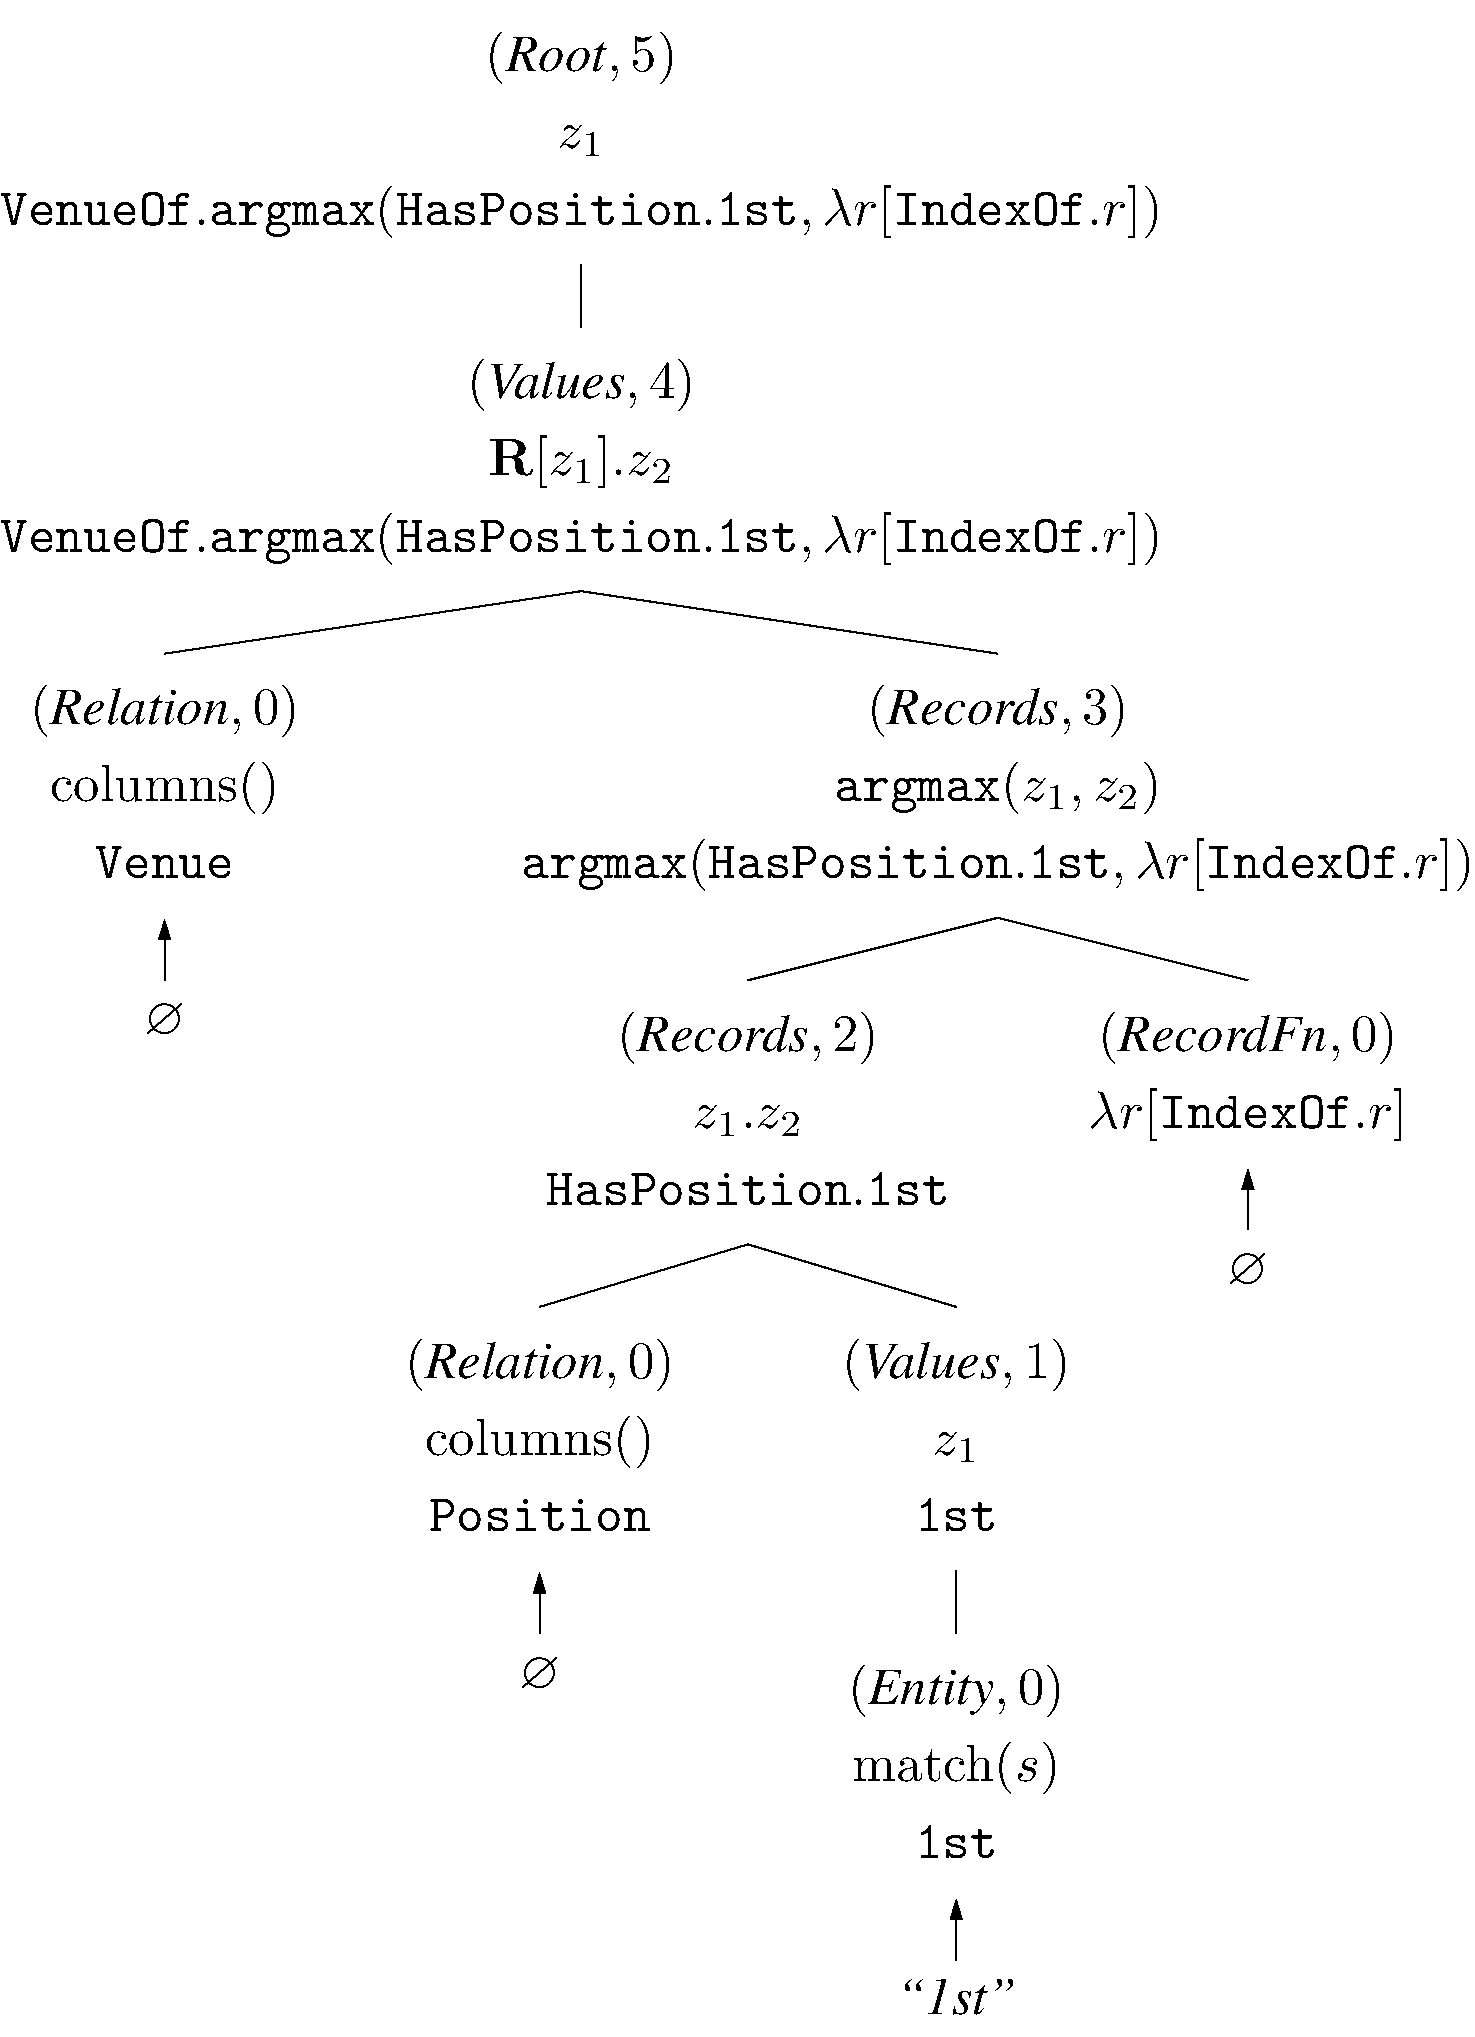
\includegraphics[scale=0.35]{sfig/parsetrees.slides/baseParse.pdf}
\caption[Derivation tree of the running example.]
{A derivation tree for the utterance \runningEx.
Each tree node shows the cell $(c,s)$,
the semantic function used,
and the resulting logical form.
Among the terminal rule applications (indicated by arrows),
only $\T{1st}$ is generated from a phrase \nl{1st} using the $\Mr{match}$ function;
other predicates are not generated based on the utterance.}
\label{fig:floating-parse-ex}
\end{figure}

Figure~\ref{fig:floating-parse-ex} shows
an example parse generated by our floating parser.
After populating the cells up to some maximum size $s = s_\Mr{max}$,
the parses in cell $(\C{ROOT}, s)$ for all sizes $s$
are compiled into the set $\zx$ of final logical forms.

\paragraph{Pruning.}

The floating parser is very flexible:
it can skip tokens,
generate tokens out of thin air,
and combine logical forms in any order.
This flexibility might seem too unconstrained,
but we can use several techniques to prevent
bad logical forms from being constructed:

\begin{itemize}
\item \textbf{Denotation-based pruning.}
Constructed logical forms can be executed
on the knowledge graph $w$ to get denotations.
We prune logical forms that execute to an empty set
(e.g., $\xHas{Year}.\xHas{Num}.\C{1}$).
While it is tempting to prune logical forms that do not execute,
care must be taken since some constructed logical forms
are partial and are meant to be used as an argument
of a larger logical form
(e.g., logical forms of category \C{ValueFn}
are meant to be used in superlative logical forms).

\begin{table} \centering
\begin{tabular}{ll} \toprule
\textbf{Criterion for pruning a logical form $z$} & \textbf{Example} \\ \midrule
% emptyDenotation + nonLambdaError
$z$ cannot be executed or executes to an empty set
& $\xHas{Venue}.\T{1st}$ \\
% forwardBackward
$z$ contains a relation joined with its inverse
& $\xOf{Position}.\xHas{Position}.\T{1st}$ \\
% doubleNext
$z$ contains a join of two $\T{Next}$ predicates
& $\xOf{Next}.\xOf{Next}.\xHas{Position}.\T{1st}$ \\
% sameMerge
$z$ is a union or intersection of identical logical forms
& $\T{1st} \sqcap \T{1st}$ \\
% mistypedMerge
$z$ is a union or intersection of values with different types
& $\T{5th} \sqcup \T{Germany}$ \\
\quad (Cells from different columns are considered different types.) \\
% badSuperlativeHead
$z$ is a superlative on a set of size 1
& $\T{argmax}(\xHas{Index}.\C{1}, \dots)$ \\
% multipleSuperlatives
$z$ contains multiple superlatives
& $\T{argmax}(\dots) \sqcap \T{argmin}(\dots)$ \\
% singleton
$z$ is a \C{ROOT} logical form with only a single predicate
& $\T{1st}$ (at category \C{ROOT})\\
% tooManyValues
$z$ is a \C{ROOT} logical form whose denotation contains > 10 values \\
\bottomrule
\end{tabular}
\caption{Heuristics for controlling the search space of the floating parser.}
\label{tab:sempre-heuristics}
\end{table}

\item \textbf{Heuristic pruning.}
Some logical forms can be properly executed,
but are unlikely to be relevant for answering the questions.
For instance, a union of objects from different columns
(e.g., $\T{5th} \sqcup \T{Germany}$)
are less likely to be reflecting what the question asks.
We use several heuristics listed in Table~\ref{tab:sempre-heuristics}
to prune logical forms.
Note that some heuristics could potentially prevent us
from answering some questions
(e.g., preventing joining two \T{Next} predicates
could prevent us from answering
\nl{What comes before the person before \dots?}).
However, these questions are rare enough,
and pruning these patterns would prune a large portion of the
search space, which increases speed and prevents overfitting
to incorrect logical form patterns.

\item \textbf{Score-based pruning (beam search).}
Even with the pruning strategies above,
the set of possible logical forms in each set
might still be large.
To control the search space,
we employ beam search by scoring the logical forms
and only keep the $B = 50$
highest-scoring logical forms in each cell.

\end{itemize}

\section{Scoring logical forms}\label{sec:sempre-scoring}

\begin{table}[t]\centering
\textsf{
\begin{tabular}{|c|c|c|c|c|} \hline
\textbf{Year} & \textbf{Venue} & \textbf{Position} & \textbf{Event} & \textbf{Time} \\ \hline
2001 & Hungary & 2nd & 400m & 47.12 \\
2003 & Finland & 1st & 400m & 46.69 \\
2005 & Germany & 11th & 400m & 46.62 \\
2007 & Thailand & 1st & relay & 182.05 \\
2008 & China & 7th & relay & 180.32 \\ \hline
\end{tabular}
} \\[.5em]
$x = \text{\nl{The last 1st place finish is in which year?}}$ \\
$z = \xOf{Num}.\xOf{Year}.\T{argmax}(\T{allRows}, \lambda r[\xOf{Index}. r])$ \\
$y = \{\C{2008}\}$
(type: \Sc{Num}, column: \T{Year}) \\[.5em]
\begin{tabular}{ll} \toprule
\textbf{Feature Name} & \textbf{Note} \\ \midrule
\textbf{phrase-predicate} \\
$\text{phrase} = \text{\nl{last}}, \text{predicate} = \T{argmax}$
& lexicalized \\
$\text{phrase} = \text{predicate}, \text{type} = \text{relation}$
& unlexicalized ($\because \text{\nl{year}} = \T{Year}$) \\
\midrule
\textbf{missing-predicate} \\
missing entity & unlexicalized ($\because$ missing \nl{1st}) \\
\midrule
\textbf{denotation} \\
$\text{denotation type} = \Sc{Num}$ \\
$\text{denotation column} = \Sc{Year}$ \\
\midrule
\textbf{phrase-denotation} \\
$\text{phrase} = \text{\nl{which year}}, \text{denotation type} = \Sc{Num}$
& lexicalized \\
$\text{phrase} = \text{denotation column}$
& unlexicalized ($\because \C{``year''} = \T{Year}$) \\
\midrule
\textbf{headword-denotation} \\
$Q = \text{\nl{which}}, \text{denotation type} = \Sc{Num}$
& lexicalized \\
$H = \text{\nl{year}}, \text{denotation type} = \Sc{Num}$
& lexicalized \\
$H = \text{denotation column}$ & unlexicalized ($\because \text{\nl{year}} = \T{Year}$) \\
\bottomrule
\end{tabular}
\caption[
Example features defined by our floating parser
]{
Example features defined
for the (incorrect) logical form $z$.
All features are binary features.
}\label{tab:features-ex}
\end{table}

Each logical form $z$ is associated with a score $s_\theta(z, x, w)$.
We adopt a linear model with features that capture the relationship
between the question $x$ and the logical form.
Concretely,
\begin{equation}
s_\theta(z, x, w) := \theta^\top \phi(z, x, w)
\end{equation}
where $\phi(z, x, w)$ is a feature vector.
Table~\ref{tab:features-ex}
shows example features from each feature type
described below:

\begin{itemize}

\item \textbf{phrase-predicate}:
For each n-gram $p_\Mr{x}$ from the question $x$
(up to 3-grams)
and a predicate $p_\Mr{z}$ from $z$,
we define a lexicalized
indicator feature
``$\text{phrase} = p_\Mr{x}, \text{predicate} = p_\Mr{z}$''.
These features capture the correspondence between
phrases and either close-classed predicates
(e.g., \nl{last} correlates with \T{argmax})
or frequent context-dependent predicates
(e.g., \nl{when} correlates with \T{Year}).

Additionally,
to handle open-domain predicates from the table,
we define an unlexicalized feature
``$\text{phrase} = \text{predicate}$''
when the phrase $p_\Mr{x}$ matches the string form of $p_\Mr{z}$.
The unlexicalized features can also have more specific details
based on substring matching,
part-of-speech tag of the phrase,
and the predicate type
(e.g., ``$\text{phrase} = \text{suffix of predicate}, \text{POS} = \text{W N}, \text{predicate type} = \text{entity}$'').

\item \textbf{missing-predicate}:
We define unlexicalized indicator features ``missing entity''
and ``missing relation''
when there are entities or relations mentioned in $x$
that are not present in $z$.

\item \textbf{denotation}:
From the denotation $y = \deno{z}{w}$,
we use its size (i.e., number of elements in the set $y$)
and its type to define unlexicalized features.
The type can be a primitive type (e.g., \Sc{Num}, \Sc{Date})
or the column containing the values in $y$
in case those values are cells.

\item \textbf{phrase-denotation}:
For each n-gram $p_\Mr{x}$ from the question $x$,
we define a lexicalized feature
``$\text{phrase} = p_\Mr{x}, \text{denotation type} = p_\Mr{y}$''
where $p_\Mr{y}$ is the type of $y$.
Like the phrase-predicate features,
we also define an unlexicalized feature
``$\text{phrase} = \text{denotation column}$''
when the type $p_\Mr{y}$ is a column whose string matches $p_\Mr{x}$.
Like phrase-predicate features, the unlexicalized feature
can be refined by substring match and part-of-speech tags.

\item \textbf{headword-denotation}:
From the part-of-speech tags of the question $x$,
we deterministically identify the question word $q_\Mr{x}$
(e.g., \emph{who}, \emph{when}, \emph{what})
and the head word $h_\Mr{x}$
(the first noun after the question word).
We then define lexicalized features
joining ``$\text{denotation type} = p_\Mr{y}$''
with ``$Q = q_\Mr{x}$'', ``$H = h_\Mr{x}$'', or both.
We also define unlexicalized features if $q_\Mr{x}$ or $h_\Mr{x}$
matches the column string of the denotation.

\end{itemize}

\section{Experiments}
We develop our model on three 80:20 splits
of the training portion of the \wtq dataset (14,152 examples),
where we report the average of three evaluation scores.
For the final evaluation,
we train on the training portion and 
test on the ``unseen'' test portion
(4,345 examples).

\subsection{Main evaluation}
The main evaluation metric is \emph{accuracy}:
the fraction of test examples where
the parser predicts the correct denotation
(in other words, the highest-ranking logical form is consistent
with the correct answer).
We also report the \emph{oracle} score:
the fraction of test examples where
the at least one of the logical forms in the
final candidate list $\zx$ is consistent with the correct answer.

\paragraph{Model details.}
We train the model using AdaGrad \cite{duchi10adagrad}
with an initial learning of 1.0.
For the experiments in this chapter,
we use the log-likelihood objective
(Equation~\ref{eqn:sempre-log-likelihood})
and lazy L1 regularization
with coefficient 0.001.
We take 3 passes over the training data.
The beam size is set to $B = 200$.

\paragraph{Baselines.}
We compare our systems to two baselines:
\begin{itemize}

\item \textbf{Information retrieval baseline (IR)}:
The IR baseline selects a cell $y$
among the table cells by applying a log-linear model
over the cells.
The features are conjunctions of the phrases of $x$
and the properties of $y$,
which covers all features of our parser
that do not depend on the logical form.

\item \textbf{\Sc{WebQuestions} baseline (WQ)}:
We restrict the logical form operators to the ones
present in the previous semantic parsing work
on the \Sc{WebQuestions} dataset
\cite{berant2013freebase}.
This includes the join and \T{count} operators.
\end{itemize}

\begin{table}[t]\centering
\begin{tabular}{lrrrr} \toprule
& \multicolumn{2}{c}{\textbf{dev}}
& \multicolumn{2}{c}{\textbf{test}} \\
\cmidrule(r){2-3} \cmidrule(l){4-5}
& \textbf{acc} & \textbf{ora} & \textbf{acc} & \textbf{ora} \\ \midrule
IR baseline & 13.4 & 69.1 & 12.7 & 70.6 \\
WQ baseline & 23.6 & 34.4 & 24.3 & 35.6 \\
Floating parser & 37.0 & 76.7 & 37.1 & 76.6 \\
\bottomrule
\end{tabular}
\caption[
Accuracy and oracles scores on
development and test data.
]{
Accuracy (acc) and oracle scores (ora) 
on the development sets
(3 random splits of the training data)
and the test data.}
\label{tab:sempre-results}
\end{table}

\paragraph{Main results.}
Table~\ref{tab:sempre-results}
shows the accuracy and oracle scores
of the floating parser and the baseline systems.
Our parser outperforms the baselines
by a significant margin.
In the following sections,
we use one of the development splits of the training data
to analyze various aspects of the \wtq dataset
and the floating parser.

\subsection{Error analysis}
\label{sec:sempre-error-analysis}

The error on the development data can be divided into the
following categories:

\paragraph{Unhandled question types (21\%).}
Due to our choices of knowledge graph representation
and logical form syntax,
some questions in the dataset cannot be answered
with logical forms.
The majority of them are:

\begin{itemize}
\item Questions with incorrect annotations.
\item Yes-no questions
(e.g., \nl{is the are of saint helena more than that of nightingale island?}).
Our logical formalism does not support boolean values.
\item Questions with the word \nl{same} or something similar
(e.g., \nl{which players played the same position as ardo kreek?}).
The answer needs to exclude the name mentioned in the question,
which is not doable with our current set of deduction rules.
\item Questions with the word \nl{consecutive} or something similar
(e.g., \nl{how many consecutive friendly competitions did chalupny score in?}).
The concept of \emph{consecutive} records cannot be computed
without augmenting the knowledge graph
(e.g., with \T{consecCompetition} values tallying the number of
consecutive repeated values so far in the \emph{Competition} column).
\end{itemize}

\paragraph{Failure to match cells (25\%).}
The cell predicates and atomic values in the logical forms
are created from two terminal rules:
\begin{align*}
\C{TokenSpan}[s] & \to \C{Entity}[\Mr{match}(s)] \\
\C{TokenSpan}[s] & \to \C{Atomic}[\Mr{value}(s)]
\end{align*}
While $\Mr{match}(s)$ uses string matching
to identify the cell from the token $s$,
sometimes the question does not use the exact string from the cell
(e.g., \nl{Italian} referring to \T{Italy},
or \nl{no zip code} referring to empty cells).
While it is possible to generate cell predicates
with a rule of the form $\varnothing \to \C{Entity}[f(s)]$
like how the column predicates are generated,
such a rule would explode the search space
as most table has a large number of cells.
On the other hand, $\Mr{value}(s)$ interprets
the utterance token span as a single cell value,
and thus cannot represent a set of multiple dates
(e.g., \nl{1980s} should match all years from 1980 to 1989).

\paragraph{Complex cell content (29\%).}
While we use normalization edges to handle different
interpretation of the cell string,
we observe several types of strings we cannot handle.
Some of these include times (e.g., \nl{1:50.81})
and multi-part strings (e.g., \nl{Belo Horizonte, Brazil},
\nl{Brazil v Germany}, or the scores \nl{7-1}).

\paragraph{Ranking errors (25\%).}
Finally, we have ranking errors
where the consistent logical form is scored lower
than the top logical form.
The most common cause is rare column names
that are not mentioned directly in the question
(e.g., \nl{airplane} not matching the column header \T{Model}).
A model that incorporates continuous word representations
could potentially reduce this type of errors.

\subsection{Ablation analysis}

\begin{table}[t]\centering
\begin{tabular}{r@{ }lrr} \toprule
&& \textbf{acc} & \textbf{ora} \\ \midrule
& \textbf{Our system} & 37.0 & 76.7 \\ 
(a) & \multicolumn{3}{l}{\textbf{Feature Ablation}} \\
& all $-$ features involving predicate & 11.8 & 74.5 \\
& \quad all $-$ phrase-predicate & 16.9 & 74.5 \\
& \qquad all $-$ lex phrase-predicate & 17.6 & 75.9 \\
& \qquad all $-$ unlex phrase-predicate & 34.3 & 76.7 \\
& \quad all $-$ missing-predicate & 35.9 & 76.7 \\
& all $-$ features involving denotation & 33.5 & 76.8 \\
& \quad all $-$ denotation & 34.3 & 76.6 \\
& \quad all $-$ phrase-denotation & 35.7 & 76.8 \\
& \quad all $-$ headword-denotation & 36.0 & 76.7 \\
(b) & \multicolumn{1}{l}{\textbf{Anchor operations to trigger words}} & 37.1 & 59.4 \\
(c) & \multicolumn{3}{l}{\textbf{Rule Ablation}} \\
& join only & 10.6 & 15.7 \\
& join + count (= WQ baseline) & 23.6 & 34.4 \\
& join + count + superlative & 30.7 & 68.6 \\
& all $-$ $\{\sqcap, \sqcup\}$ & 34.8 & 75.1 \\
\bottomrule
\end{tabular}
\caption{Average accuracy and oracle scores
on development data in various system settings.}\label{tab:sempre-ablation}
\end{table}

\paragraph{Effect of features.}
Table~\ref{tab:sempre-ablation}(a)
shows the development accuracy when a subset of features
are ablated.
The most important features are the 
lexicalized phrase-predicate features,
which learn the direct association between
words from the questions and logical form predicates
(e.g., associating \nl{last} to \T{argmax},
or associating \nl{who} with the column \T{Name}).

\begin{table}[t]\centering
\begin{tabular}{llr}\toprule
\textbf{Feature type} & \textbf{Feature} & \textbf{Weight} \\ \midrule
headword-denotation & $Q = \text{\nl{what}}, H = \text{denotation column}$ & 5.11 \\
missing-predicate & missing relation & --4.21 \\
headword-denotation & $Q = \text{\nl{which}}, H = \text{denotation column}$ & 4.09 \\
phrase-predicate & $\text{phrase} = \text{\nl{before}}, \text{predicate} = \T{<}$ & 4.07 \\
phrase-predicate & $\text{phrase} = \text{\nl{over}}, \text{predicate} = \T{>}$ & 4.02 \\
phrase-predicate & $\text{phrase} = \text{\nl{before}}, \text{predicate} = \xHas{Next}$ & 4.02 \\
headword-denotation & $Q = \text{\nl{what}}, H = \text{denotation column}, \text{denotation type} = \Sc{Date}$ & 3.74 \\
phrase-predicate & $\text{phrase} = \text{\nl{below}}, \text{predicate} = \T{<}$ & 3.72 \\
denotation & denotation is the number 0 & --3.72 \\
phrase-denotation & $\text{phrase} = \text{\nl{how}}, \text{denotation type} = \Sc{Num}$ & 3.71 \\
phrase-predicate & $\text{phrase} = \text{\nl{less}}, \text{predicate} = \T{<}$ & 3.71 \\
headword-denotation & $Q = \text{\nl{that}}, H = \text{denotation columns}$ & --3.70 \\
phrase-predicate & $\text{phrase} = \text{\nl{each}}, \text{predicate} = \T{Index}$ & --3.66 \\
custom-denotation & denotation is a negative number & --3.55 \\
phrase-predicate & $\text{phrase} = \text{\nl{last}}, \text{predicate} = \T{argmax}$ & 3.46 \\
phrase-predicate & $\text{phrase} = \text{suffix of predicate}, \text{POS} = \text{W N}, \text{predicate type} = \text{entity}$ & --3.44 \\
phrase-predicate & $\text{phrase} = \text{\nl{less than}}, \text{predicate} = \T{<}$ & 3.38 \\
headword-denotation & $Q = \text{\nl{what}}, H = \text{\nl{number}}, \text{denotation type} = \Sc{Num}$& 3.36 \\
phrase-denotation & $\text{phrase} = \text{\nl{many}}, \text{denotation type} = \Sc{Num}$ & 3.34 \\
headword-denotation & $Q = \text{\nl{how many}}, \text{denotation type} = \Sc{Num}$ & 3.32 \\
phrase-predicate & $\text{phrase} = \text{\nl{when}}, \text{predicate} = \xOf{Date}$ & 3.25 \\
phrase-predicate & $\text{phrase} = \text{\nl{team do}}, \text{predicate} = \T{Index}$ & 3.18 \\
phrase-denotation & $\text{phrase} = \text{\nl{how many}}, \text{denotation type} = \Sc{Num}$ & 3.17 \\
phrase-predicate & $\text{phrase} = \text{\nl{list before}}, \text{predicate} = \xHas{Next}$ & 3.17 \\
phrase-predicate & $\text{phrase} = \text{\nl{under}}, \text{predicate} = \T{<}$ & 3.12 \\
phrase-predicate & $\text{phrase} = \text{\nl{after}}, \text{predicate} = \xOf{Next}$ & 3.08 \\
phrase-predicate & $\text{phrase} = \text{\nl{previous}}, \text{predicate} = \xHas{Next}$ & 3.07 \\
phrase-predicate & $\text{phrase} = \text{\nl{after}}, \text{predicate} = \T{>}$ & 3.05 \\
phrase-predicate & $\text{phrase} = \text{\nl{from}}, \text{predicate} = \xOf{Date}$ & --3.03 \\
phrase-predicate & $\text{phrase} = \text{\nl{the top}}, \text{predicate} = \T{<=}$ & 3.00 \\
\bottomrule
\end{tabular}

\caption[
Top features from the parser]{
The top 30 features when sorted by the magnitude of the parameter weights.
($Q$ = question word; $H$ = headword)
}
\label{tab:sempre-best-features}
\end{table}

Table~\ref{tab:sempre-best-features}
shows the features whose parameter weights have high magnitude.
We observe that the model indeed learns to associate
question phrases with either built-in logical predicates
or common column names.
It also learns some biases in the dataset;
for instance, a numerical answer is less likely to be zero or negative.

\begin{table}[t] \centering
\begin{tabular}{cl} \toprule
\textbf{Predicate} & \textbf{Triggers} \\ \midrule
$\sqcup$ & and, or \\
$\T{Next}$ & next, previous, after, before, above, below \\
$\T{>}, \T{>=}$ & than, more, least, above, after \\
$\T{<}, \T{<=}$ & than, less, most, below, before \\
$\T{count}$ & how, many, total, number \\
$\T{sum}$ & all, combine, total \\
$\T{avg}$ & average \\
$\T{sub}$ & difference, between, and, much \\
$\T{argmax}, \T{argmin}$ & top, first, bottom, last, \emph{any word with part-of-speech tag JJR, JJS, RBR, or RBS}
\\ \bottomrule
\end{tabular}
\caption[Trigger phrases for testing if the model associates operators with tokens.]
{To test whether the model learns to associate
logical operators with tokens,
we perform an experiment where some logical forms
predicates must be explicitly triggered
by some predefined phrases.}
\label{tab:sempre-trigger-phrases}
\end{table}

\paragraph{Associating operators with tokens.}
In our floating parser,
built-in edges (e.g., \T{Index}, \T{Next}, \T{Num})
and logical operators (e.g., \T{count}, \T{argmax})
are not generated based on the question tokens,
but the model ends up learning the association
from these predicates to the tokens.
As an experiment,
we consider an alternative approach where
these predicates are explicitly generated based on
some set of ``trigger'' phrases.
Based on the training data,
we manually specify the trigger phrases
for some logical predicates
as listed in Table~\ref{tab:sempre-trigger-phrases}.
We then change the deduction rules so that
the predicates can be constructed
only when one of the phrases is present in the question.

As an explicit prior,
the trigger words help decrease the number of
generated logical forms
(before pruning to beam size).
However, the result in Table~\ref{tab:sempre-ablation}(b)
shows that trigger words
do not significantly affect the accuracy,
suggesting that our floating parser
can successfully learn the association
between phrases and logical operators
without requiring a lexicon.

\begin{figure}[t]
\centering
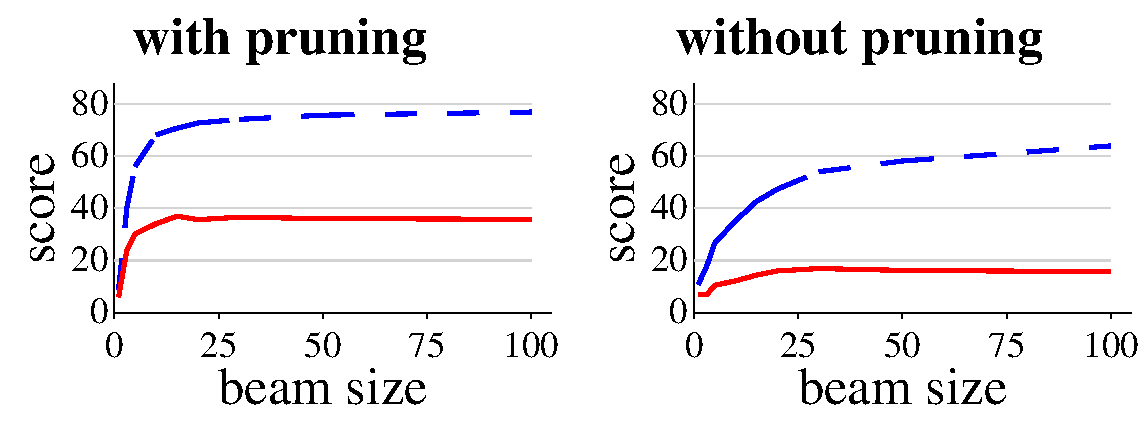
\includegraphics[scale=0.5]{sfig/sempre.slides/newBeamPlot.pdf}
\caption{
Accuracy (solid red) and oracle (dashed blue) scores with different beam sizes.
}
\label{fig:sempre-beam}
\end{figure}

\paragraph{Effect of beam size.}
Figure~\ref{fig:sempre-beam}
shows the accuracy and oracle scores
as the beam size changes.
A lower beam size increases efficiency
and prevents bad logical forms from clogging up the beam,
but when the beam size gets too low,
the accuracy and oracle scores decrease.

\subsection{Additional dataset analysis}
\label{sec:wtq-analysis-again}

Using the trained parser,
we continue our investigation from
Section~\ref{sec:wtq-analysis}
and empirically analyze several aspects of the
\wtq dataset.
% From Table~\ref{tab:sempre-results},
% our parser successfully finds a logical form
% consistent with the correct denotations in
% 76.7\% of the development examples.
% We use these consistent logical forms
% to examine the complexity of our dataset.

\paragraph{Logical form coverage.}
The \wtq dataset contains various types of reasoning
to answer the questions.
Table~\ref{tab:sempre-ablation}(c) shows the drop in accuracy
and oracle scores
when only a subset of deduction rules are allowed.
The \emph{join only} subset corresponds to table lookup,
while the \emph{join + count} subset covers the same scope
of logical forms as the previous work on the \Sc{WebQuestions} dataset
\cite{berant2013freebase}.
Finally, the \emph{join + count + superlative} subset
roughly corresponds to the coverage of the \Sc{GeoQuery} dataset \cite{zelle96geoquery}.

\begin{figure}[t]
\centering
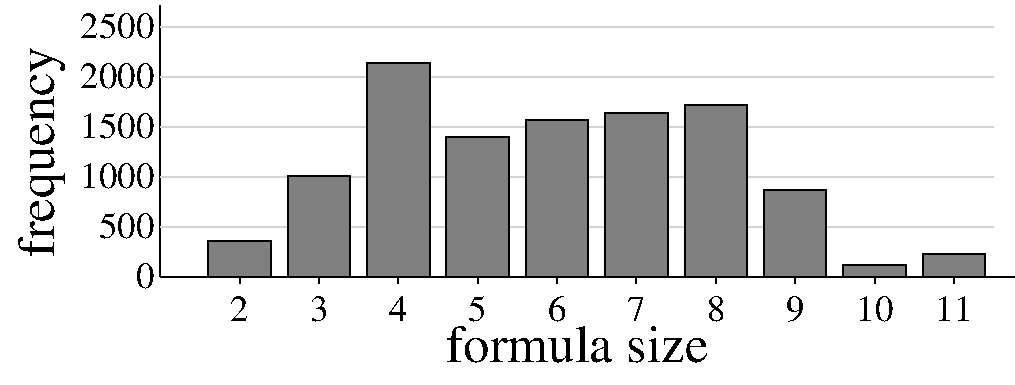
\includegraphics[scale=0.45]{sfig/sempre.slides/predCountHistogram.pdf}
\caption{
Sizes of the highest-scoring correct candidate logical forms in development examples.
}
\label{fig:sempre-lf-size}
\end{figure}

\paragraph{Compositionality.}
The histogram in Figure~\ref{fig:sempre-lf-size}
tracks the size of the logical forms
(as the number of compositional deduction rules)
that are consistent with the correct answer.
If there are consistent multiple logical forms in
the candidate set $\zx$, we choose the shortest one.
The histogram shows that a significant number of logical forms
have non-trivial sizes.

\subsection{True oracle score}
\label{sec:sempre-true-oracle}

From Table~\ref{tab:sempre-results},
our parser successfully generates a logical form
consistent with the correct denotations 
(but may or may not be the highest-scoring logical form)
in 76.7\% of the development examples.
Based on
the large gap between the accuracy (37.0\%) and this number,
one might believe that the accuracy can be improved
mainly with a better scoring model.
Unfortunately, the oracle score is misleading
due to the existence of \emph{spurious logical forms}
that give the right answer for wrong reasons.
For instance, in our running example (Figure~\ref{fig:sempre-running-ex}),
consider the spurious logical form
\begin{equation}
\xOf{Venue}.\T{argmax}(\xHas{Position}.\T{1st},
\lambda r[\xOf{Num}.\xOf{Time}.r]).
\end{equation}
From $\deno{\xHas{Position}.\T{1st}}{w} = \{r_2, r_4\}$,
the logical form picks the row with the highest \emph{Time}
instead of the highest index,
but eventually arrives at the 
correct denotation $\{\T{Thailand}\}$.
We found that in many examples,
the parser only found spurious logical forms
and not a semantically correct one.

To measure the true oracle score,
we sample 300 examples and manually annotate them
with semantically correct logical forms,
and see if the trained system can generate
the annotated logical form as a candidate.\footnote{
This method ignores generated logical forms
that are semantically
equivalent to the annotated logical forms.
Chapter~\ref{chp:dpd} will present
a more precise method that takes
logical form equivalency into account.
}
Out of 300 examples,
we find that 84\% can be manually annotated,
while the rest are unhandled questions
as explained in Section~\ref{sec:sempre-error-analysis}.

The system successfully generates the annotated
logical forms in only 53.5\% of the examples.
This indicates that the main method to improve the parser
is to increase the \emph{coverage} over answerable questions,
such as by augmenting the knowledge graph
and expanding deduction rules.
We will explore this direction of increasing coverage,
along with the efficiency problem it entails,
in the next chapter.

\section{Related work and discussion}

\paragraph{Logical form generation.}
Apart from the bottom-up generation used in our floating parser,
previous work has modelled the process of generating logical forms
with various paradigms.

Like the logical form structure,
the syntactic parse of a sentence is also hierarchical.
As such, previous work has considered using
syntactic structures to guide
the generation of semantic parses.
For instance, some take the syntactic parse
from an external parser and convert it into a semantic parse
\cite{poon2013gusp,reddy2016transforming}.
Others learn a joint model for syntactic and semantic parses.
One popular example is the use of
Combinatory Categorial Grammar
\cite{steedman1996surface,steedman00ccg}, or CCG,
which can capture syntax and semantics jointly
\cite{zettlemoyer05ccg,zettlemoyer07relaxed,kwiatkowski10ccg,kwiatkowski11lex}.

Without using syntactic structures,
one can also learn to decode the semantic parse directly.
We follow the line of work that uses
bottom-up generation
\cite{berant2013freebase,berant2014paraphrasing,berant2015agenda}.
One benefit of bottom-up generation is that
the intermediate parses are complete logical forms
that can be executed,
and the resulting denotations
can be used to prune unpromising logical forms
\cite{wang2018robust}
or as additional information
to the scoring model
\cite{guu2017bridging}.

Early \emph{neural} semantic parsing approaches
treat logical form generation as a sequence prediction problem
and just generate the predicates from left to right
\cite{jia2016recombination}.
This works well for generating canned idiomatic expressions,
but the resulting sequences are not guaranteed to be valid logical forms.
A popular alternative is top-down generation,
where at each recursion step,
the parser first selects an operator
and then recursively builds the arguments as child subtrees
\cite{dong2016logical,krishnamurthy2017neural,rabinovich2017abstract,cheng2017learning}.
One benefit of the top-down approach is that the information
from the parent node is properly propagated
to the corresponding children subtrees,
even when the subtree is generated many steps after the parent operator
is generated.

\paragraph{Hard mapping versus soft mapping.}

Early semantic parsing work assumes a strict mapping
between words in the utterance and predicates
in the logical forms.
This mapping is often called a \emph{lexicon},
which could be hand-specified
\cite{zelle96geoquery,unger2011pythia,unger2012template},
learned separately from the data
\cite{cai2013large,berant2013freebase},
or learned jointly while training the parser
\cite{zettlemoyer07relaxed,kwiatkowski10ccg,kwiatkowski11lex}.
While this works well for a specific domain,
learning such a lexicon for open-domain knowledge sources
is difficult due to the open set of phrases and predicates.
Previous work addressed this using factorized lexicon
\cite{kwiatkowski11lex}
or by translating the lexicon output to match the target
domain on the fly
\cite{kwiatkowski2013scaling}.

Our floating parser takes a similar approach to
the free-form generation of logical forms
in \citet{berant2014paraphrasing}.
Instead of a strict mapping,
we try out different logical form predicates and
uses the scorer to rank them.
This idea of soft mapping
has become the norm in neural-based parsers
\cite{jia2016recombination,dong2016logical,krishnamurthy2017neural},
where the generation of each predicate
is guided by the
embedding of the input,
while the attention mechanism \cite{bahdanau2015neural,luong2015translation}
is used as a soft alignment
between certain utterance tokens
and the generated logical predicate.
Open-domain predicates
(e.g., column and cell nodes in our case)
are generated using explicit copy mechanism
\cite{gu2016copying,jia2016recombination},
which plays a similar role to our terminal rules.

\paragraph{Table normalization.}
One challenge with working on web tables is that
the table format is not standardized.
This is surprisingly severe on Wikipedia:
while there are some general guidelines,
Wikipedia editors end up using
the most suitable table format for each article.

One way to handle the different table formats
is to convert them into canonical formats.
For instance, different table formatting can be canonicalized
to database-like formats
\cite{embley2016converting}.
Entities in the table can be linked to canonical entities
in some structured knowledge source
\cite{limaye2010annotating,bhagavatula2015tabel}.
Numerical cells can be parsed into the correct
values and units
\cite{madaan2016numerical}.
And missing data can be inferred
from an aggregation of multiple tables
\cite{venetis2011recovering}.
The canonicalization makes it easier
to perform computation on the data,
but it requires designing a good canonical schema.
Moreover, the conversion process is noisy
and might introduce errors for ambiguous cell contents.
For instance, the string
\nl{1990} is usually tagged as a date by a
named entity recognition (NER) tagger,
but could be a plain number
or a proper noun in some contexts.

Another way to handle tables
is to extract just the necessary information from the table
\cite{govindaraju2013understanding,zhang2015deepdive}.
The extracted information,
usually a relation between two entities,
can then be used to populate a database
with a known schema
\cite{ellis2015tackbp}.
Apart from having clean data suitable for computation,
this type of extraction also
allows the information from both structured data
and unstructured text to be unified and reasoned on jointly.
However,
it precludes the use of other data
available in the table that were not extracted.

Our approach is to maintain uncertainty in
table interpretation via normalization edges,
and then let the scorer
choose the correct
% The scorer is then responsible for choosing the correct
form of normalization.
This process prevents the loss of information
due to extraction.
Moreover, additional ways to interpret the cells
can be added dynamically,
as we will explore in Chapters~\ref{chp:macro}~and~\ref{chp:dpd}.
However, this also increase the search space of logical forms,
which is sometimes wasteful when the column
is clearly of a particular type.
For instance, the cell with text \emph{1990} is very likely to be a year
if all other cells also look like a year,
and keeping around the possible \T{Num} interpretation
wastefully expands the space of possible logical forms.

\section{Conclusion}
In this chapter,
we presented a semantic parsing approach for
the task of answering complex question on web tables.
To handle open-domain tables with unknown schemata,
we (1) use knowledge graph as a domain-generic representation
of the tables,
and (2) use a floating parser that can flexibly
generate logical form predicates based on the table schema.
The scoring function is then responsible for
relating the question to the generated logical forms.

To train the model with the correct answers as distant supervision,
we need to generate a set of candidate logical forms
and up-weight the ones that are consistent with the annotated answers.
Unfortunately, with more complex questions,
the space of possible logical forms rapidly expands
with the number of reasoning steps and logical operators.
This makes it expensive to generate a set of candidates
that contain a consistent logical form.
In the next two chapters, we will look at techniques
to control the search space of logical forms.


\chapter{Guiding Search with Logical Form Patterns}
\label{chp:macro}
\begin{table}[t]\centering\small
\begin{tabular}{@{\;}r@{ $\to$ }lll@{}} \toprule
\multicolumn{2}{c}{\textbf{Rule}} & \textbf{Semantics}
& \textbf{Example} \\ \midrule

$\C{TokenSpan}$ & $\C{Entity}$
& $\mathrm{fuzzymatch}(s)$
& $\T{China}$ \quad (from \nl{Chinese}) \\
\explainBLong{$\Mr{fuzzymatch(s)}$ generates cell nodes with string approximately matching $s$} \\

$\C{Values} + \C{ValueFn}$ & $\C{Values}$
& $S(z_1, z_2)$
& $\T{argmax}(\xOf{Event}.\T{allRows}, \lambda v[\T{count}(\xHas{Event}.v)])$ \\
\explainBLong{A \C{ValueFn}, as defined in Table~\ref{tab:sempre-compositional-rules},
maps cells or atomic values
into comparable values} \\

\bottomrule

\end{tabular}
\caption[Additional deduction rules to increase question coverage.]{
Additional deduction rules to increase the coverage
on answerable questions.
}\label{tab:macro-new-rules}
\end{table}

\begin{table}[t]
\centering
\begin{tabular}{ll} \toprule
\nl{Which driver appears the most?}
& $\T{argmax}(\xOf{Driver}.\T{allRows},
\lambda v[\T{count}(\xHas{Driver}.v)])$ \\
\nl{Is English for French spoken more?}
& $\T{argmax}(\T{English} \sqcup \T{French},
\lambda v[\T{count}(\xHas{Language}.v)])$ \\
\nl{Who is taller, Rose or Time?}
& $\T{argmax}(\T{Rose} \sqcup \T{Tim},
\lambda v[\xOf{Num}.\xOf{Height}.\xHas{Name}.v])$ \\
\bottomrule
\end{tabular}
\caption{Examples of superlative logical forms applied on sets of cell nodes.}
\label{tab:macro-superlative}
\end{table}

As mentioned at the end of the previous chapter (Section~\ref{sec:sempre-true-oracle}),
we would like to increase the coverage over
answerable questions by expanding the space
of logical forms that can be generated.
One way to achieve this is by expanding the
set of deduction rules.
In particular, we add new rules listed in
Table~\ref{tab:macro-new-rules},
which allows cells nodes to be generated
from approximate string matching
(e.g., the phrase \nl{Chinese} can now map to \T{China}),
and introduces superlatives on sets of cell nodes
as demonstrated in Table~\ref{tab:macro-superlative}.

Adding just these two rules
already increases the true oracle number
from 53.5\% %to \qqq\%.
by almost 10\% absolute.
This is because both rules directly address
the major coverage errors as analyzed in
Section~\ref{sec:sempre-error-analysis}.
However, since the added rules can potentially generate
many more candidate logical forms
(e.g., there can be multiple cells approximately
matching each utterance token span),
the increased coverage comes with a cost of
slower running time.
On average per example,
the training time increases from 619 ms to 1,117 ms,
and the prediction time increases from 645 ms to 1,150 ms.
This doubling of running time could mean additional days
to train and tune a model.
Even worse, the running time will increase even more
when the space of logical form is expanded further
to gain more question coverage.

%\section{Using patterns to guide search}

\begin{figure}[t]
\centering
\textsf{
\begin{tabular}{|c|c|c|c|c|} \hline
\textbf{Year} & \textbf{Venue} & \textbf{Position} & \textbf{Event} & \textbf{Time} \\ \hline
2001 & Hungary & 2nd & 400m & 47.12 \\
2003 & Finland & 1st & 400m & 46.69 \\
2005 & Germany & 11th & 400m & 46.62 \\
2007 & Thailand & 1st & relay & 182.05 \\
2008 & China & 7th & relay & 180.32 \\ \hline
\end{tabular}
}
\\[0.5em]
\begin{tabular}{r@{ }l}
$x=$ & \nl{Which location comes after Germany?} \\
$z=$ & $\xOf{Venue}.\xOf{Next}.\xHas{Venue}.\T{Germany}$ \\
$y=$ & \{\T{Thailand}\}
\end{tabular}
\caption{Our running example from before but with a different question.}
\label{fig:running-ex-macro}
\end{figure}

% As emphasized earlier,
% the need to handle open-domain web tables (\Breadth)
% and more complex questions (\Depth)
% causes the space of logical forms to explode quickly.
% In the previous chapter, we introduced methods
% to sidestep the issue
% by treating search as a preprocessing step.
% This chapter explores a different solution:
% following the original training method
% in Chapter~\ref{chp:parsing},
% we perform search during training,
% but we search more cleverly
% by using patterns of logical forms found in
% previously processed example to guide the search process.
% Our approach is based on two key ideas:

In this chapter,
we propose to speed up the parser
by making the search algorithm prioritize
logical forms that ``look good''
according to its past experience.
Our approach is based on two key ideas:

\begin{itemize}
\item
\textbf{Good logical forms share common patterns.}
%To give an intuition,
For example,
consider the question
\nl{Which location comes after Germany?}
for the table in Figure~\ref{fig:running-ex-macro}.
One possible semantically correct logical form is
\begin{equation}
\xOf{Venue}.\xOf{Next}.\xHas{Venue}.\T{Germany},
\end{equation}
%which executes to the correct answer \T{Thailand}.
which identifies the cell below \emph{Germany}
in the same \emph{Venue} column.
From this logical form,
we can abstract out question-specific and
table-specific predicates
(i.e., columns, cells, and primitive values) to get
the following \emph{macro}:
\begin{equation}
\aOf{\C{Col}\#1}.\xOf{Next}.\aHas{\C{Col}\#1}.\A{\C{Cell}\#2},
\end{equation}
which identifies the cell below $\A{\C{Cell}\#2}$
in the same $\A{\C{Col}\#1}$ column.
Such a macro captures a domain-independent
computational pattern
that generalizes across different table contexts.
The main idea of
our training procedure
is to extract macros
from logical forms found from search,
and then use them to efficiently construct
logical forms in new contexts.

\item
\textbf{Similar utterances are likely to share a
logical form pattern.}
Though the space defined by macros is smaller
than the original search space,
the set of extracted macros will eventually grow
with the number of processed examples.
To prioritize macros that are more likely to match
for the input question $x$,
we propose \emph{holistic triggering}:
find the $K$ examples with questions most similar to $x$,
and then only test macros extracted from
the consistent logical forms found in those examples.
\end{itemize}

Based on the two ideas above,
we propose an online learning algorithm
that jointly learns a semantic parser
and a set of macros
encoded as \emph{macro deduction rules}.
For each training example,
the algorithm first tries to find consistent logical forms
by using holistic triggering to invoke a subset
of promising macro rules to apply.
If it succeeds, the logical forms
are used to update the parameters of the semantic parser.
Otherwise, it falls back to the
base deduction rules to perform a more exhaustive search,
and then uses the discovered consistent logical forms
to derive more macro deduction rules.
At test time, we only use the learned macro deduction rules.

The next two sections describe the details of
macro deduction rules and the training algorithm.
Afterward, we evaluate our approach on the \wtq dataset
in terms of accuracy and speed.
Training with macro rules yields a 11x speedup
compared to training with the base deduction rules,
and at test time,
we achieve a slightly better accuracy of 43.7\%
with a 16x speedup compared to the baseline.

\paragraph{Reference.}
The results described in this chapter have been published as
\citet{zhang2017macro}.
Reproducible experiments are hosted on the
CodaLab platform at
\begin{center}
\small
\url{https://worksheets.codalab.org/worksheets/0x4d6dbfc5ec7f44a6a4da4ca2a9334d6e}.
\end{center}

\section{Macros}

\subsection{Deriving macros from logical forms}

\begin{figure}
\centering
\begin{subfigure}[b]{\textwidth}\centering
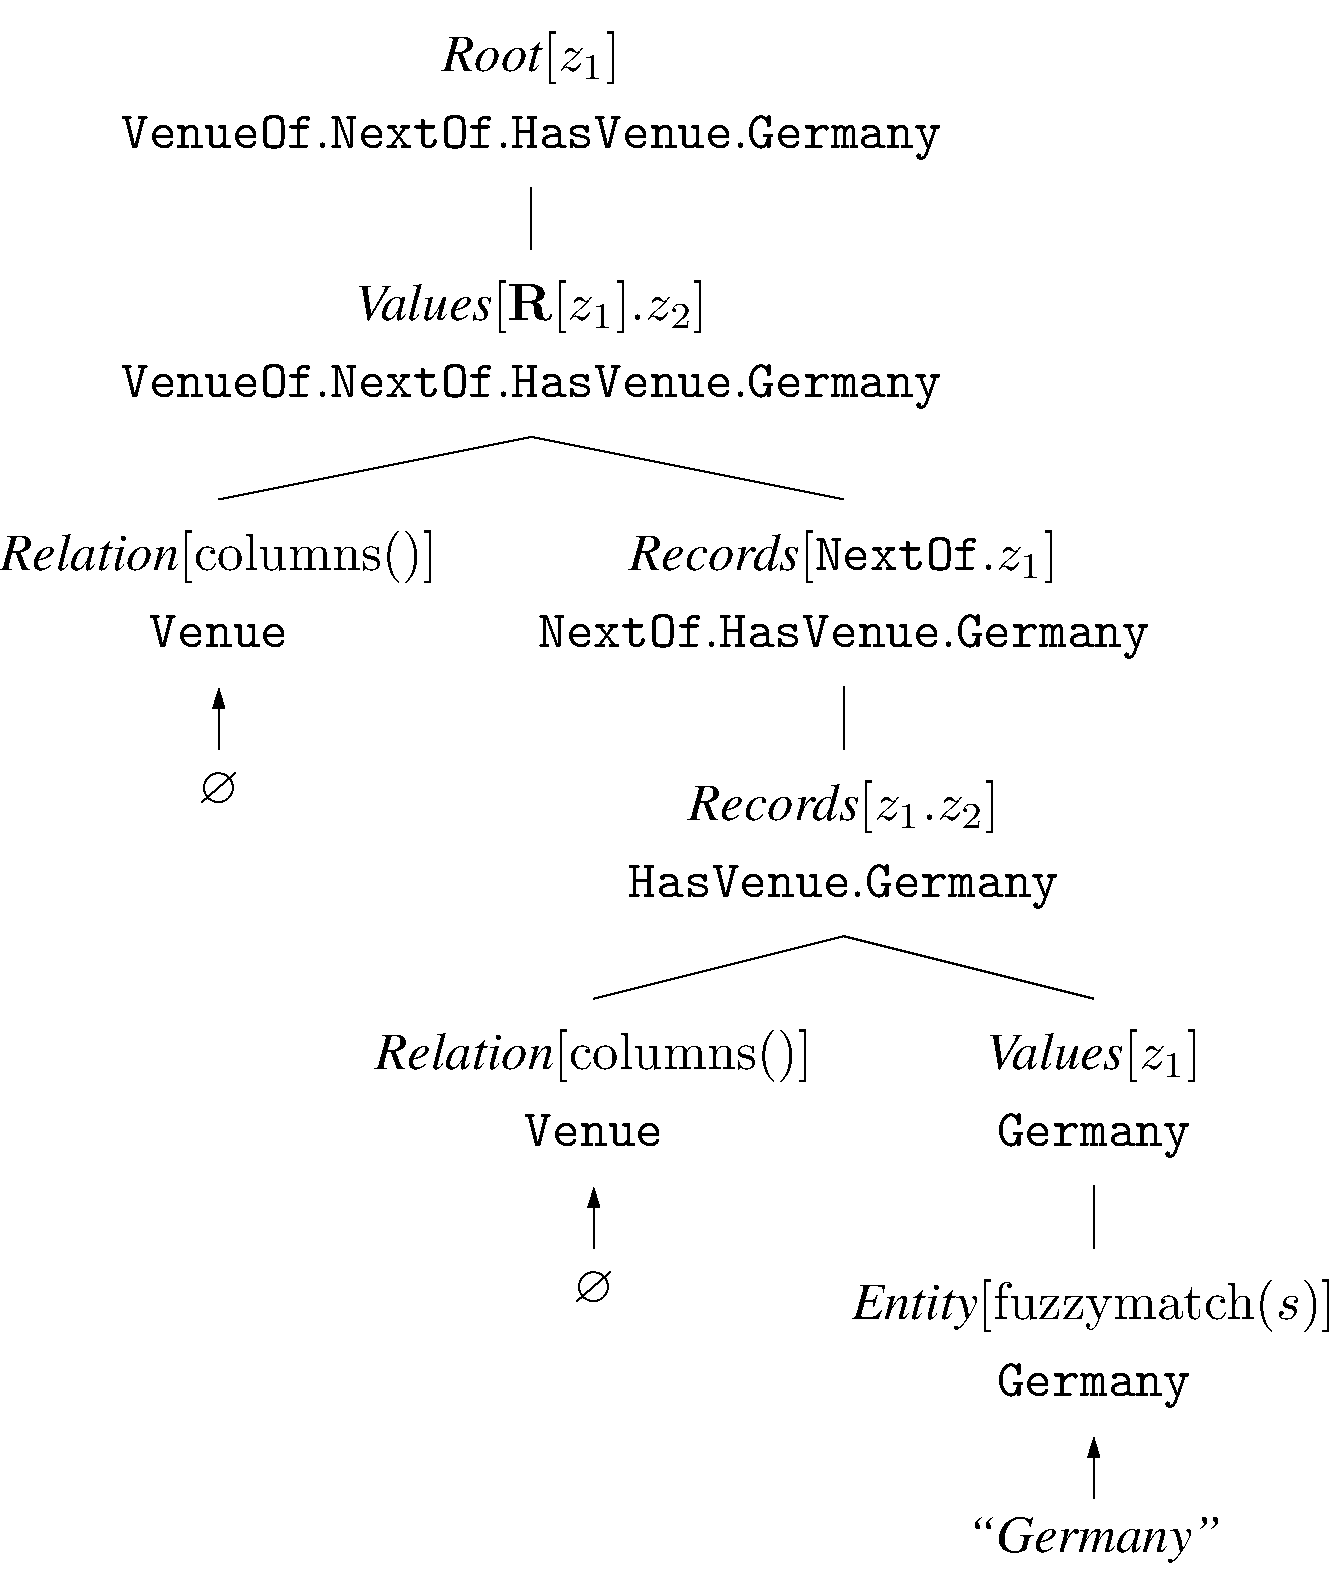
\includegraphics[scale=.35]{sfig/parsetrees.slides/macroParseOrig.pdf}
\caption{Derivation tree ($z_i$ represents the $i$th child)}
\label{fig:compute-macro-a}
\end{subfigure} \\[1em]
\begin{subfigure}[b]{0.40\textwidth}\centering
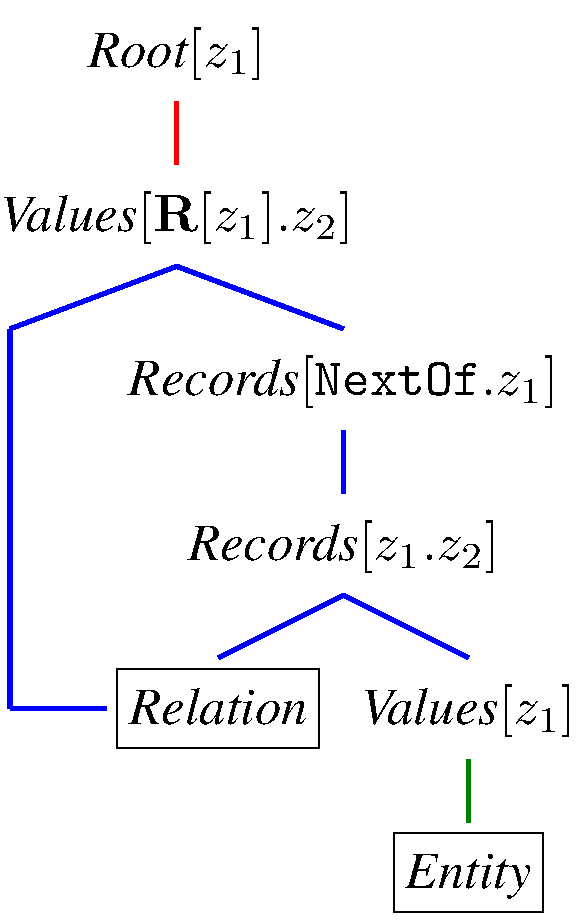
\includegraphics[scale=.35]{sfig/parsetrees.slides/macroParseMacro.pdf}
\caption{Macro}
\label{fig:compute-macro-b}
\end{subfigure}
\begin{subfigure}[b]{0.40\textwidth}\centering
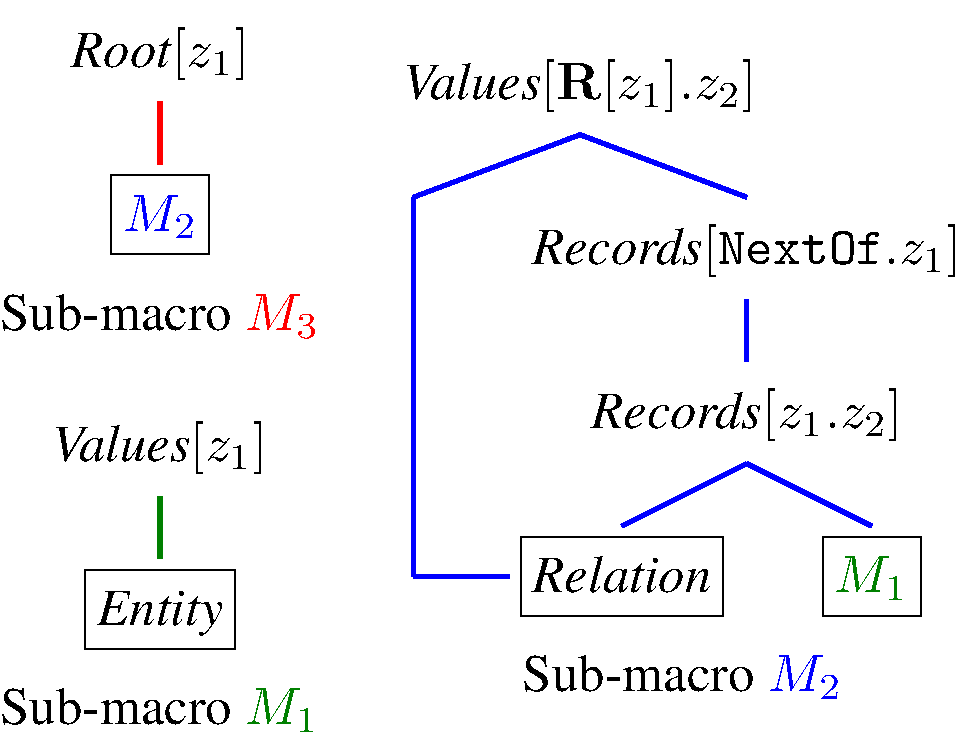
\includegraphics[scale=.35]{sfig/parsetrees.slides/macroParseSubMacros.pdf}
\caption{Atomic sub-macros}
\label{fig:compute-macro-c}
\end{subfigure}
\caption[
Derivation of macro deduction rules.
]{From the derivation tree (a), we extract a
macro (b), which can be further decomposed into
atomic sub-macros (c). Each sub-macro is converted
into a macro rule.}
\label{fig:compute-macro}
\end{figure}

A \emph{macro} $M$
characterizes an abstract logical form structure.
For any given logical form $z$,
we can compute its macro by transforming its derivation tree
as illustrated in Figure~\ref{fig:compute-macro}:
\begin{enumerate}
\item
For each terminal deduction rule (i.e., leaf node),
substitute it with a placeholder,
and label it with the category of that derivation
(i.e., the category on the right hand side of the
deduction rule).
\item
Merge leaf nodes that represent the same
partial logical forms.
For instance, the two mentions of \T{Nation}
in Figure~\ref{fig:compute-macro-b}
are merged to signify that the two column names
have to be identical.
\end{enumerate}

The resulting macro $M$ can be serialized as a flat string
by assigning an index to each placeholder
as illustrated in the figure.
While the resulting macro is not a tree,
we will use the terms \emph{root} and \emph{leaf}
to refer to nodes that were roots or leaves
in the original derivation tree.

A logical form $z'$ satisfies the macro
if it can be obtained by filling each placeholder in $M$
with a value of the matching category.
For instance,
the logical form
$z' = \xOf{Year}.\xOf{Next}.\xHas{Year}.\T{1st}$
satisfies the macro $M$ in the figure
(even though it executes to an empty set).

\subsection{Macro deduction rules}
For any macro $M$, we can construct a set of
\emph{macro deduction rules} that,
when combined with terminal rule from the 
original set of deduction rules
(called ``base deduction rules'' henceforth),
generates exactly the logical forms that satisfy
the macro $M$.
The most basic approach is to construct a single rule
for the whole macro:
if the placeholders of $M$ are labeled $c_1, \dots, c_k$,
we construct a deduction rule
\begin{equation}
c_1[z_1] + \dots + c_k[z_k] \to
\C{Root}[f(z_1, \dots, z_k)]
\end{equation}
where $f(z_1, \dots, z_k)$
is a semantic function that substitute $z_1, \dots, z_k$
to the corresponding placeholder nodes of $M$.
For example, the macro in Figure~\ref{fig:compute-macro-b}
yields a deduction rule
\begin{equation}
\C{Relation}[z_1] + \C{Entity}[z_2] \to
\C{Root}[\Mb{R}[z_1].\xOf{Next}.z_1.z_2]
\end{equation}

\paragraph{Decomposed macro deduction rules.}
To speed up the model,
we want to avoid processing the same
logical form fragment more than once.
For instance,
when we use macro deduction rules to generate
\begin{equation}
\T{max}(\xOf{Num}.\xOf{Year}.\xHas{Position}.\xHas{Num}.\C{1})
\end{equation}
and
\begin{equation}
\xOf{Venue}.\T{argmin}(\xHas{Position}.\xHas{Num}.\C{1},
\lambda r.\xOf{Index}.r),
\end{equation}
we want to avoid constructing and featurizing
the same fragment $\xHas{Position}.\xHas{Num}.\C{1}$
multiple times.
%
To achieve this goal,
we decompose macros $M$ into \emph{sub-macros}
and define deduction rules from them.
A subgraph $M'$ of $M$ is a sub-macro of $M$ if
\begin{enumerate}
\item $M'$ contains at least one non-leaf node
\item $M'$ connects to the rest of the graph ($M\setminus M'$)
only through the root of $M'$.
\end{enumerate}
A macro $M$ is \emph{atomic} if its only sub-macro is itself.
The process of decomposing a non-atomic macro $M$,
as illustrated in Figure~\ref{fig:compute-macro-c},
is as follows:
\begin{enumerate}
\item 
Detach an atomic sub-macro $M'$ from $M$
and define a macro rule
\begin{equation}
c'_1[z_1] + \dots + c'_k[z_k] \to c'_\Mr{out}[f(z_1, \dots, z_k)]
\end{equation}
where $c'_1, \dots, c'_k$
are the categories of the leaf nodes of $M'$,
and $f(z_1, \dots, z_k)$ is a semantic function
that substitutes $z_1, \dots, z_k$ into the macro $M'$.
The name of the category $c'_\Mr{out}$
is computed by serializing $M'$ as a string;
this way, if the sub-macro $M'$
appears in a different macro,
the category name will be shared,
and any logical form satisfying $M'$ will only be
constructed once.
\item
Substitute the subgraph $M'$ in $M$
by a placeholder node with name $c'_\Mr{out}$.
\item
Repeat Steps 1 and 2 on the new graph
until we are left with an atomic macro,
and define a final macro deduction rule for it.
\end{enumerate}

\section{Training algorithm}

\begin{algorithm}[t]\setstretch{1.1}
\caption{Process a training example with macro rules}
\label{alg:macro-algorithm}
\begin{algorithmic}[1]
\Require training example $(x, w, y)$, macro rules,
base rules with terminal rules $\Mc{T}$
\State Select a set $\Mc{R}$ of macro rules based on $x$ with holistic triggering
\State Generate a set $\zx$ of candidate logical forms
from rules $\Mc{R} \cup \Mc{T}$
\If {$\zx$ contains consistent logical forms}
\State Update model parameters
\Else
\State Apply the base rules to search for a consistent
logical forms
\State Augment the macro rules
\EndIf
\State Associate utterance $x$ with the highest-scoring
consistent logical form found
\end{algorithmic}
\end{algorithm}

We now describe an online algorithm
that jointly learns the semantic parser
and macro deduction rules.
Algorithm~\ref{alg:macro-algorithm}
describes how our algorithm proceeds
for each training example $(x, w, y)$.
It first tries to use a subset of macro deduction rules
to search for logical forms.
If the search succeeds,
then the semantic parser parameters are updated as usual.
Otherwise, it falls back to the base deduction rules,
and then add new macro rules based on the
consistent logical forms found.

\subsection{Holistic triggering}
\label{sec:macro-trigger}

The first step of our algorithm is to
select a subset $\Mc{R}$ of macro rules
that are likely to generate consistent logical forms
for the question $x$.
The selection is done as follows.
Throughout training,
we maintain a mapping $\Mc{S}$
from each previously processed question
to a consistent logical form found while processing that question.
(Questions for which
a consistent logical form has not been found
are not included.)
Given a new training question $x$,
we identify $K$ questions in $\Mc{S}$
that are the most ``similar'' to $x$
(i.e., $K$-nearest neighbors of $x$ under some similarity metric),
and then let $\Mc{R}$
be the set of macro deduction rules that
were extracted from their associated logical forms.

\paragraph{Question similarity metric.}
We use token-level Levenshtein distance as
the distance metric for computing the nearest neighbors.
To compute the distance between two sentences $x$ and $x'$,
we first preprocess them by lemmatizing the tokens,
and then removing all determiners and infrequent nouns
that appear in less than 2\% of the training questions.
The distance is then defined as the Levenshtein distance
between the two sequences of remaining tokens.
For instance, \nl{\textbf{Who} ranked \textbf{right after} Germany}
and \nl{\textbf{Who} took office \textbf{right after} Uriah Forrest}
have distance 4.
Despite its simplicity, our distance is good at
capturing structural similarity between questions.

To speed up training,
we pre-compute a sorted list of $K_\Mr{max} = 100$
nearest neighbors for every question in the training data.
When processing a question $x$ during training,
we calculate $\Mc{R}$ as
the intersection of the pre-computed list for $x$
and the set of questions in $\Mc{S}$.

\subsection{Updating the macro rules}
The computed subset $\Mc{R}$ of macro deduction rules
is combined with the set $\Mc{T}$ of base terminal rules
(for building basic units such as \C{Cell} and \C{Col}).
The floating parser parses the training question $x$
using deduction rules $\Mc{R} \cup \Mc{T}$,
resulting in a set $\zx$ of logical forms
(Line~2 of Algorithm~\ref{alg:macro-algorithm}).

If $\zx$ contains a consistent logical form,
we update the model parameters as usual
(Line~4);
otherwise, we fall back to performing
beam search using the base rules
(Line~6).
For efficiency, we stop the search
either when a consistent logical form is found,
or when the total number of generated logical forms
exceeds some threshold $T$.
These early stopping criteria prevent
the model from spending too much time on
difficult examples
(e.g., when the context table is large).
While we might miss consistent logical forms
and thus their macros on such examples,
we could potentially induce the same macro
from more straightforward examples.

When the algorithm succeeds at finding a consistent
logical form $z$ with the base rules,
we extract its macro $M$
and construct the corresponding decomposed macro rules
(Line~7).
Parameters of the parser are not updated
when the beam search with base rules is invoked.

Finally, if a consistent logical form $z$ is found,
the mapping $\Mc{S}$ is updated to map $x$ to $z$
(Line~8).

\subsection{Prediction}
At test time,
we follow steps 1--2
of Algorithm~\ref{alg:macro-algorithm}
to generate a set $\zx$ of candidate logical forms
from the triggered macro rules
and base terminal rules.
We then output the highest-scoring logical form $z \in \zx$.
We do not fall back to beam search at test time.

\section{Experiments}

We evaluate our approach on the \wtq dataset.
In addition to the test accuracy,
we will also compare the running times
during both training and test time.

\paragraph{Model details.}
We use the same features and logical form pruning strategies
from Chapter~\ref{chp:parsing}.
We use a beam size of $B = 100$ for beam search,
and use $K = 40$ for the $K$-nearest neighbor
in holistic triggering.
We take 3 passes over the training data during training.
When falling back to beam search,
we stop the search when the number of generated logical forms
reaches $T = 5000$ in the first pass.
To further increase speed,
we disallow falling back to beam search
during the subsequent passes
(which means that no more macro deduction rules
are constructed after the first pass).

\subsection{Main results}

\begin{table}[t]\centering
\begin{tabular}{lcc}\toprule
& \textbf{Dev} & \textbf{Test} \\ \midrule
Original deduction rules (Chapter~\ref{chp:parsing}) & 37.0\%	&37.1\%\\
% \citet{neelakantan2016neural}	&37.5\%&	37.7\%\\
% \citet{haug2017neural}	&-&	38.7\%\\\hline
New deduction rules	& \textbf{40.6\%}	&42.7\%\\
New deduction rules + macros & 40.4\%	& \textbf{43.7\%} \\
\bottomrule
\end{tabular}
\caption{Results of learning with macros on the \wtq dataset.
}\label{tab:macro-accuracy}
\end{table}

\newcommand{\midhead}[1]{\multicolumn{1}{c}{\textbf{#1}}}
\begin{table}[t]
\centering
\begin{tabular}{lrrr}
\toprule
& & \multicolumn{2}{c}{\textbf{Time (ms/ex)}} \\ \cmidrule{3-4}
& \midhead{Acc.} & \midhead{Train} & \midhead{Pred} \\
\midrule
Original deduction rules (Chapter~\ref{chp:parsing})
& 37.0\% & 619 & 645 \\
New deduction rules & \textbf{40.6\%} & 1,117 & 1,150 \\
New deduction rules + macros & 40.4\%  & \textbf{99} & \textbf{70} \\
\quad no holistic triggering & 40.1\% &  361 & 369 \\
\quad no macro decomposition & 40.3\% & 177 & 159 \\
\bottomrule
\end{tabular}
\caption[Running time of macro rules]
{Comparison and ablation study. The columns report averaged prediction accuracy, training time, and prediction time (milliseconds per example) on the three development splits.}\label{tab:macro-time}
\end{table}

\paragraph{Test accuracy.}
Table~\ref{tab:macro-accuracy} shows the test accuracy
of our approach and other parses on the \wtq dataset.
Compared to the original floating parser,
learning with macros slightly improves the test accuracy
from 42.7\% to 43.7\%,
while the averaged development accuracy on three development splits
are similar for the two approaches
(40.6\% vs 40.4\%).

\paragraph{Running time.}
Table~\ref{tab:macro-time} lists the
running time needed to process an example
in the original floating parser
and our new approach.
We trained all parsers on a machine
with Xeon 2.6GHz CPU and 128GB memory without parallelization.
Learning with macros is substantially
more efficient, with 11x speedup during training
and 16x speedup at test time.

\paragraph{Ablation analysis.}
We run two ablations of our algorithm:
removing holistic triggering
(i.e., consider all macro rules when parsing a question $x$)
and removing macro decomposition
(i.e., construct a single deduction rule for each macro).
Table~\ref{tab:macro-time}
shows that the ablated models are slower
to process examples.
This is because holistic triggering
greatly narrows down
the set of macro rules for parsing questions,
while decomposed macro rules
save us from featurizing the same
logical form fragments multiple times.

\subsection{Coverage of macros}
Using the base deduction rules,
the floating parser generates an average of 13,700
partial logical forms for each training example,
and discovers a consistent logical form
in 81.0\% of the examples.
When learning with macros,
the numbers become 1,300 and 75.6\%.

At a first glance,
learning with macros seems to
reduce the coverage of logical forms,
but this is untrue once we factor out spurious logical forms
(i.e., logical forms that execute to the right denotation
for wrong reasons).
% However, the discovered consistent logical forms
% also include spurious logical forms.
To measure the coverage over semantically correct logical forms,
we turn to the 300 examples that
we annotated with correct logical forms in Chapter~\ref{chp:dpd}.
We find that for 48.7\% of these examples,
the top consistent logical form produced
by the base deduction rules is semantically correct
(i.e., exactly matches
or is equivalent to the annotated logical form).
When learning with macros,
the number stays at 48.7\%,
meaning that the effective coverage
of the learned macro deduction rules
is as good as the base ones.


% \begin{table}\centering
% \input{figures/wtq/top-macros.tex}
% \caption{Top macros learned from the \wtq dataset and their semantics.}
% \label{tab:macros-top-macros}
% \end{table}

% \paragraph{Extracted macros.}
% Our approach extracts 123 macros in total.
% Among the training examples
% that the algorithm can find a consistent logical form,
% the top 34 macros listed in Table~\ref{tab:macros-top-macros} cover 90\%
% of those logical forms.

\subsection{Influence of hyperparameters}

\begin{figure}[t]
\begin{subfigure}[b]{0.333\textwidth}\centering
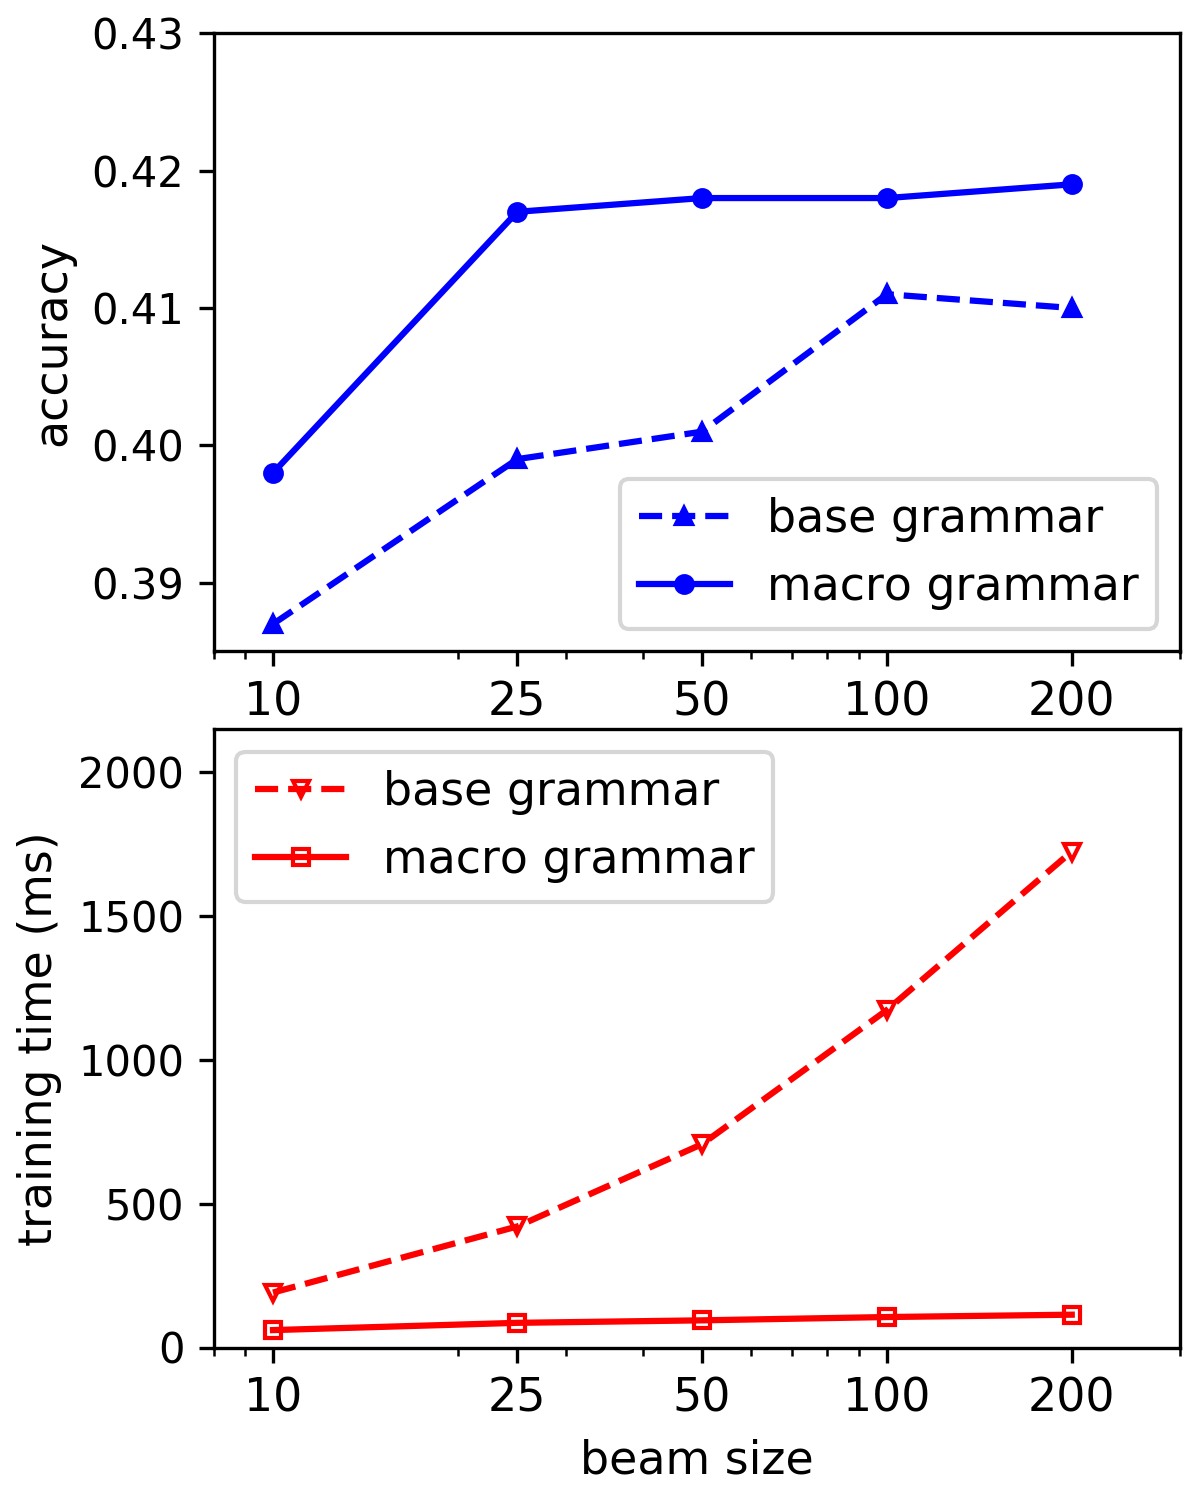
\includegraphics[width=1.0\linewidth]{figures/wtq/beamsize_split_high.png}
\caption{Varying beam size}
\label{fig:macro-hyperparam-a}
\end{subfigure}%
\begin{subfigure}[b]{0.333\textwidth}\centering
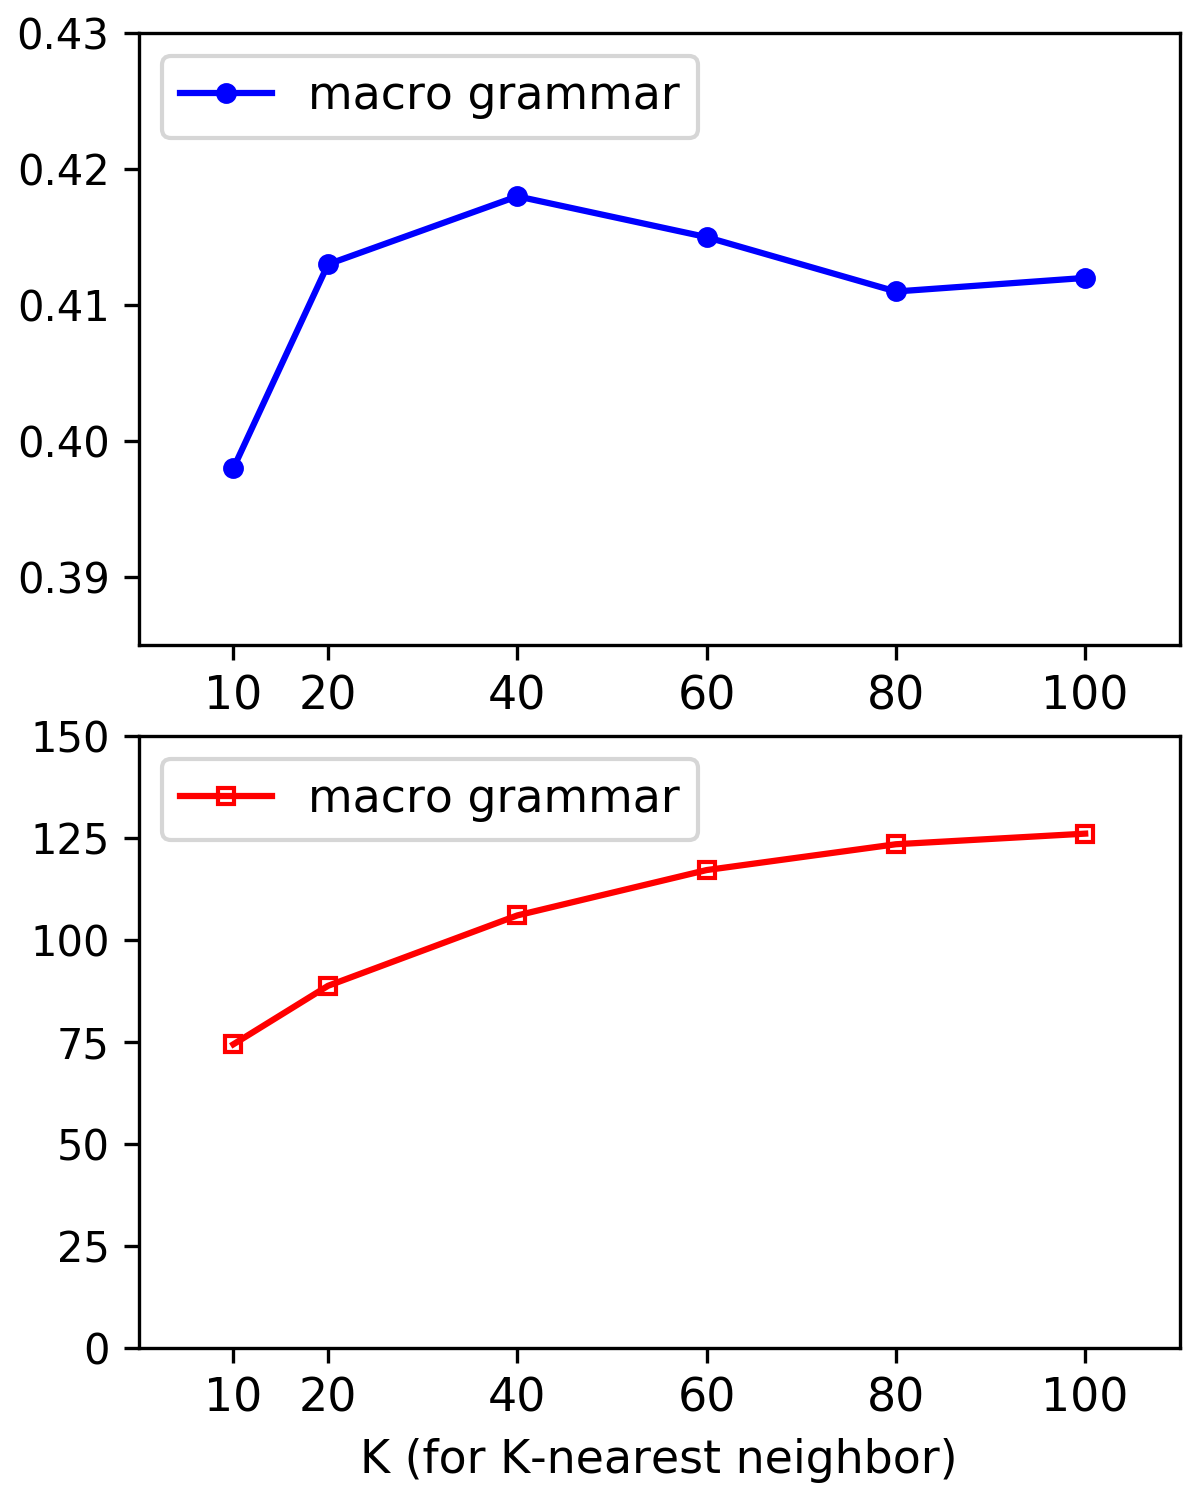
\includegraphics[width=1.0\linewidth]{figures/wtq/nn_k_split_high.png}
\caption{Varying neighbor size}
\label{fig:macro-hyperparam-b}
\end{subfigure}%
\begin{subfigure}[b]{0.333\textwidth}\centering
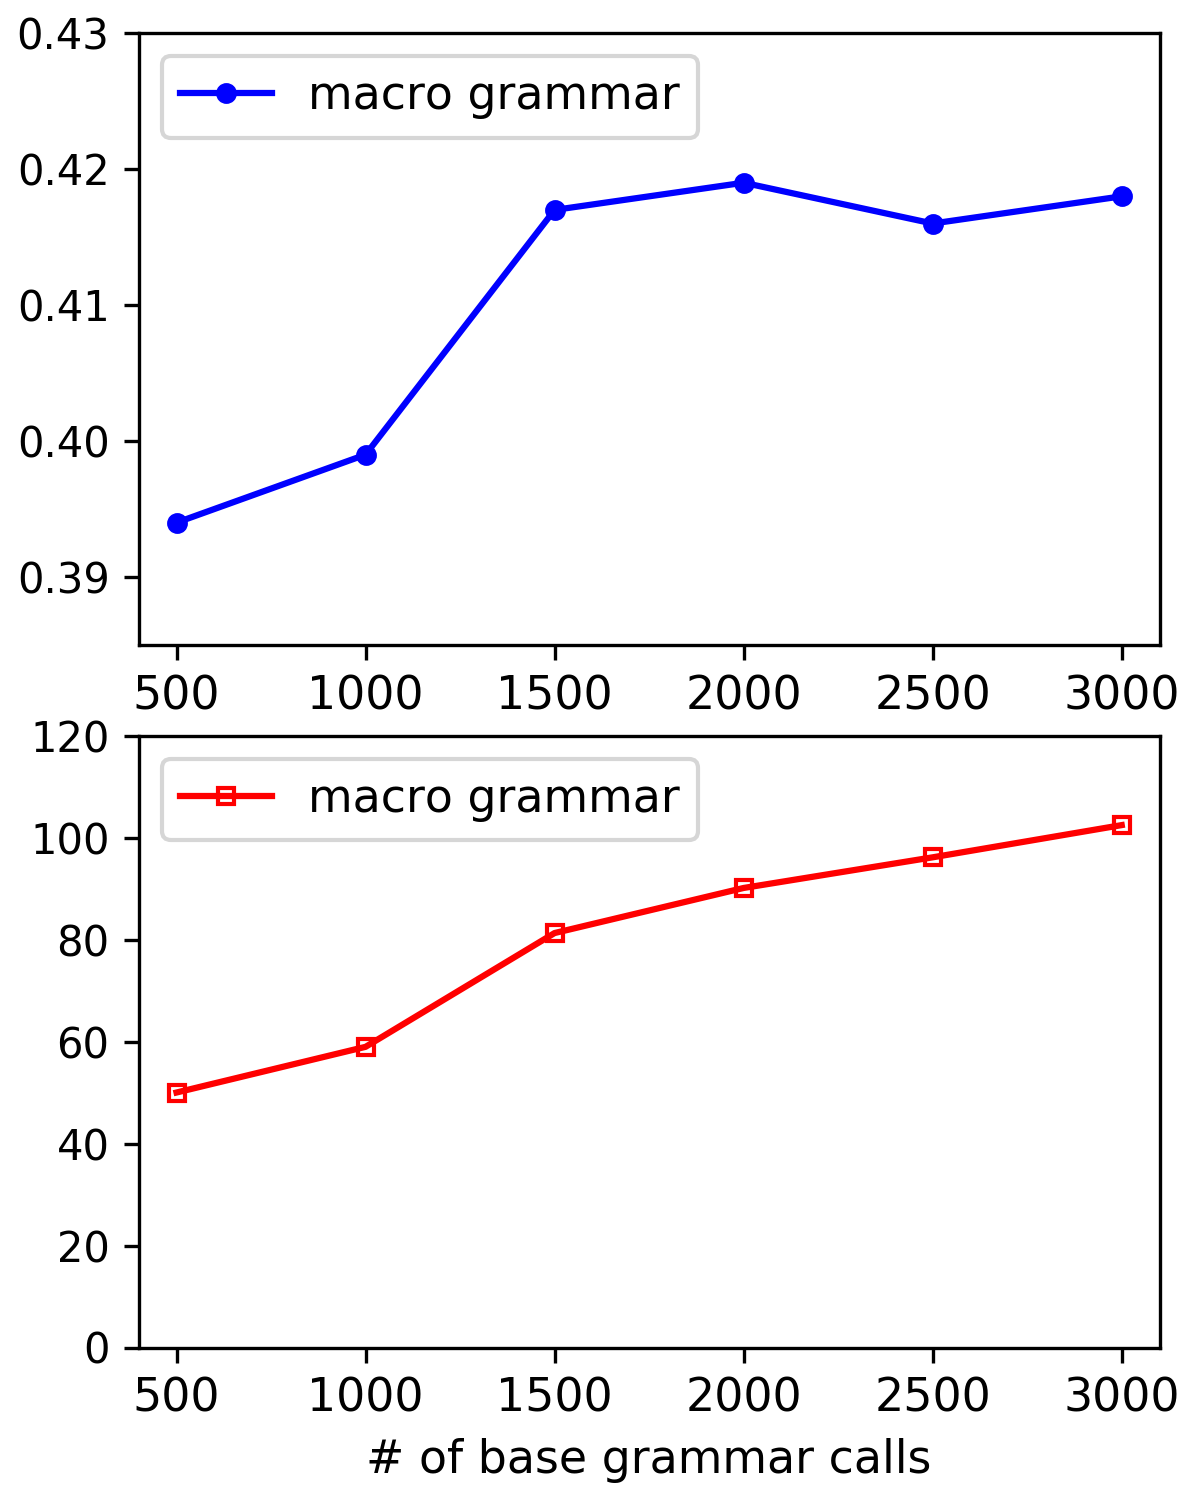
\includegraphics[width=1.0\linewidth]{figures/wtq/max_exploration_split_high.png}
\caption{Varying base rules usage count}
\label{fig:macro-hyperparam-c}
\end{subfigure}
\caption[Accuracy and training time with various hyperparameter choices]{
Accuracy and training time (per example) with various
hyperparameter choices, reported on the first train-dev split.
}\label{fig:macro-hyperparam}
\end{figure}

We compare the accuracy and training time per example
on the first development split of the dataset
when hyperparameters varies.

\paragraph{Beam size.}
Figure~\ref{fig:macro-hyperparam-a}
shows that for all beam sizes $B$,
training with macros is more efficient than
with the base deduction rules,
and the speedup rate grows with beam size.
The accuracy is robust to the varying beam size
as long as $B \geq 25$.

\paragraph{Number of neighbors in holistic triggering.}
We now consider $K$,
the number of neighboring questions
when computing the subset $\Mc{R}$ of macro rules
in Section~\ref{sec:macro-trigger}.
Figure~\ref{fig:macro-hyperparam-b}
shows that retrieving fewer similar questions
speeds up training but decreases accuracy.
On the other hand,
retrieving too many similar questions
can overload the list $\Mc{R}$
with potentially spurious macros,
which could explain why the accuracy
slightly drops when $K$ is too high.

\paragraph{Number of fallback searches.}
We perform ablation experiments
where we limit the number of times
that the algorithm can fall back to 
beam search on base deduction rules to at most $m$ times.
This effectively limits the number of macros
that the algorithm can discover:
the set of macro rules will be augmented 
at most $m$ times.
With smaller $m$, the accuracy grows with $m$,
which suggests that discovering a richer set of macros
improves the accuracy.

However, the accuracy changes much more slowly
once $m$ hits 1,500.
This suggests that we could speed up the model
even further by stopping the model from
finding macros after it has processed
some fraction of the training data.
Indeed, we try training a model with $B = 50$,
$K = 40$, and $m = 2000$.
The resulting model reduces the development accuracy
very slightly (down from 40.4\% to 40.2\%),
but it achieves more speed up during both training time
(up from 11x the base floating parser to 15x)
and test time
(up from 16x to 20x).

\section{Related work and discussion}

\paragraph{Modeling recurring structures.}
A few generative models have been proposed
to model recurring structures.
Examples of these models include adaptor grammars
\cite{johnson06adaptor}
and fragment grammars
\cite{odonnell11fragment},
which were designed to assign
higher probabilities to the structures
that use the reoccurring parts.
One example application of such models in semantic parsing
is the idiom-based program synthesis work by \citet{iyer2019learning},
where the common program idioms,
such as nested for-loops,
can be extracted from a large
library of unlabeled data.
The idioms are then added to the set of possible
production rules in a similar way to how
we add macro rules (without decomposition).
And like how our macro rules are used,
the idiom can be invoked during decoding
to produce a whole section for the desired program.

The main difference between our macro grammar
and these generative models
is that the generative models aim to improve modeling,
using the intuition that
learning to predict the repeating structure as a single action
is easier than learning to generate all parts.
% Since we only have distant supervision,
% our approach learns such idioms in an online fashion.
In contrast, our training algorithm
caches the patterns only to speed up search,
while the score assignment is done by a discriminative
scorer.
Nevertheless, we also notice a slight modeling improvement
on the test data.

\paragraph{Explicit mapping of phrases to logical form patterns.}
Previous semantic parsing work
has proposed a few methods to infer explicit
mappings from utterance phrases to logical form patterns.
For instance, the higher-order unification method
\cite{kwiatkowski10ccg,kwiatkowski11lex}
learns such a mapping in an online fashion
during training.
The result is a lexicon where each entry
contains a logical form template and a set of possible phrases
for triggering the template.

Our macros are triggered not by explicit mappings,
but instead use holistic triggering to
over-suggest the plausible macros to use.
This is similar to how the floating parser generates
some predicates independently from the utterance
with a soft guidance from the scorer.
This allows us to generate logical forms for utterances
containing unseen lexical paraphrases.
Moreover, our holistic triggering also works
when the triggers is not a local contiguous part
of the utterance.
For instance, the question
\nl{\textbf{Who is} older, Jack \textbf{or} John?}
can trigger the macro learned from
\nl{\textbf{Who is} taller, Rose \textbf{or} Tim?}:
the logical form pattern of applying \T{argmax}
on the union of two entities is dependent on the
whole structure of the sentence.

\paragraph{Sketch-based and retrieval-based program synthesis.}
The process of producing a logical form pattern
and filling in the details
is closely related to sketch-based program synthesis
\cite{solar05sketching}.
To generate a program,
the program sketch containing placeholders
is first chosen,
and then a synthesis algorithm
(search-based or solver-based)
is used to find the values for the placeholders
that make the program satisfy the program specification.
This technique has been
recently applied in the context of
neural semantic parsing
\cite{dong2018coarse},
where both the sketch and the actual logical forms
are generated using neural decoders:
the sketch is first generated based on the input,
then a second network encodes the sketch
and decodes the actual logical form.
When the target logical form is available,
the sketch can be directly inferred
and used to train the sketch generator.
In our case, we use the logical forms found by beam search
to create macros (cf.\ sketches),
and the macros in turn helps make search faster.

Another related approach is retrieval-based synthesis
\cite{gu2017search,hayati2018retrieval,guu2018edit}.
To generate an output for the current input $x$,
the output $y'$ of a similar input $x'$ in the corpus
is retrieved, and then the model uses $y'$
to generate an output $y$ for our input $x$.
Unlike our work which derives and caches macros,
these retrieval-based approaches can use the raw corpus
without having to preprocess it.

\section{Conclusion}
We have presented an algorithm to speed up both the
training and prediction time of our floating parser.
Under the assumption that logical forms
for similar utterances tend to share
the same pattern,
we use macro deduction rules to encode logical form patterns,
and use holistic triggering to choose the macro rules
that are the most relevant for the question.
Our approach can trade off between 
exploitation (applying macro deduction rules)
and exploration (falling back to beam search)
to achieve a large speed up without sacrificing the accuracy.
This allows us to efficiently expand the deduction rules
and knowledge graph representation so that more types of questions
can be answered.

One downside of our approach is that,
as a caching mechanism,
the macro rules do not kick in during the beginning of
the training process.
For the first few training examples,
not many macro rules have been accumulated,
which curtails the level of speed up seen in the final experiments.
Even worse, during early training iterations,
the parameters of the scoring function
are still not well-calibrated.
This leads to beam search pruning away
essential logical form parts,
and thus we are less likely to find a consistent logical form
when falling back to beam search.

% Since the distant supervision from annotated answers
% requires us to search over logical forms during training,
% we can get rid of search problems by
% changing the type of supervision.
% In the next chapter, we will explore techniques for converting
% the distant supervision (denotations) in the dataset
% to direct supervision (logical forms).
% While the conversion process also involves a search algorithm,
% additional information from the annotated answer
% and minimal crowdsourcing will allow us to
% overcome of the challenges when searching over the space
% of logical forms.


\chapter{Precomputing Semantically Correct Logical Forms}
\label{chp:dpd}
% In the previous chapter,
% we framed the task of answering a question $x$ on a table $w$
% as a semantic parsing task:
% generate a set $\zx$ of candidate logical forms,
% and then output $z \in \zx$ with the highest score.
% The goal is to predict a \emph{consistent} logical form;
% i.e., a logical form $z$ whose denotation
% matches the right answer $y$.

% While using patterns to guide search
% as explained in Chapter~\ref{chp:macro}
% increases the overall efficiency,
% performing search over the logical forms during training
% still poses two other fundamental issues.

So far,
we have been using the correct denotation (annotated answers)
as a distant supervision for training the semantic parser.
As argued in Chapter~\ref{chp:tables},
using distant supervision has several benefits.
Since the annotators do not have to learn the syntax of logical forms,
more annotations can be gathered more cheaply.
Furthermore, the annotation is independent of logical formalism,
meaning that we are free to choose any logical formalism
to attack the task.
Finally, more diverse types of questions can be gathered
since we do not limit the types of logical operations that
can be performed.

Despite these benefits,
training with denotation as supervision
requires running a search algorithm to find consistent logical forms
for parameter updates.
While doing so is fine in closed-domain settings,
% During training,
% the parser spends its time searching for logical forms
% by constructing them with deduction rules.
with the increased domain size (\Breadth)
and question complexity (\Depth),
it is increasingly
difficult to search over the space of logical forms
for two reasons:

\begin{figure}[tp]
\centering
\textsf{
\begin{tabular}{|c|c|c|c|c|} \hline
\textbf{Year} & \textbf{Venue} & \textbf{Position} & \textbf{Event} & \textbf{Time} \\ \hline
2001 & Hungary & 2nd & 400m & 47.12 \\
2003 & Finland & 1st & 400m & 46.69 \\
2005 & Germany & 11th & 400m & 46.62 \\
2007 & Thailand & 1st & relay & 182.05 \\
2008 & China & 7th & relay & 180.32 \\ \hline
\end{tabular}
}
\begin{tabular}{r@{\; }l}
$x$: & \nl{Where did the last 1st place finish occur?} \\
$y$: & Thailand \\
\end{tabular}
\\[0.5em]
%
\begin{tabular}{r@{\; }l} \toprule
\addlinespace

\multicolumn{2}{c}{\textbf{Consistent and semantically correct}} \\
\addlinespace

$z_1$: & {$\xOf{Venue}.\T{argmax}(\xHas{Position}.\T{1st}, \lambda r[\xOf{Index}.r])$} \\
\explainD{Among the rows with \emph{Position} = 1st, pick the one with maximum index and return its \emph{Venue}.} \\
\addlinespace

$z_2$: & {$\xOf{Venue}.\xHas{Index}.\T{max}(\xOf{Index}.\xHas{Position}.\T{1st})$} \\
\explainD{Find the maximum index of rows with \emph{Position} = 1st. Return the \emph{Venue} of the row with that index.} \\
\addlinespace

$z_3$: & {$\xOf{Venue}.\T{argmax}(\xHas{Position}.\xHas{Num}.\C{1}, \lambda r[\xOf{Date}.\xOf{Year}.r])$} \\
\explainD{Among the rows with \emph{Position} number 1, pick the one with the largest \emph{Year}. Return its \emph{Venue}.} \\
\addlinespace

\midrule
\addlinespace

\multicolumn{2}{c}{\textbf{Consistent but spurious}} \\
\addlinespace

$z_4$: & {$\xOf{Venue}.\T{argmax}(\xHas{Position}.\xHas{Num}.\C{1}, \lambda r[\xOf{Num}.\xOf{Time}.r])$} \\
\explainD{Among the rows with \emph{Position} number 1, pick the one with the largest \emph{Time}. Return its \emph{Venue}.} \\
\addlinespace

$z_5$: & {$\xOf{Venue}.\xHas{Year}.\xHas{Num}.\T{sub}(\xOf{Num}.\xOf{Year}.\T{argmax}(\T{allRows}, \lambda r[\xOf{Index}.r]), \C{1})$} \\
\explainD{Subtract 1 from the \emph{Year} in the last row, then return the \emph{Venue} of the row with that \emph{Year}.} \\
\addlinespace

\midrule
\addlinespace

\multicolumn{2}{c}{\textbf{Inconsistent}} \\
\addlinespace

$\tilde z$: & {$\xOf{Venue}.\T{argmin}(\xHas{Position}.\T{1st}, \lambda r[\xOf{Index}.r]) \qquad \to \deno{\tilde z}{w} = \set{\T{Finland}}$} \\
\explainD{Among the rows with \emph{Position} = 1st, pick the one with minimum index and return its \emph{Venue}.} \\
\addlinespace

\bottomrule
\end{tabular}
\caption[
Example of correct and spurious logical forms.
]{Six logical forms
generated from the question $x$.
The first five are \emph{consistent}:
they execute to the correct answer $y$.
Of those, \emph{semantically correct}
logical forms $z_1$, $z_2$, and $z_3$
are different ways to represent the semantics of $x$,
while \emph{spurious} logical forms $z_4$ and $z_5$
get the right answer $y$ for the wrong reasons.}
\label{fig:dpd-running}
\end{figure}

\begin{enumerate}
\item
\textbf{Exploding search space.}
the number of possible logical forms grows exponentially with
the size of logical forms.
In the previous chapters,
we use various techniques such as beam search,
deduction rule design,
pruning strategies,
and macro deduction rules
(Chapter~\ref{chp:macro})
to control the search space.
However, such techniques can prune away consistent
logical forms, which could slow down training.

\item
\textbf{Spurious logical forms.}
Spurious logical forms are logical forms that execute
to the right answer for a wrong reason.
For instance, the logical forms $z_1$, $z_2$, and $z_3$
in Figure~\ref{fig:dpd-running}
are \emph{semantically correct} as they follow what
the question $x$ asks;
however, $z_4$ and $z_5$ are \emph{spurious}:
they execute to the correct answer $\set{\T{Thailand}}$
but do not reflect what the question $x$ asks.
While increasing the search space
helps with coverage and generalization,
many spurious logical forms get generated.
Spurious logical forms provide deceptive signals during training.
For example, questions with the phrasing \nl{X or Y}
tend to have a lot of spurious logical forms,
and the model may not learn the correct construct $X \sqcup Y$
if it keeps updating toward spurious logical forms.
\end{enumerate}

As distant supervision is the root cause of the challenges above,
we propose to convert distant supervision into
\emph{direct supervision}.
% In other words,
% instead of running expensive search at training time
% to find consistent logical forms
% (and hoping that most of them are not spurious),
% we factor out the search process as a preprocessing step.
In other words,
we propose to
preprocess each example $(x, w, y)$ in the training data
by augmenting it with a set $\zsx$
of semantically correct logical forms.
We can then use $\zsx$
to train a semantic parser
that uses logical forms for supervision.
By factoring out the search process into a preprocessing step,
we can avoid running the expensive and potentially spurious
search process at training time,
thus sidestepping the two challenges outlined above.

Our approach for computing $\zsx$ from the given example
$(x, w, y)$ consists of two steps:
\begin{enumerate}
\item \textbf{Enumerate consistent logical forms.}
Given a question $x$, a table $w$, and a target denotation $y$,
compute a set $\zcx$ of logical forms consistent with
the denotation $y$.
To ensure the coverage of consistent logical forms
over an exponentially large search space of logical forms,
we propose \emph{dynamic programming on denotations} (DPD)
which uses the denotations of logical forms
to compress the search space to a manageable size.

\item \textbf{Filter out spurious logical forms.}
From $x$, $w$, $y$, and $\zcx$,
compute a subset $\zsx \subseteq \zcx$
of semantically correct logical forms.
As the denotation $y$ alone does not provide enough information
to detect spurious logical forms,
we instead turns to external signals from humans.
We propose \emph{fictitious tables}
as a framework to crowdsource signals for filtering
spurious logical forms.
\end{enumerate}

We will explain the two steps in the following sections,
and then wrap up with methods that can use the resulting
direct supervision to train the model.

\paragraph{Reference.}
The results described in this chapter have been published as
\cite{pasupat2016inferring}.
Reproducible experiments are hosted on the
CodaLab platform at
\begin{center}
\small
\url{https://worksheets.codalab.org/worksheets/0x47cc64d9c8ba4a878807c7c35bb22a42}.
\end{center}

\section{Enumerating consistent logical forms}
For a given example $(x, w, y)$,
our first step toward computing
semantically correct logical forms
is to generate the set $\zcx = \set{z \in \zx \mid \deno{z}{w} = y}$
of consistent logical forms.
We first reason why performing regular beam search
on the space of logical forms is intractable.
After that, we propose
\emph{dynamic programming on denotations} (DPD),
which performs search on the space of denotations instead.

\begin{table}[!p]\centering
\begin{tabular}{@{\;}lr@{ $\to$ }ll@{}} \toprule
\multicolumn{3}{c}{\textbf{Rule}} & \textbf{Semantics} \\ \midrule

\multicolumn{4}{c}{\textbf{\emph{Terminal Rules}}} \\

T1 &
$\C{TokenSpan}$ & $\C{Set}$ & $\mathrm{fuzzymatch}(s)$ \\
\explainC{cell or cell part fuzzily matching the text: \nl{chinese} $\to$ \T{China}} \\

T2 &
$\C{TokenSpan}$ & $\C{Set}$ & $\mathrm{value}(s)$ \\
\explainC{interpreted value: \nl{march 2015} $\to$ \C{2015-03-XX}} \\

T3 &
$\varnothing$ & $\C{Set}$ & $\T{allRows}$ \\

T4 &
$\varnothing$ & $\C{Set}$ & $\mathrm{closedClass}()$ \\
\explainC{entities from a column with few unique entities} \\
\explainC{e.g., \T{400m} or \T{relay} from the \emph{Event} column} \\

T5 &
$\varnothing$ & $\C{Rel}$ & $\mathrm{graphEdges}()$ \\
\explainC{\emph{any} graph edge: \T{Venue}, \T{Index}, \T{Next}, \T{Num2}, \dots} \\

T6 &
$\varnothing$ & $\C{Rel}$ & $\T{!=} \mid \T{<} \mid \T{<=} \mid \T{>} \mid \T{>=}$ \\

\midrule

\multicolumn{4}{c}{\textbf{\emph{Compositional Rules}}} \\

C1 &
$\C{Set} + \C{Rel}$ & $\C{Set}$ & $z_2.z_1 \mid \Mb{R}[z_2].z_1$ \\ 

C2 &
$\C{Set}$ & $\C{Set}$ & $A(z_1)$ \\
\explainC{$A \in \{\T{count}, \T{max}, \T{min}, \T{sum}, \T{avg}\}$} \\

C3 &
$\C{Set} + \C{Set}$ & $\C{Set}$ & $z_1 \sqcap z_2 \mid z_1 \sqcup z_2 \mid \T{sub}(z_1, z_2)$ \\
\explainC{subtraction is only allowed on numbers}  \\

\midrule

\multicolumn{4}{c}{\textbf{\emph{Compositional Rules with Maps}}} \\

\multicolumn{4}{c}{\textbf{Initialization}} \\

M1 &
$\C{Set}$ & $\C{Map}$ & $(z_1, x)$ \\
\explainC{identity map} \\

\multicolumn{4}{c}{\textbf{Operations on Map}} \\

M2 &
$\C{Map} + \C{Rel}$ & $\C{Map}$ & $(u_1, z_2.b_1) \mid (u_1, \Mb{R}[z_2].b_1)$ \\
\explainC{$(u_1, b_1)$ is the logical form of the \C{Map} argument; $z_2$ is the \C{Rel} argument} \\

M3 &
$\C{Map}$ & $\C{Map}$ & $(u_1, A(b_1))$ \\
\explainC{$A \in \{\T{count}, \T{max}, \T{min}, \T{sum}, \T{avg}\}$} \\

M4 &
$\C{Map} + \C{Set}$ & $\C{Map}$ & $(u_1, b_1 \sqcap z_2) \mid (u_1, b_1 \sqcup z_2) \mid (u_1, \T{sub}(b_1, z_2))$ \\
M5 &
$\C{Map} + \C{Map}$ & $\C{Map}$ & $(u_1, b_1 \sqcap b_2) \mid (u_1, b_1 \sqcup b_2) \mid (u_1, \T{sub}(b_1, b_2))$ \\
\explainC{Rule M5 is allowed only when $u_1 = u_2$} \\

\multicolumn{4}{c}{\textbf{Finalization}} \\

M6 &
$\C{Map}$ & $\C{Set}$ & $\T{argmin}(u_1, \lambda x[b_1]) \mid \T{argmax}(u_1, \lambda x[b_1])$ \\

\bottomrule

\end{tabular}
\caption[Generic deduction rules.]{
Our new set of generic deduction rules.
The logical form of the $i$-th argument is denoted by $z_i$
(or $(u_i, b_i)$ if the argument is a \C{Map}).
The set of final logical forms contains any logical form
with category \C{Set}.
}\label{tab:dpd-rules}
\end{table}


\subsection{Generic deduction rules}
In order to gain more coverage over possible logical forms,
we will use a collection of deduction rules
that is extremely more general than the one used in our floating parser.
Table~\ref{tab:dpd-rules}
shows the new deduction rules.
The differences from the original rules are as follows:

\begin{itemize}
\item
The categories are more general.
Instead of tying the categories to table constructs
such as cells and columns,
we use table-independent categories \C{Set}, \C{Rel}, and \C{Map}.
We also increase the generality of several
compositional rules.
For example, subtraction can now be applied on any two sets.

\item
To increase the recall of cell predicates,
we add the rule
$\varnothing \to \C{Set}[\Mr{closedClass}()]$,
which can generate any cell predicate
from a column with few unique cell contents.
For instance, if a column with header \nl{alive}
only contain \nl{yes} or \nl{no},
the question might say \nl{\dots is alive \dots}
or \nl{\dots is dead \dots} to refer to these cells.
Instead of relying on the $\Mr{fuzzymatch}$ function,
which will fail in this case,
we generate \T{Yes} and \T{No} from these two cells.
Our assumption here is that a cell from a column with a large number
of unique cell contents is usually referred to directly,
while a cell from a column with only a few possible values
could be mentioned in a more indirect way.

\item
The special \C{Map} category represents a partially
construct lambda that can be executed.
In the original set of deduction rules,
the lambda functions for \T{argmin} and \T{argmax}
are constructed independently from the set
they operates on, making them not executable in some cases.
For instance, the lambda $\lambda x.\T{count}(x)$
cannot be executed without the knowledge
without the knowledge of $x$.
\C{Map} addresses this problem by including
the domain that the lambda operates on.

A \C{Map} object is a tuple $(u, b)$
of a \emph{finite} set $u$ and a binary relation $b$.
Its denotation $\deno{(u, b)}{w}$ is
$(\deno{u}{w}, \deno{b}{w}')$
where the binary $\deno{b}{w}'$ is $\deno{b}{w}$
with the domain restricted to the set $\deno{u}{w}$.
For instance,
the logical form $\T{argmax}(\xHas{Position}.\T{1st}, \lambda r[\xOf{Index}.r])$ can be constructed
following the derivation tree in Figure~\ref{fig:dpd-parse-ex}.
\end{itemize}

\begin{figure}[t]
\centering
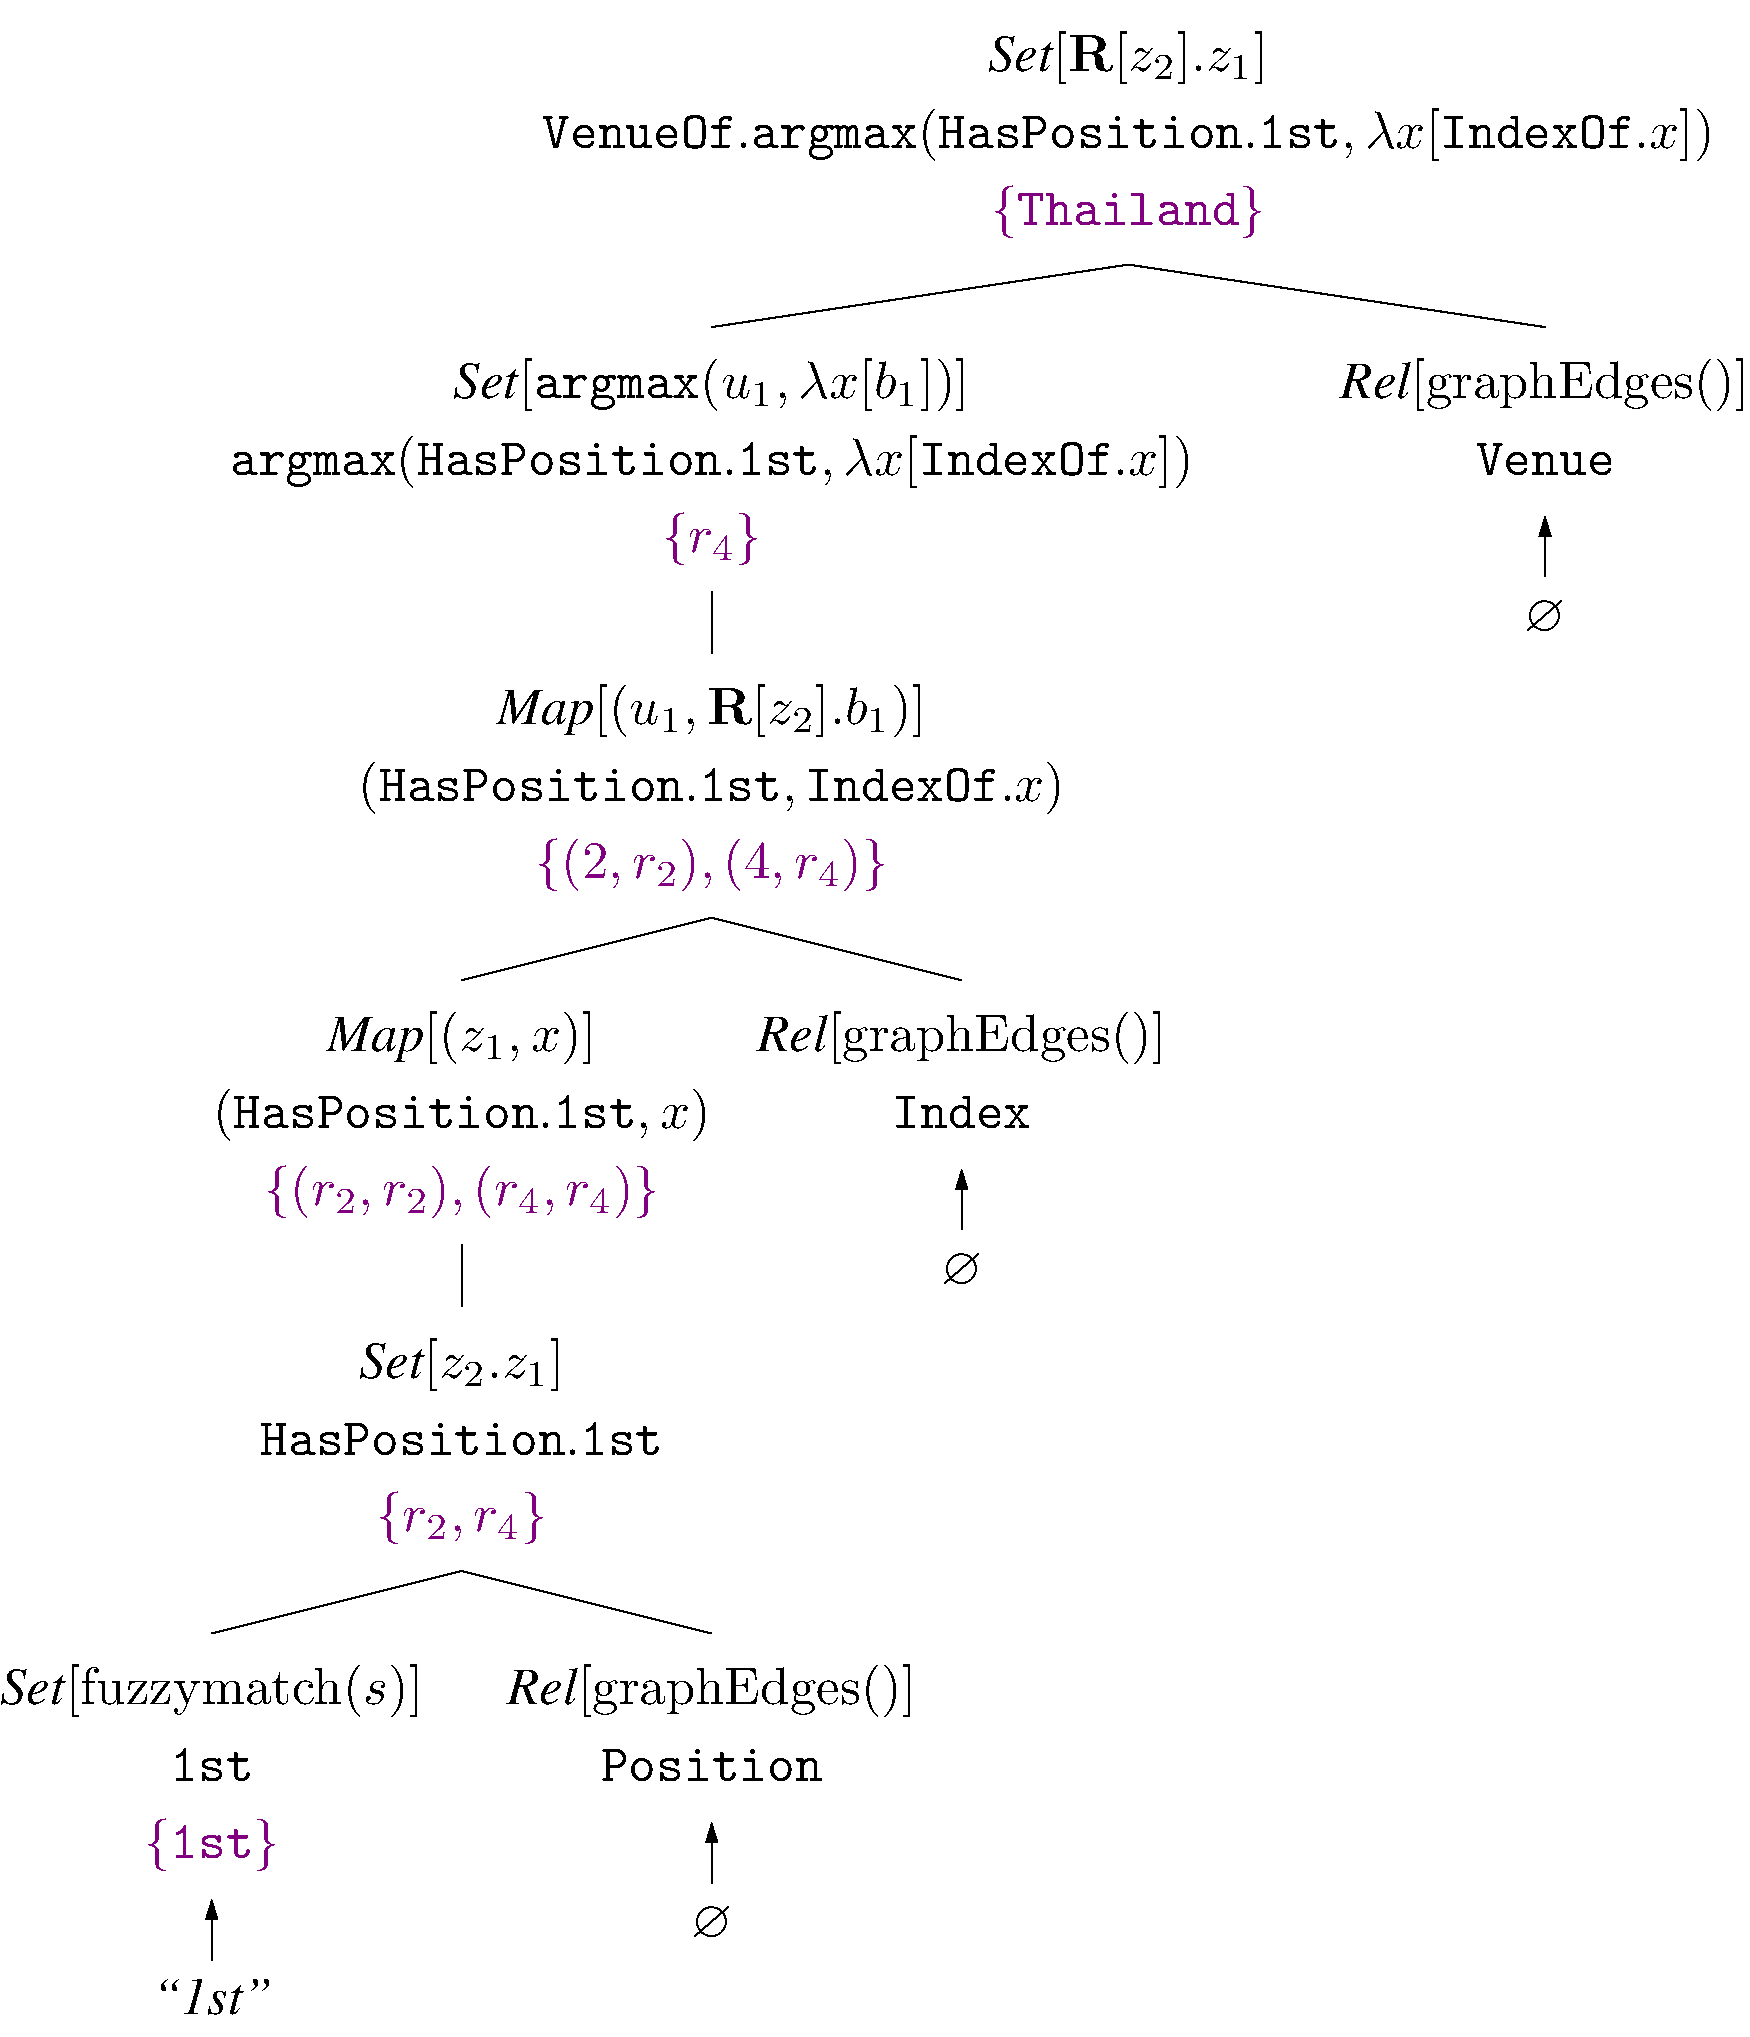
\includegraphics[scale=0.35]{sfig/parsetrees.slides/dpdParse.pdf}
\caption[Derivation tree of the running example under the \C{Map} construct.]
{A derivation tree for the utterance \runningEx
under our new set of deduction rules.
The denotations are shown in {\color[rgb]{.5, 0, .5}purple}.}
\label{fig:dpd-parse-ex}
\end{figure}

On top of the additional deduction rules,
we also introduce two new normalization edges to
the knowledge graph.
First, we use
\T{Num2} for the second number in the cell,
which usually denotes
a score of the opposing team or a measurement
in an alternative unit
(e.g., the cell node with text \nl{3--4} has
a \T{Num2} edge to atomic value \C{4}).
Second, we use
\T{Part} for items in a list
under a set of predefined list delimiters
(e.g., the cell with text
\nl{PC, Mac, Linux} has three \T{Part} edges
to \T{PC}, \T{Mac}, and \T{Linux}).
The $\Mr{fuzzymatch}$ method in Rule~T1
can generate these nodes representing cell parts
based on the utterance token spans.

\subsection{Dynamic programming on denotations}

From the deduction rules,
we could use our floating parser beam search to generate a set
of logical forms.
However, due to the generality of our deduction rules,
the set of of possible logical forms grows quickly
as the size of the logical forms increase.
As such, partial logical forms that are essential for
constructing the desired logical forms might
fall off the beam early on, resulting in an incomplete coverage.

\paragraph{Space of denotations.}
In order to reduce the search space,
our key observation is that while the number of logical forms
explodes quickly,
the number of \emph{distinct denotations}
of those logical forms grows at a much slower pace,
as multiple logical forms can share the same denotation.
For instance, the five consistent logical forms in
Figure~\ref{fig:dpd-running}
execute to the same denotation $\set{\T{Thailand}}$,
and variations in the arguments of logical operators
would create even more logical forms with that denotation.
% We can quantify this growth by plotting the
% number of distinct logical forms and their denotations
% as the logical form size increases.
% Figure~\ref{fig:lf-growth} shows that the space of logical forms
% explode much more quickly than the space of denotations.
% \todo{Details of this experiment, or maybe push to the experiments section}

Therefore, instead of directly enumerating logical forms,
we proposed \emph{dynamic programming on denotations} (DPD).
Inspired by similar methods in programming induction
\cite{lau03programming,liang10programs,gulwani2011automating,devlin2017robustfill},
the main idea is to group logical forms
with the same denotations together.
Instead of using cells $(c, s)$ of the floating parser
(where $c$ is the category and $s$ the the logical form size),
we perform dynamic programming on cells
$(c, s, d)$ where $d$ is a denotation.
For instance, the logical form
$\xHas{Position}.\T{1st}$
belongs to the cell $(\C{Set}, 1, \set{r_0, r_2})$.

One requirement for DPD to work
is that the deduction rules
must be \emph{denotationally invariant},
meaning that the denotation of the resulting logical form
must only depend on the denotations of its child
logical forms.
For example, a compositional rule 
with semantic function $g(z_1, z_2)$
is denotationally invariant if
\begin{equation}
\deno{z_1}{w} = \deno{z'_1}{w} \;\wedge\;
\deno{z_2}{w} = \deno{z'_2}{w} \implies
\deno{g(z_1, z_2)}{w} = \deno{g(z'_1, z'_2)}{w}
\end{equation}
As a counterexample, if the execution of $g(z_1, z_2)$
involves comparing the numbers of logical operators
in $z_1$ and $z_2$,
the rule is not denotationally invariant.

All deduction rules in Table~\ref{tab:dpd-rules}
are denotationally invariant.
As such, if any of our compositional rule
with semantic function $g(z_1, z_2)$
is applied on $z_1$ from cell $(c_1, s_1, d_1)$
and $z_2$ from cell $(c_2, s_2, d_2)$,
the resulting parse will belong to the same cell
$(c, s_1 + s_2 + 1, d)$ for some denotation $d$
regardless of which $z_1$ and $z_2$ are chosen.
The same conclusion applies for
compositional rules with only one child.
We will use this fact that logical forms in the same cell
are interchangeable to compress the search space
in the DPD algorithm.

\begin{figure}
\centering
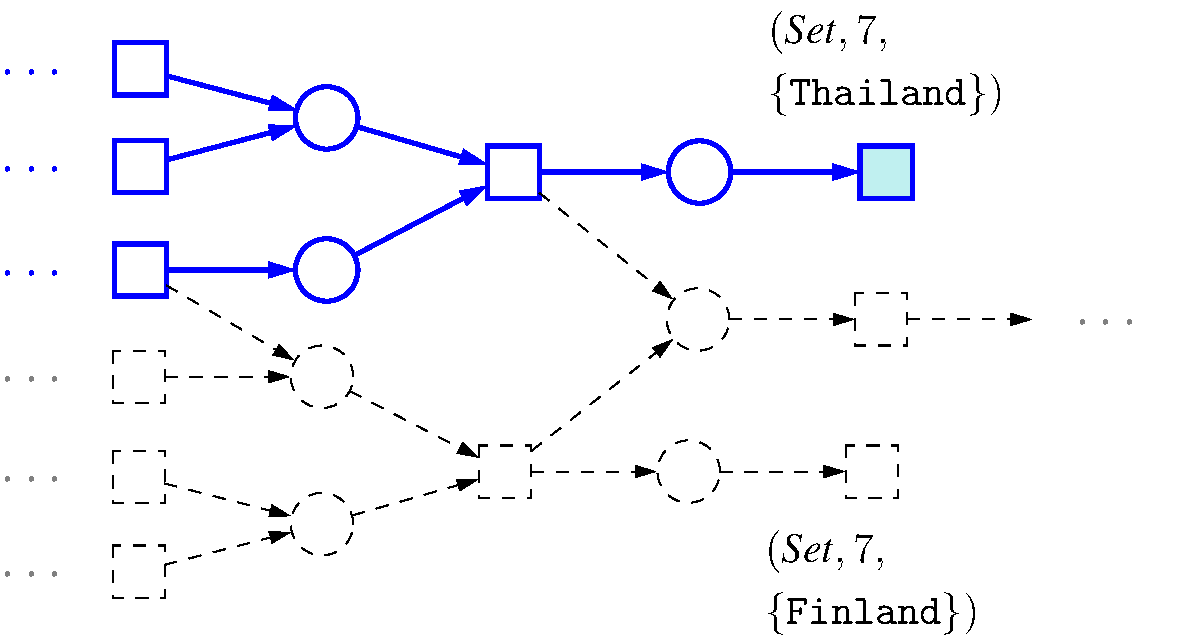
\includegraphics[scale=.4]{sfig/dpd.slides/dpdConcept.pdf}
\caption[Illustration of the DPD algorithm.]
{The first phase of DPD constructs
cells $(c,s,d)$ (square nodes)
using denotationally invariant semantic functions
(circle nodes).
The second phase enumerates all logical forms
along paths that lead to the correct
denotation $y$ ({\color{blue}solid lines}).}
\label{fig:dpd-figure}
\end{figure}

\paragraph{Algorithm.}
As illustrated in Figure~\ref{fig:dpd-figure},
the DPD algorithm consists of two phases.
The first phase finds the possible combinations of cells
$(c, s, d)$ that lead to the correct denotation $y$,
while the second phase enumerates the actual logical forms
belonging to the cells found in the first phase.

\begin{enumerate}
\item 
In the first phase,
we are only concerned about finding relevant cell combinations
and not the actual logical forms.
Therefore, any logical form that belong to a cell
could be used as an argument
of a deduction rule to construct further logical forms.
Thus, we ``collapse'' the logical forms
by keeping only at most one logical form per cell.
Subsequent logical forms generated for the same cell
are discarded,
but the combinations of children cells are recorded
for later backtracking.

After populating the cells up to some maximum size $s_\Mr{max}$,
we list all cells $(\C{Set}, s, y)$
with the correct denotation $y$,
and then note all possible cell-rule combinations
$(\Mr{cell}_1, \Mr{rule})$
or $(\Mr{cell}_1, \Mr{cell}_2, \Mr{rule})$
leading to those final cells,
including the combinations that yield discarded logical forms.

\item
The second phase retrieves the actual logical forms
by populating the cells $(c, s, d)$ with actual logical forms
using only the relevant cell-rule combinations
from the first phase.
Even though we are searching over the space of logical forms,
the elimination of irrelevant cell-rule combinations
effectively reduces the search space.
As our experiment in Section~\ref{sec:dpd-experiment} will show,
the number of cells needed to consider
is reduced by 98.7\%.
\end{enumerate}

\paragraph{Pruning.}
While denotations help us narrow down the search space,
there are a few cases where the search is still out of control.
We decide to sacrifice some generality
by introducing the following pruning procedures:

\begin{itemize}
\item We prune logical forms that are clearly redundant.
For instance, we prune any rule application that
does not change the denotation
(e.g., applying \T{max} on a set of size 1).
\item We restrict the union operation to between two cells
(e.g., $\T{Germany} \sqcup \T{Thailand}$)
since union rarely appears in other contexts.
\item We forbid the subtraction operation
when building a \C{Map}.
\item We do not allow \T{count} on a set of size 1.
This is the most restrictive heuristic since a small number
of questions require counting a set of size 1.
However, without this restriction, there are too many
logical forms that execute to $\set{1}$,
which can then be applied in other mostly irrelevant contexts
(e.g.,
selecting the first row with
$\xHas{Index}.\T{count}(z)$
where $\deno{\T{count}(z)}{w} = \set{1}$
will almost always be spurious.)
\end{itemize}

\subsection{Experiments} \label{sec:dpd-experiment}

\begin{figure}
\centering
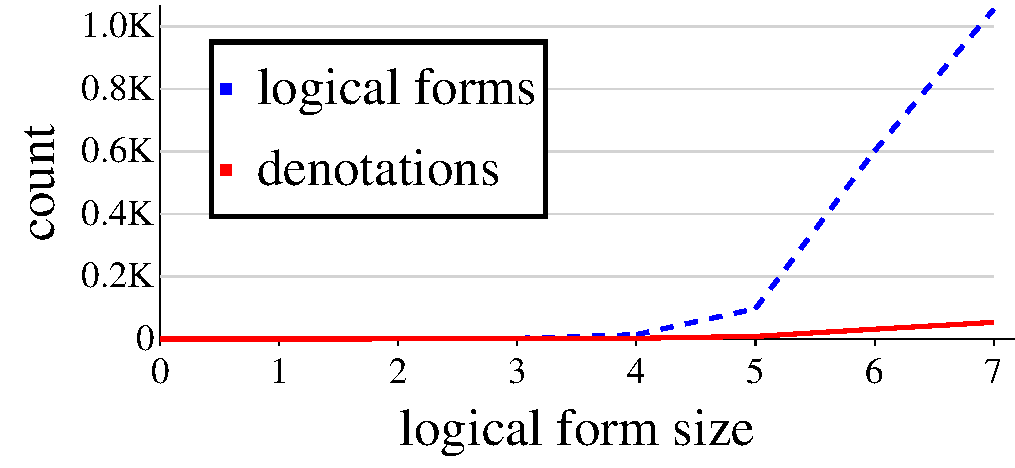
\includegraphics[scale=.4]{sfig/dpd.slides/exGrowth.pdf}
\caption[The space of denotations grows much more slowly than the space of logical forms]{The median of the number of
logical forms ({\color{blue}dashed})
and denotations ({\color{red}solid})
as the formula size increases.
The space of logical forms grows much more quickly
than the space of denotations.}
\label{fig:dpd-lf-growth}
\end{figure}

\begin{figure}[t]
\centering
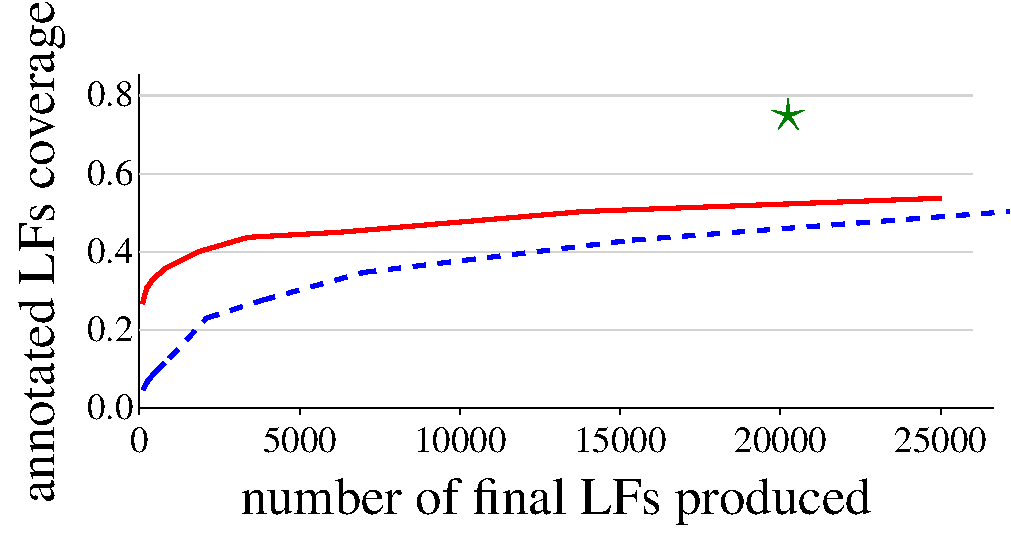
\includegraphics[scale=0.45]{sfig/dpd.slides/exFloat.pdf}
\caption[DPD has more coverage over the
annotated logical forms than beam search]{
The number of annotated logical forms
that can be generated by beam search,
both uninitialized ({\color{blue}dashed})
and initialized ({\color{red}solid}),
increases with the number of candidates generated
(controlled by the beam size),
but still lacks behind DPD ({\color{green!50!black}star}).}
\label{fig:dpd-results}
\end{figure}

% We use the training data of the \wtq dataset
% for our experiments.

\paragraph{Oracle.}
We manually annotate 300 training examples
from the \wtq dataset
with semantically logical forms if possible.
Among them, we successfully annotated 84\% of the examples,
which is a pretty good coverage since the crowd workers
who wrote the questions could have used the tables
in any way they wanted.
The remaining 16\% contains the types of reasoning
outside our setup.
Some of these include special table layouts,
answers that appear inside running texts or images
(instead of appearing as the whole cell
or a clearly demarcated part),
and questions that require common sense knowledge
(e.g., comparing \nl{Quarter-final} with \nl{Round of 16}
cannot be done by our \T{argmax}).

\paragraph{Search space.}
To demonstrate the savings gained by collapsing logical
forms with the same denotation together,
we plot the
number of distinct logical forms and their denotations
as the logical form size increases.
Figure~\ref{fig:dpd-lf-growth} shows that
the space of logical forms
explode much more quickly than the space of denotations.
Since the first phase of DPD operates
on the space of denotations,
the search is much more controlled than using beam search
over the space of logical forms.

Moreover,
DPD allows us to ignore a large number of irrelevant
partial logical forms before doing a fine-grained search
in the space of logical forms.
On average over all 14,152 training examples,
DPD generates approximately 25,000
consistent logical forms.
The first phase of DPD generates
approximately 153,000 cells $(c, s, d)$.
After filtering for the cell-rule combinations
that lead to the correct denotations,
only about 2,000 cells from 8,000 cell-rule combinations
remain, resulting in a 98.7\% reduction
of the number of cells we need to consider.

\paragraph{Coverage.}
To measure how well DPD enumerates consistent logical forms,
we consider the following experiment.
For each of the 300 training examples from earlier,
we run the DPD algorithm
to generate a set of consistent logical forms,
and then check if the annotated logical form is in the generated set.
We compare DPD against two baselines:
beam search with random parameters,
and beam search with parameters trained on the training data
of \wtq
using the method from Chapter~\ref{chp:parsing}.
The evaluation metric is coverage: the fraction of examples
where the annotated logical form is among the
generated logical forms.

Figure~\ref{fig:dpd-results}
plots the coverage against the number of logical forms
produced by the algorithms.
DPD successfully generates more annotated logical forms
(76\%)
than beam search
(53.7\%),
even when beam search is guided by the learned parameters.

\section{Filtering spurious logical forms}


\subsection{Fictitious tables}
After computing the set $\zcx$ of consistent logical forms,
the next step is to filter out spurious logical forms.
Unfortunately,
spurious logical forms and semantically correct ones
cannot be distinguished solely by considering their denotations
with respect to the table,
since the denotations will be identical by definition.
Instead, we use the following key observation:
if the same answer is asked on a different but similar tables
(e.g., having the same table schema but different cell contents),
semantically correct logical forms should give
a correct answer to the question in the new contexts,
while spurious logical forms will inevitably
fail in some contexts.
This is similar to how test cases are used to test programs:
a semantically correct program should correctly handle
the test inputs that follow the program's input specification,
while buggy programs may fail some test cases.

\begin{figure}[t]
\centering
\textsf{
\begin{tabular}{|c|c|c|c|c|} \hline
\textbf{Year} & \textbf{Venue} & \textbf{Position} & \textbf{Event} & \textbf{Time} \\ \hline
2001 & Hungary & 2nd & 400m & 47.12 \\
2003 & Finland & 1st & 400m & 46.69 \\
2005 & Germany & 11th & 400m & 46.62 \\
2007 & Thailand & 1st & relay & 182.05 \\
2008 & China & 7th & relay & 180.32 \\ \hline
\end{tabular}
}\\[.5em]$\downarrow$\\[.5em]
\textsf{
\begin{tabular}{|c|c|c|c|c|} \hline
\textbf{Year} & \textbf{Venue} & \textbf{Position} & \textbf{Event} & \textbf{Time} \\ \hline
2001 & Finland & 7th & relay & 46.62 \\
2003 & Germany & 1st & 400m & 180.32 \\
2005 & China & 1st & relay & 47.12 \\
2007 & Hungary & 7th & relay & 182.05 \\ \hline
\end{tabular}
}
\caption[
An example fictitious table.
]{
An example fictitious table generated from the table
in our running example.
}
\label{fig:fictitious-table}
\end{figure}

\paragraph{Generating fictitious tables.}
Based on the observation above,
we generate \emph{fictitious tables}
$w_1, w_2, \dots$ where each table $w_i$ is a slight
alteration of the original table $w$.
As illustrated in Figure~\ref{fig:fictitious-table},
the fictitious tables
maintain the original table schema (i.e., columns names),
but the cells in each column are re-sampled
from the pool of cell contents collected from
the original column.
The sampling process follows several guidelines:

\begin{itemize}
\item
If the cell contents of that column are originally all distinct,
sampling is done without replacement (i.e., the cells are permuted).
Otherwise, sampling is done with replacement.
\item
We want the cell predicates in the logical forms $z \in \zcx$
to be present in the fictitious table $w_i$.
To do so, any cell predicates that can be
generated by the terminal rules in Table~\ref{tab:dpd-rules}
need to appear in $w_i$.
\item
Columns where the cells are sorted usually have special semantics.
For instance, in Figure~\ref{fig:fictitious-table},
the latest event can be identified by performing \T{argmax}
on either the dates (literal semantics)
or the row indices (implied semantics: the rows are ordered
chronologically).
While one could argue that performing \T{argmax} on row indices
is spurious
under other contexts,
we will make a judgment call and decide that both approaches
are both semantically correct.
%\todo{Justify?}
As such, when constructing a fictitious table $w_i$,
we choose to keep sorted columns sorted
to preserves the implied semantics.
\end{itemize}

\begin{figure}[t]
\centering
\begin{tabular}{c|c|c|c|c@{}c@{ }l}
\multicolumn{1}{c}{} & \multicolumn{1}{c}{$w$} &
\multicolumn{1}{c}{$w_1$} & \multicolumn{1}{c}{$w_2$} & $\cdots$ \\ \cline{2-4}
$z_1$ & Thailand & China & Finland & $\cdots$ & \multirow{3}{*}{\Bigg\}} & \multirow{3}{*}{$q_1$} \\
$z_2$ & Thailand & China & Finland & $\cdots$ & \\ 
$z_3$ & Thailand & China & Finland & $\cdots$ & \\
$z_4$ & Thailand & Germany & China & $\cdots$ & \multirow{1}{*}{\}} & \multirow{1}{*}{$q_2$} \\
$z_5$ & Thailand & China & China & $\cdots$ & \multirow{2}{*}{\Big\}} & \multirow{2}{*}{$q_3$} \\
$z_6$ & Thailand & China & China & $\cdots$ & \\
$\vdots$ & $\vdots$ & $\vdots$ & $\vdots$ & \\ \cline{2-4}
\end{tabular}
\caption[Logical forms with the same denotation tuples are grouped into the same equivalence class]{
Consistent logical forms $z_i \in \zcx$
are executed on fictitious tables to get denotation tuples
$\deno{z_i}{W}$.
Logical forms with the same denotation tuple
are grouped into the same equivalence class $q_j$.}
\label{fig:equivalence-classes}
\end{figure}

\paragraph{Equivalence classes.}
Fictitious tables can help us identify logical forms
that are semantically equivalent
(under our assumption of implied column semantics above).
Let $W = (w_1, \dots, w_k)$ be a tuple of all possible
fictitious tables.
For a logical form $\zcx$, we define
its \emph{denotation tuple} as
$\deno{z}{W} = (\deno{z}{w_1}, \dots, \deno{z}{w_k})$.
We can now create equivalence classes $q$
of logical forms with the same denotation tuple,
which we will denote by $\deno{q}{W}$. 
For instance, in Figure~\ref{fig:equivalence-classes},
the logical forms $z_1$, $z_2$, and $z_3$ have the same
denotation across all fictitious tables,
and thus we group them into an equivalence class $q_1$.

When the question is unambiguous,
we expect at most one equivalence class
to contain semantically correct logical forms.

\subsection{Annotation}
To filter equivalence classes with spurious logical forms,
we acquire the correct answer to the question $x$
with respect to each fictitious table $w_i$ in $W$
from humans (e.g., via crowdsourcing).
We can filter out equivalence classes
whose denotation tuple does not match the annotated answers,
and then compile the rest into the collection $\zsx$
of semantically correct logical forms.

However, it is impractical and usually redundant
to collect the answer for all exponentially many fictitious tables.
So instead, we will approximate the process
by selecting some subset
$W' = (w'_1, \dots, w'_\ell)$ of $\ell$ fictitious tables
to be annotated with answers.

\paragraph{Choosing tables to annotate.}
We want to choose a subset $W'$ that can potentially
give us the most information about the correct equivalence class
as possible.
Let $\Mc{Q}$ be the collection of all equivalence classes.
Using the denotation tuples with respect to
$W' = (w'_1, \dots, w'_\ell)$,
we can divide $\Mc{Q}$ into partitions
\begin{equation}
F_t = \set{q \in \Mc{Q} : \deno{q}{W'} = t},
\end{equation}
where $t$ is a denotation tuple of length $\ell$.
For instance, in Figure~\ref{fig:equivalence-classes},
if $W'$ contains only $w_2$, then $q_2$ and $q_3$
will belong to the same partition $F_{(\T{China})}$.

Let the human-annotated answers form a tuple
$t^* = (y'_1, y'_2, \dots, y'_k)$.
Assuming that there is
at least one semantically correct logical form,
and that the human annotations are correct,
the answer tuple $t^*$ will identify exactly
one partition $F_{t^*}$.
This partition will include the
semantically correct equivalence class,
but can also include spurious equivalence classes
that are indistinguishable from the correct one based
on the fictitious tables in $W'$.
Our goal is to make the partitions as
\emph{small and numerous} as possible,
so that no matter what answer $t^*$ we get from humans,
the matched partition $F_{t^*}$ is likely to be small
(i.e., a large number of spurious logical forms are pruned away).

To make our objective more formal,
we choose $W'$ that maximizes
the \emph{expected information gained}
%(or equivalently, the reduction in entropy)
about the correct equivalence class given the annotation.
Define a random variable $Q \in \Mc{Q}$
representing the correct equivalence class,
and another random variable $T^*(W')$
for the annotation tuple
(which depends on our choice of $W'$).
Our objective is to find
\begin{equation}
W'
= \argmax_{W'} \nail{\HH[Q] - \HH[Q \mid T^*(W')]}
= \argmin_{W'}\;\HH[Q \mid T^*(W')],
\end{equation}
where the entropy terms $\HH[\cdot]$
measure the expected information,
and we want the entropy to reduce as much as possible
after observing the annotation.

We assume a uniform prior on the correct equivalence class $Q$:
\begin{equation}
p(Q = q) = \frac{1}{\card{\Mc{Q}}},
\end{equation}
and assume that the annotation is accurate with respect to $Q$:
\begin{equation}
p(T^*(W') = t \mid Q = q) = \cases{
1 &\cif{\deno{q}{W'} = t} \\
0 &\cotherw.}
\end{equation}
We can write
\begin{align}
p(T^*(W') = t, Q = q) &= \cases{
1/\card{\Mc{Q}} &\cif{\deno{q}{W'} = t} \\
0 &\cotherw} \\
p(T^*(W') = t) &= \frac{\card{F_t}}{\card{\Mc{Q}}}
\end{align}
(there are $\card{F_t}$ equivalence classes with
$\deno{q}{W'} = t$ due to the definition of $F_t$),
and therefore
\begin{align}
\HH[Q \mid T^*(W')]
&= -\sum_{q,t}p(q,t)\log \frac{p(q,t)}{p(t)} \\
&= -\sum_t \sum_{q; \deno{q}{W'} = t}
\frac{1}{\card{Q}}
\log \frac{1/\card{Q}}{\card{F_t}/\card{\Mc{Q}}} \\
&= \frac{1}{\card{\Mc{Q}}} \sum_t \card{F_t}\log \card{F_t}.
\label{eq:f-log-f}
\end{align}
We can search for $W'$ that minimizes
the term~(\ref{eq:f-log-f}) above.
This matches our original intuition
as the term is small
when the partitions $F_t$ are small and numerous.

In practice, we make a few more approximations:
\begin{itemize}
\item The full tuple $W$ of fictitious tables
is approximated as $k = 30$ randomly generated tables.
We then choose $W'$
by exhaustively searching over all possible combinations
of $\ell = 5$ fictitious tables.
\item We cannot guarantee that the annotations are all correct.
In our experiments, we propose several methods to trade off
accuracy with the amount of pruned spurious logical forms.
\end{itemize}

\subsection{Experiments}
We continue our investigation on the training examples
of the \wtq dataset.
The set $\zcx$ of consistent logical forms are computed
by the DPD algorithm.

\paragraph{Equivalence classes.}
Using 30 randomly generated fictitious tables,
we get an average of 1,237 equivalence classes per example.
To measure how well the true equivalence classes
(based on all possible fictitious tables)
are approximated by using on 30 fictitious tables,
we verify the equivalence classes against the ones
computed on 300 fictitious tables.
We found that only 5\% of the logical forms are separated
from the original equivalence classes.

\paragraph{Oracle annotation.}
For each of the 252 examples that were annotated
with semantically correct logical forms $z^*$
in Section~\ref{sec:dpd-experiment},
we use the denotation tuple $t^* = \deno{z^*}{W'}$
to simulate perfect human annotations.

By choosing a subset $W'$ of 5 fictitious tables that minimizes
our proposed objective function~(\ref{eq:f-log-f}),
we are able to prune out 98.7\%
of the spurious equivalence classes,
which equate to 98.3\% of spurious logical forms.
Additionally,
we were able to filter down to just one
equivalence class in 32.7\% of the examples,
and down to three classes in 51.3\% of the examples.
When more than one equivalence classes remain,
most of the time only one class will contain many
equivalent logical forms,
while other classes are small and contain
unusual logical forms such as the spurious $z_5$
in Figure~\ref{fig:dpd-running}.

If the 5 fictitious tables in $W'$ are chosen at random
instead of using our proposed method,
the number of examples that can be filtered down to
one and three classes reduce from 32.7\% to 22.6\% and
from 51.3\% to 36.5\%, respectively.

The average size of the equivalence class
containing the annotated logical form
is approximately 3,000
with a standard deviation of approximately 8,000.
As our logical formulation is very expressive,
there are many different logical forms
that equivalently represent the same semantics.

\paragraph{Human annotation.}
We now consider the answer tuple $t^*$
collected from crowdsourcing on Amazon Mechanical Turk.
We use 177 examples where at least two crowd workers
agree on the answer of the original table $w$.

The crowdsourced data is more susceptible to errors.
When using the answers on all 5 fictitious tables
to filter equivalence classes,
the entire set $\zcx$ of consistent logical forms
are pruned away in 11.3\% of the examples,
and the semantically correct equivalence class is pruned
in 9\% of the examples.
These errors are caused by annotation errors,
inconsistent data in the tables
(e.g., the \emph{Total} column
for sport medals
does not match the sum of the
\emph{Gold}, \emph{Silver}, and \emph{Bronze}
columns),
and different interpretation of the questions
on the fictitious tables.
For the remaining example,
we are able to filter out 92.1\% 
of spurious logical forms (which equates to
92.6\% of spurious equivalence classes).

To prevent semantically correct logical forms
from being pruned,
we relax our assumptions and keep any equivalence class
that disagree with the annotation $t^*$
in at most one fictitious tables.
The number of times the entire $\zcx$
is pruned out is reduced from
11.3\% to to 3\%,
but the number of spurious logical forms pruned
also decreases from 92.1\% to to 78\%.

\section{Using the generated logical forms}
The generated st $\zsx$ of semantically correct logical forms
can be used to train semantic parsers
that take logical forms as supervision.
For instance, \cite{krishnamurthy2017neural}
trains a neural semantic parser
by maximizing the log-probability of generating
100 shortest logical forms from $\zsx$.
By using the list $\zsx$,
the model does not need to perform search
during training.
Their single model achieves a test accuracy of 43.3\%,
while the ensemble model achieves an accuracy of 45.9\% .

Filtering spurious logical forms with fictitious tables
also turns out to be crucial.
When the model in \citet{krishnamurthy2017neural}
is trained on the set $\zcx$ of consistent logical forms
generated by DPD instead of the filtered $\zsx$,
the accuracy of the single model drops from 43.3\% to 36.3\%
\cite{mudrakarta2018it}.

\section{Related work and discussion}

\paragraph{Types of supervision for semantic parsing.}
As stated in the related work chapter 
(Section~\ref{sec:rw-knowledge-based-qa}),
machine learning models for semantic parsers
were mainly trained with logical forms as supervision
\cite{tang01ilp,wong07synchronous,zettlemoyer07relaxed,jia2016recombination,dong2016logical,zhong2017seq2sql}.
The logical forms provide a clear and semantically correct
signal, but they are expensive to annotate,
and the logical formalism would prematurely restricts the types
of questions present in the dataset.
Furthermore, as \citet{kushman2013regex} argues,
the annotated logical forms might not be the one
that best align with the utterance among
the equivalent logical forms.

Learning a semantic parser from denotations
\cite{clarke10world,liang11thesis,berant2013freebase}
was mainly motivated by the easiness of acquiring
annotated data.
However, for a broader domains and complex questions,
searching for semantically correct logical forms
become more difficult.
Some work tries to sidestep search,
such as by representing the process for computing answers
as continuous vectors instead of discrete symbols \cite{yin2016neural,neelakantan2016neural}.
% Others inject prior domain knowledge
% to bias the model toward semantically correct interpretations
% \citex.
Our work provides a general solution by converting
the distant supervision into direct supervision,
which opens the door for the large class of models that use
logical forms as supervision.

Previous works also considered other types
of supervision.
Without annotated logical forms or denotations,
GUSP \cite{poon2013gusp}
learns to translate dependency parses into semantic parse
by encouraging the result to be consistent with
the database schema.
\citet{krishnamurthy2012weakly} and
\citet{reddy2014large} encourage agreement
between the semantic parse and some other structure
(syntactic parse or semantic graph)
derived from the same declarative sentence.
Several previous works use interactive data,
such as dialog sessions or user feedback,
as a weak signal for interpreting the previous utterance
\cite{artzi11conversations,iyer2017neural,labutov2018learning}.

\paragraph{Test-driven program synthesis.}
The process of finding logical forms consistent
with the denotation is closely related
to test-driven program synthesis in the
programming language community.
The goal of program synthesis is to generate a program
that satisfies some specification,
such an input-output pairs.
Previous work has devised a similar idea
of dynamic programming on denotations
on more restricted spaces of programs
\cite{lau03traces,liang10programs,feser2015synthesizing,yaghmazadeh2016hierarchy},
When the program predicates are invertible,
such as in string manipulation
\cite{gulwani2011automating, parisotto2017sql, devlin2017robustfill},
the search can be made even more efficient.
More recently, \citet{wang2017program}
applies a similar technique to DPD on program synthesis,
but goes a step further to collapse
denotations of the same classes together
as another layer of abstraction.
However, doing so requires a bit more machinery
during unpacking to search over
logical forms.

\paragraph{Limitations of DPD.}
Dynamic programming on denotations depends on two assumptions
about the search space.
First, the number of unique denotations must be low
to prevent the number of cells in Phase 1 from exploding.
This means some logical form patterns, such as
arbitrary unions or subtraction between \C{Set}s or \C{Map}s,
cannot be handled effectively.
Luckily, such patterns do not occur often in the distribution
of natural questions.
Second, the number of unique logical forms that execute
to each denotation must be low; otherwise,
Phase 2 will have to search over too many logical form combinations.
One particular consequence is that \T{count} logical forms with
denotation $\{1\}$ will make the search space explode,
since many generated logical forms execute to sets of size 1.
This unfortunately reduces the coverage over correct logical forms
by approximately 2\%.

\paragraph{Test case generation.}
Our fictitious tables
functions similarly to test cases.
Previous work has considered generating
new test cases \cite{miller1990empirical},
but the goal there is to converge on a single program
rather than identifying a class of programs.

\paragraph{Avoiding spurious logical forms.}
When training with distant supervision,
the model can incorrectly updates toward spurious logical forms
found during search.
One way to avoid this without using additional annotations
is to ``hedge'' the updates:
in early training iterations,
perform updates toward consistent logical forms more equally
instead of proportionally to the probabilities assigned by the model.
This intuition, coupled with decoding strategies
that encourage more exploration,
can prevent the model from making bad updates toward spurious logical forms
\cite{guu2017bridging,misra2018policy}.

\section{Conclusion}
In this chapter,
we presented techniques for converting
distant supervision (denotations) into direct supervision
(logical forms).
Given the correct answer for a question
we efficiently enumerate logical forms consistent with the answer
using dynamic programming on denotations,
and then filter out spurious logical forms
with fictitious tables.
The resulting set of logical forms
can be used to train a directly supervised parser,
effectively sidestepping search problems during training.

The value of having logical forms as direct supervision
has been noted by \citet{yih2016value},
who used a labeling interface to annotate
questions in the \Sc{WebQuestions} dataset \cite{berant2013freebase}
with SPARQL queries.
Training with annotated queries as supervision
yields an increased accuracy,
and compared to the distantly supervised model,
the number of incorrect relations
%many errors that the model trained on denotations make
%are due to incorrect relations
learned through spurious logical forms
is decreased.
Our method of pre-computing logical forms
provides a more automatic method for annotating
examples with logical forms than the annotation interface.
While it still requires some human effort,
we do not require experts even when annotating complex questions.

Up to this chapter,
we have considered a new QA task that operates
on a high-\Breadth high-\Depth regime,
as well as algorithms based on semantic parsing 
to tackle the task.
The next chapter concludes our findings,
lists alternative QA methods in the literature
for solving our proposed task,
and provides several potential paths for future work.


\chapter{Conclusion}
\label{chp:conclusion}
\section{Summary}

\paragraph{New QA tasks with increased \Breadth and \Depth.}
In this dissertation, we focus on improving the capability
of question answering systems
%natural language interfaces, such as virtual assistants
%and natural language interface to databases,
along two axes.
First, to increase the scope of the knowledge sources
that the systems operate on
(\Breadth), we consider using web pages,
which contain open-domain semi-structured data,
as the knowledge source
(Chapter~\ref{chp:semi}).
As tabular data on web pages contain computable knowledge
suitable for complex reasoning,
we propose the task of answering compositional questions
on web tables,
which aims to increase task complexity (\Depth)
and the scope of the knowledge source simultaneously
(Chapter~\ref{chp:tables}).
For the task,
we have collected a new \wtq dataset of complex questions
on tables and their answers.
The dataset contains comparable or higher task complexity,
as well as a broader open-domain knowledge source,
than contemporary semantic parsing datasets.

\paragraph{Training a semantic parser from denotations.}
We cast the proposed QA task as learning
a semantic parser using the annotated answers as
distant supervision (Chapter~\ref{chp:parsing}).
We address the increased question complexity (\Depth)
by using compositional logical forms
to express the multiple steps needed for computing answers.
To construct candidate logical forms,
the parser uses a set of deduction rules
to build larger logical forms from smaller parts.

Meanwhile, to address the potentially unseen
table schema (\Breadth),
we represent tables with
schema-independent knowledge graphs,
and then use floating deduction rules to flexibly generate
open-domain logical form predicates
based on the table.
In contrast to offline information extraction,
which assumes a fixed and canonicalized database schema,
our on-the-fly information extraction approach
can adapt to arbitrary data schemata and
maintain uncertainty over the possible interpretations
of the table.
This ultimately allows us to answer a wider range
of open-domain questions.

\paragraph{Speeding up the parser.}
The coverage over answerable questions can be increased
by expanding the set of deduction rules
and augmenting the knowledge graph representation.
To compensate for the increased space of logical forms
from this expansion,
we proposed a way to improve search
by reusing useful logical form patterns
(Chapter~\ref{chp:macro}).
When processing an input question,
similar questions in the training dataset are retrieved,
and the logical form macros from those questions
are used to construct logical forms.
This allows the parser to skip the generation of
logical forms that are less likely to be a good parse.

\paragraph{Converting distant supervision to direct supervision.}
Training a parser with distant supervision requires
performing search during training,
which introduces several challenges.
With the expanding space of logical forms,
it is more difficult to find logical forms consistent
with the correct answer during training,
and the discovered logical forms might be spurious
(right for wrong reasons),
leading to bad parameter updates.
We propose to factor out the search
and precompute the semantically correct logical forms
for each example,
which effectively converts the dataset into
a directly supervised one (Chapter~\ref{chp:dpd}).
The resulting logical forms
can then be used to train a parser
that takes logical forms as supervision
without having to perform search during training.

\section{State-of-the-art on the \wtq dataset}

\begin{table}[t]
\centering
\begin{tabular}{lrr} \toprule
& \multicolumn{2}{c}{\textbf{Test accuracy}} \\
\cmidrule{2-3}
\textbf{System}
& \textbf{Single model}
& \textbf{Ensemble} \\ \midrule
Original deduction rules (Chapter~\ref{chp:parsing})
& 37.1
& - \\
Expanded deduction rules (Chapter~\ref{chp:macro})
& 42.7
& - \\
Expanded deduction rules + macros (Chapter~\ref{chp:macro})
& 43.7
& - \\ 
\midrule

Neural Programmer \cite{neelakantan2017learning}
& 34.2
& 37.7 \\
Neural Multi-Step Reasoning \cite{haug2018neural}
& 34.8
& 38.7 \\
Rule-based + Abductive Matching \cite{dhamdhere2017abductive}
& 40.4
& - \\
Neural Decoding with Type Constraints \cite{krishnamurthy2017neural}
& 43.3
& 45.9 \\
Memory Augmented Policy Optimization (MAPO) \cite{liang2018mapo}
& 43.9
& 46.3 \\
MAPO + Meta Reward Learning \cite{agarwal2019learning}
& 44.1
& 46.9 \\
MAPO + Neural Program Planner \cite{biloki2019neural}
& 43.9
& 47.2 \\
\bottomrule

\end{tabular}

\caption{Test accuracy of the previous work
on the \wtq dataset.}
\label{tab:conclude-sota}
\end{table}

Table~\ref{tab:conclude-sota}
summarizes previous work on the \wtq dataset.
Descriptions and insights of the methods and their related works
are described below.
The annotated answers are used as distant supervision
unless stated otherwise.

\subsection{Using continuous representations for computation}

Logical form operators are interpretable
and efficient to execute.
However,
a system generating such symbolic operators as discrete actions
cannot be trained end-to-end with backpropagation.
As an alternative,
the following works consider using 
differentiable operators
to represent the steps of computing the answer.

\begin{itemize}
\item 
Neural Programmer \cite{neelakantan2016neural,neelakantan2017learning}
proposes to model the operators as predefined continuous functions
such as matrix multiplication and pooling.
At each time step, the model
applies each operator on the current state vectors,
and then compute a weighted average of the results
(where the weight of each operator is predicted by the model)
to be used as new state vectors.
The final state vectors are used to compute the final answer.

Since all operators are differentiable,
the model can be trained end-to-end with backpropagation
from distant supervision.
The model will have to learn to compute the weights of the operators
based on the input utterance and table.

\item
Similar to Neural Programmer,
Neural Enquirer \cite{yin2016neural}
also uses continuous functions to model the steps of computation.
However,
the hand-engineered networks for the operators in Neural Programmer
are replaced with a single general network
for computing the state vectors.
The network can be trained using a loss function
defined on the final denotation.
The system is evaluated on synthetic questions that are compositional
but closed-domain.

\item
The work by \citet{mou2017coupling}
models the steps of computations in two ways:
continuous functions,
which are trained end-to-end;
and symbolic operators,
whose decoder is trained with REINFORCE \cite{williams1992simple}.
The key observation is that parts of the state vectors
from the continuous functions are interpretable
(e.g., as attention over table rows).
Such information
can serve as a guidance when learning to decode symbolic operators.
This helps mitigate the cold start problem
of REINFORCE by boosting the chance of getting reward
when training the symbolic decoder.
The system is evaluated on the dataset by \citet{yin2016neural} above.

\end{itemize}

Continuous operators allows the model to be trained
in an end-to-end fashion from denotations without having to
perform search.
However, it can be difficult to design or learn new operators
to perform more complex reasoning;
for instance, adding an operator to subtract one column from another
would require either a careful design for a predefined operator,
or a large amount of training data for a trainable operator.
Trainable operators like in \citet{yin2016neural}
and \citet{mou2017coupling} are also less interpretable
than the discrete logical forms.

\subsection{Different generation and scoring mechanisms}

The following works use logical forms to represent
the steps of computation,
but employ different methods for generating
and scoring the logical forms.

\begin{itemize}

\item Neural Multi-Step Reasoning \cite{haug2018neural}
uses the floating parser (Chapter~\ref{chp:parsing})
to generate logical form candidates,
but then applies a neural scorer to score logical forms.
In particular, the scorer uses
pre-trained word embeddings and information from the table to
embed the utterance
and a natural language paraphrase of the logical form
into the same space.
The similarity score between the two embeddings becomes the score
of the logical form.

\item The work by \citet{dhamdhere2017analyza,dhamdhere2017abductive}
uses a rule-based system to
process the table,
generate semantic parses from the input,
and score them.
To fill in the operands that the rule-based system cannot handle well
(e.g., matching the phrase \nl{movie} to the column \emph{Title}),
a machine learning system is trained to perform abductive reasoning
and infer the missing values.
The rule-based system is easy to debug
and generates a controllable number of parses
(8.7 on average as opposed to exponentially many parses from the
floating parser),
while the machine learning part helps with
the difficult and open-domain predicates.

\item Neural Decoding with Type Constraints \cite{krishnamurthy2017neural}
trains a top-down symbolic decoder using the logical forms
generated by DPD and fictitious tables (Chapter~\ref{chp:dpd})
as supervision.
Type constraints mined from logical forms
are used to ensure the validity of the output,
as well as to control the space of possible actions at each time step.

\item Memory Augmented Policy Optimization (MAPO) \cite{liang2018mapo}
applies a policy gradient algorithm to train an agent
that generates logical forms in Lisp-like syntax.
To address the cold start problem when training from a random policy,
the work introduces (1)
systematic exploration that caches the explored trajectories
so that consistent logical forms are found more quickly;
(2) a memory buffer
for storing logical forms with high reward;
and (3) an unbiased low-variance policy gradient update
that incorporates both logical forms in the memory buffer
and on-policy trajectories.
Later works improves the reinforcement learning part
with meta reward learning \cite{agarwal2019learning}
and a model-based program planner \cite{biloki2019neural}.

% \item The Sequential Question Answering dataset \cite{iyyer2017search} \todo{}

% \item \citet{misra2018policy} \todo{}

\end{itemize}

\section{Future directions}

\paragraph{Knowing when to abstain.}
Our main evaluation metric, accuracy,
encourages the model to always predict an answer
even when (1) the question cannot be answered from the given context,
and (2) the model is not confident about the answer.
This is problematic is real-world settings
where precision is more important than recall;
for instance, a virtual assistant should not perform actions
with misleading or disastrous consequences
\cite{dhamdhere2017abductive}.
One possible future direction is to make a model
that can abstain from answering a question,
and can make a trade-off between precision and recall
\cite{yao2014freebase,rajpurkar2018squadrun,dong2018confidence}.

\paragraph{Avoiding the long tail of phenomena.}
\wtq is a challenging dataset containing both compositional utterances
with little constraints, and tables with arbitrary data and formatting.
As such, while the model errors can be categorized at a high-level
(Section~\ref{sec:sempre-error-analysis}),
addressing an individual error type with some heavy machinery
would push up the score by only a small amount.
Moreover, interesting phenomena
that occur less frequently in the dataset
will likely to be ignored by the model.

One alternative solution is to come up with a family of datasets,
each focusing on some particular challenge (e.g., rare logical operators
or table understanding) while keeping the rest fixed.
This way, methods for handling the phenomena could be developed
more quickly with clear results.
Another potential solution is to gather new examples
for the rare phenomena in an interactive fashion.

\paragraph{Combining information from multiple sources.}
Finally, the tasks introduced in this dissertation
are limited to using one source of data for all computation steps.
In reality, the information needed to perform a task
is often scattered around in multiple knowledge sources.
For instance, to handle the query \nl{Direction to John's house},
the system would need to identify who John is
(e.g., by finding a close friend on Facebook with name John),
find his address
(e.g., by looking up on John's personal web page),
and then find the direction
(e.g., using GPS and a map application).

Several question answering and semantic parsing datasets
such as QALD \cite{lopez2013evaluating},
Spider \cite{yu2018spider},
HotpotQA \cite{yang2018hotpotqa},
and DROP \cite{dua2019drop}
require the fusion of knowledge from multiple sources.
We believe that the ability to plan complex actions
on multiple, open-domain environments is the right path
toward an ideal natural language interface.


\appendix

\bibliographystyle{acl_natbib_nourl}
\bibliography{all}

\end{document}
